% =============================================================
% MSc Technical Activity Report — Ferrocement Corrosion Project
% Master document (minimal skeleton; front matter not yet finalised)
% =============================================================
\documentclass[11pt,a4paper]{report}

\usepackage[a4paper,margin=2.5cm]{geometry}
\usepackage[utf8]{inputenc}
\usepackage[T1]{fontenc}
\usepackage{amsmath,amssymb}
\usepackage{booktabs}
\usepackage{longtable}
\usepackage{array}
\usepackage{graphicx}
\usepackage{tikz}
\usetikzlibrary{arrows.meta,positioning,fit,backgrounds}
\usepackage{xcolor}
\usepackage[colorlinks=true,linkcolor=black,citecolor=black,urlcolor=black]{hyperref}
\usepackage{natbib}
\usepackage{caption}
\usepackage{siunitx}
\usepackage{placeins}

\graphicspath{{figures/}}

\title{Technical Activity Report\\[0.3em]
\large A Multi-Phase Investigation of Visible Corrosion and Structural
Condition in Ferrocement Specimens}
\author{Draft working document --- not for distribution}
\date{Draft in progress}

\begin{document}

% --- Front matter: title-page metadata is still a placeholder pending
% verified author/supervisor/programme details; Abstract and Executive
% Summary are finalised scientific summaries of the frozen report body.
\maketitle
\chapter*{Abstract}
\addcontentsline{toc}{chapter}{Abstract}

Corrosion of steel reinforcement is a principal durability concern for
cementitious structural elements, and repeated photography offers an
inexpensive, non-destructive way to observe it over time. This activity
uses a predecessor experimental dataset of 48 ferrocement specimens tested
across two exposure campaigns and photographed repeatedly; in the current
audited basis, 791 aligned, readable observations carry dense
visible-corrosion labels, while wire-area loss and ultimate load are each
obtained only once per specimen, at the end of its exposure period. Built
around this asymmetry between dense surface supervision and sparse
terminal structural supervision, the activity progressed through
classical, deep-embedding, and interpretable image representations of
visible corrosion; a feasibility study of hidden structural-condition
inference; robustness evaluation under grouped and transfer-based holdout
regimes; a refocused study of terminal ultimate load; and an exploratory
degradation and proxy-remaining-useful-life screening chain. Visible
surface corrosion proved the strongest and most consistently learnable
image-based quantity, although specific benchmarks carry a
label-adjacency risk and treatment-level transfer robustness proved
phase-dependent. Hidden structural inference was substantially weaker and
less transferable, and must be interpreted in light of its sparse,
terminal, campaign-confounded supervision. Image-derived features did not
provide reliable
incremental predictive value over metadata for terminal ultimate load
under pooled evaluation. Moving to treatment- and campaign-level transfer
materially changed which conclusions the evidence could support, with
campaign holdout acting as a severe extrapolation stress test given how
closely campaign identity is entangled with specimen design here. The degradation and
proxy-remaining-useful-life work is methodological and diagnostic rather
than validated prognosis: no true remaining-useful-life supervision exists
in the dataset. A leakage-safe dataset for a subsequent four-class
severity classification task was also prepared, though not yet modelled.
The activity's principal contribution is a rigorously bounded account of
what repeated corrosion imagery can and cannot support here, together with
a traceable basis for the work that should follow.

\chapter*{Executive Summary}
\addcontentsline{toc}{chapter}{Executive Summary}

\paragraph{Purpose and evidence basis.} This report documents an MSc
technical activity investigating how much can be learned about a
ferrocement specimen's condition from repeated corrosion photography. It
builds on a predecessor experimental dataset — 48 specimens fabricated,
chloride-exposed, and terminally tested across two campaigns, external to
the present activity — and works from the resulting photographic record,
specimen metadata, and terminal mechanical measurements. Visible-corrosion
labels are available for nearly every image in the current audited basis
(791 of 792 raw files), while wire-area loss and ultimate load are each
obtained only once per specimen, at the end of its exposure period. This
asymmetry between dense surface supervision and sparse terminal structural
supervision governs how every finding in this report should be read.

\paragraph{Technical activity.} The activity comprised: an audit and
alignment of the raw photographic and workbook data; three successive
approaches to visible-corrosion estimation (a classical handcrafted
baseline, a frozen deep-image embedding, and an interpretable
multi-family feature representation); a feasibility study of hidden
structural-condition inference; systematic robustness evaluation under
grouped, treatment-held-out, and campaign-held-out specimen partitions; a
refocused study explicitly testing whether images add value beyond
metadata for terminal ultimate load; an exploratory degradation-curve and
proxy-remaining-useful-life screening pipeline; preparation of a
leakage-safe dataset and augmentation pipeline for a four-class
corrosion-severity classification task; and an audit of the project's own
software and reproducibility practices.

\paragraph{Main findings.} The evidence supports a clear hierarchy of
confidence:
\begin{enumerate}
\item \textbf{Visible corrosion} is the strongest and most consistently
learnable image-based quantity in this dataset, across three distinct
representations.
\item \textbf{Hidden structural inference} is substantially weaker: the
available structural models are either mixed-input or, in their final,
most carefully selected form, metadata-only, and none transfers reliably
across campaigns.
\item \textbf{Terminal ultimate load}, one of the two directly measured
terminal structural endpoints and the endpoint selected for the
refocused analysis, is dominated by specimen and exposure metadata under
pooled evaluation; no robust incremental benefit from image-derived
features was established.
\item \textbf{Degradation and proxy-remaining-useful-life screening}
remain exploratory: the pipeline is a working demonstration of a
derivation chain, not a validated prognostic method.
\end{enumerate}
Two cross-cutting points qualify all four: which evaluation regime is used
materially changes what can be claimed, and leave-one-campaign-out is a
severe extrapolation stress test in this dataset because campaign identity
is entangled with steel-mesh configuration, chloride level, and exposure
duration. In addition, some strong visible-corrosion benchmarks rely on
image-derived features that are very closely aligned with the target,
creating shortcut or label-adjacency risk; the strongest case is the
near-reconstructive total-rust pairing identified by the later feature
audit, and this is checked and flagged explicitly where it applies.

\paragraph{Scope and limitations.} Every structural or prognostic
conclusion in this report is built on 48 terminal structural
measurements, from only two experimental campaigns whose design factors
are almost perfectly confounded with campaign identity. No specimen has a
repeated or intermediate structural measurement, and no specimen has an
observed failure or lifetime event; structural values reported at
non-terminal weeks are always model estimates, never measurements. The
four-class classification branch's data preparation is complete, but no
classifier has been trained, compared, or evaluated at the time of
writing.

\paragraph{Current status and next direction.} The main report body
(dataset audit, methodological framework, activity chronology, integrated
results, interpretation, software/reproducibility audit, limitations, and
conclusions) is complete. Reproducibility has improved over the course of
the project — deterministic augmentation, saved split manifests, and an
automated feature-diagnostics report are already in place — though two
live configuration and source-code issues, identified and located in this
report, still prevent an unmodified rerun of some pipeline stages. The
most immediately justified next modelling step is training a baseline
classifier for the prepared four-class branch, evaluated with
specimen-disjoint, class-sensitive metrics. Beyond that, materially
stronger structural or remaining-life claims will ultimately require new
experimental evidence — additional independent campaigns, decoupled
design factors, more structural-labelled specimens, repeated structural
measurements, and observed lifetime data — rather than further model
refinement alone.

\tableofcontents

% =============================================================
% Chapter 1 -- Introduction and Project Scope
% =============================================================
\chapter{Introduction and Project Scope}
\label{ch:introduction}

\section{Background and Motivation}
\label{sec:intro-background}

Corrosion of steel reinforcement is a principal durability concern for
reinforced cementitious structural elements, and ferrocement — a thin,
densely mesh-reinforced cementitious composite — is no exception. Assessing
that corrosion typically requires either destructive sampling or
specialised instrumentation, both of which are costly to apply repeatedly
over an element's service life. Repeated photography of an exposed
surface is, by contrast, comparatively inexpensive and non-destructive,
and it raises a natural question: how much can be inferred about a
specimen's condition from its accumulated photographic record alone?

Answering that question requires distinguishing two quantities that are
easy to conflate but evidentially very different. Visible surface
corrosion is directly observable in a photograph and can, in principle, be
labelled and re-labelled from the same image at any time. Internal
structural condition, by contrast, is not observed longitudinally in the
photographic record at all: structural supervision is available only
through terminal measurements — wire-area loss and ultimate load —
obtained once per specimen, destructively, at the end of its exposure
period. This report's central technical thread, developed across the
chapters that follow, is this distinction: what a dense,
repeatedly-observed surface quantity can support scientifically is not
automatically what sparse, terminal structural measurements can support,
and the two must be evaluated, and reported, differently.

The physical specimens, their fabrication, their accelerated
chloride-exposure programme, and their terminal mechanical testing are
predecessor experimental work, external to the present activity,
documented in an earlier MSc thesis \citep{hossain_thesis} and a related
conference paper \citep{artiste2025}. The present activity builds on, and
uses, the experimental dataset generated by that preceding work; it does
not repeat the physical experiment. Some of the later image-feature work
in this activity is best described as a Python reconstruction and
extension of concepts from that predecessor workflow, rather than an
exact reproduction of it (Chapter~\ref{ch:activities}). Facts about the physical experiment are
attributed to that predecessor source throughout this report; facts about
how the resulting data has been organised, audited, modelled, and
interpreted are attributed to the present activity.

\section{Project Context and Data Basis}
\label{sec:intro-context}

The dataset comprises 48 ferrocement specimens tested across two
experimental campaigns, each photographed repeatedly over its exposure
period. Visible-corrosion labels are available throughout this
photographic record — in the current audited basis, 791 aligned, readable
observations out of 792 raw image files (Chapter~\ref{ch:dataset}) — while
terminal structural measurements exist for each specimen exactly once, at
the end of its exposure period. This asymmetry between dense, repeatedly
observed visible-corrosion supervision and sparse, single-timepoint
structural supervision is the single most consequential structural fact
about this dataset, and it is why visible-corrosion estimation and
structural-condition inference are treated as scientifically distinct
problems throughout this report rather than as two readings of the same
underlying task. Chapter~\ref{ch:dataset} presents the full dataset audit;
it is not repeated here.

\section{Project Objectives and Research Questions}
\label{sec:intro-objectives}

The activity was organised around five research questions, each answered,
to varying degrees of confidence, by the work reported in
Chapters~\ref{ch:activities} and~\ref{ch:results}.

\textbf{RQ1.} To what extent can visible surface corrosion be estimated
from repeated images, using classical, deep-embedding, and interpretable
representations in turn?

\textbf{RQ2.} Can hidden structural condition, or terminal structural
response specifically, be inferred reliably from the available
image-derived and metadata inputs?

\textbf{RQ3.} Do image-derived features provide incremental predictive
value beyond known specimen and exposure metadata for terminal ultimate
load?

\textbf{RQ4.} How robust are the resulting conclusions when evaluation
moves from a grouped specimen holdout to treatment-level and campaign-level
transfer tests?

\textbf{RQ5.} What can degradation-curve fitting and threshold-based
proxy-RUL screening legitimately contribute, given the absence of repeated
structural measurements and of any observed true lifetime outcome?

A later, separate workstream — preparing a leakage-safe dataset and
augmentation pipeline for four-class visible-corrosion severity
classification — is deliberately not framed as a sixth research question
here, since it addresses data preparation rather than a modelling
question, and no classifier has yet been trained on it
(Section~\ref{sec:intro-scope}).

\section{Scope of the Technical Activity}
\label{sec:intro-scope}

The activity reported here comprises: an audit and alignment of the raw
photographic and workbook data; a classical visible-corrosion baseline; a
frozen deep-image-embedding experiment; an engineered, interpretable image
feature representation; structural-condition feasibility modelling;
robustness evaluation under grouped, leave-one-treatment-out, and
leave-one-campaign-out regimes; degradation-curve fitting and proxy-RUL
screening; a refocused study of terminal ultimate load; preparation of an
augmented, specimen-grouped dataset for four-class classification; and an
audit of the project's own software and reproducibility practices.
Chapter~\ref{ch:activities} describes each of these in turn;
Chapter~\ref{ch:engineering} covers the last.

Several boundaries on what this report claims are stated here explicitly,
because they govern how every later chapter should be read. This report
does not establish, and does not claim, a validated remaining-useful-life
model: no true RUL supervision exists in the dataset, and the
proxy-RUL construct introduced in Chapter~\ref{ch:framework} is an
explicitly qualified screening quantity, not a lifetime prediction. It
does not claim that visible surface corrosion causally determines
structural capacity; where a statistical association between the two is
reported, it is reported together with the confounding structure that
limits how it may be interpreted. It does not produce an externally
validated or deployment-ready model of any kind. It does not include a
trained four-class classifier: that branch's data preparation is complete,
but no classifier has been trained, compared, or evaluated
(Chapter~\ref{ch:activities}). And it does not treat model-estimated
structural states at non-terminal observation weeks as measurements — they
are, throughout, the output of a model, not a repeated physical
observation.

\section{Main Contributions of the Activity}
\label{sec:intro-contributions}

The activity's principal, completed contributions are as follows.

\textbf{(A)} Audited and aligned a specimen-level analysis basis from the
raw photographic and workbook data, resolving several version-specific
discrepancies across the project's successive implementation phases
(Chapter~\ref{ch:dataset}).

\textbf{(B)} Established visible-corrosion estimation as the most
consistently learnable image-based task in this dataset, while
identifying specific label-adjacency and near-tautology risks that limit
how some individual benchmarks should be read
(Chapter~\ref{ch:activities}, Chapter~\ref{ch:results}).

\textbf{(C)} Quantified the substantially weaker and less stable
transferability of hidden structural prediction, and disentangled the
contribution of image-derived inputs from metadata/campaign-linked
predictive structure through explicit ablations and transfer tests
(Chapter~\ref{ch:activities}, Chapter~\ref{ch:results},
Chapter~\ref{ch:interpretation}).

\textbf{(D)} Refocused the structural research question onto terminal
ultimate load — one of the two directly measured terminal structural
endpoints, and the one selected for this analysis — and explicitly
tested, rather than assumed, whether images add predictive value beyond
metadata for it (Chapter~\ref{ch:activities}).

\textbf{(E)} Built and critically evaluated a degradation-curve and
proxy-RUL screening chain across two independently configured
generations, establishing why its contribution is methodological and
diagnostic rather than validated prognosis
(Chapter~\ref{ch:activities}, Chapter~\ref{ch:interpretation}).

\textbf{(F)} Prepared a leakage-safe, specimen-grouped, reproducible
dataset and augmentation pipeline for a four-class visible-corrosion
severity classification task, ready for subsequent model training
(Chapter~\ref{ch:activities}).

\textbf{(G)} Documented concrete reproducibility and software-engineering
issues in the project's own codebase, and maintained a traceable,
source-cited evidence record for every quantitative claim in this report
(Chapter~\ref{ch:engineering}).

None of these is presented as a novel publication-level scientific
contribution in its own right; each is a specific, bounded piece of work
completed during this activity, reported at the level of confidence its
own evidence supports.

Read together, the activity's findings are, at a high level: visible
surface corrosion is the most consistently learnable image-based quantity
available in this dataset; hidden structural inference is substantially
weaker, and strongly affected by sparse supervision and campaign-linked
design structure; images do not show a reliable pooled incremental
benefit over metadata for terminal ultimate load under the settings
tested here; and the proxy-RUL construct remains a useful exploratory
screening tool rather than a validated prognosis of remaining service
life. The evidence and qualifications behind each of these statements are
given in full in Chapters~\ref{ch:activities}--\ref{ch:interpretation}.

\section{Report Organisation}
\label{sec:intro-organisation}

Chapter~\ref{ch:dataset} audits the dataset and establishes the
supervision asymmetry this introduction has previewed.
Chapter~\ref{ch:framework} sets out the methodological framework —
evaluation regimes, representation strategies, and the
observed/model-derived/derived-screening distinction — shared across later
chapters. Chapter~\ref{ch:activities} reconstructs the project's
successive implementation phases chronologically.
Chapter~\ref{ch:results} integrates that evidence by scientific question
rather than by phase, and Chapter~\ref{ch:interpretation} explains what
the integrated evidence means and why it justified the research decisions
taken. Chapter~\ref{ch:engineering} documents the project's software and
reproducibility practices and their current limitations,
Chapter~\ref{ch:limitations} states the limitations of the evidence itself
by category, and Chapter~\ref{ch:status} gives the current project status
and the work this report recommends next.


% =============================================================
% Chapter 2 -- Dataset, Experimental Context, and Data Audit
% =============================================================
\chapter{Dataset, Experimental Context, and Data Audit}
\label{ch:dataset}

This chapter sets out the physical experimental context, the structure of
the available data, and the outcome of a dataset-level audit that later
chapters build upon rather than re-deriving. It distinguishes between facts
about the physical experiment, which originate from predecessor work
external to the present project, and facts about how that experimental
record has been organised, cleaned, and represented within the present
project's own pipeline.

\section{Experimental Context}
\label{sec:experimental-context}

The dataset originates from a physical durability study of ferrocement
specimens subjected to accelerated chloride-induced corrosion. Ferrocement
elements reinforced with steel mesh were fabricated, exposed to a saline
environment for an extended period, and photographed repeatedly to record
the progression of visible surface corrosion. At the end of each specimen's
exposure period, a terminal mechanical test was carried out to characterise
its residual structural condition. The physical fabrication, exposure, and
testing programme was designed and executed as predecessor work, documented
in an earlier MSc thesis \citep{hossain_thesis} and a related conference
paper \citep{artiste2025}; the present project did not conduct this physical
experiment. It instead works from the photographic record, the associated
specimen/exposure metadata, and the terminal mechanical-test measurements
that resulted from it, and reconstructs a specimen-to-campaign/treatment
mapping from specimen identifiers, cross-checked against the treatment
tables reported in the predecessor thesis.\footnote{The specimen-to-campaign
and specimen-to-treatment mapping used throughout the present project's
pipeline is maintained as a single, version-controlled table that is
documented as the preferred source for this reconstruction, in preference
to the raw treatment columns present in the data workbook.}
Facts concerning the physical experiment itself are attributed to this
predecessor source; facts concerning how the present project has organised
or audited the resulting data are attributed to the present project's own
code, configuration, or generated outputs.

The experimental programme comprises two campaigns, executed at different
times and, notably, at different steel-mesh and chloride-exposure settings.
The first campaign involved 24 specimens organised into five treatment
series, reinforced with a higher steel-mesh configuration and exposed to a
lower chloride concentration; specimens from this campaign were
terminally tested after 196 days of ageing (week 28 of observation). The
second campaign involved a further 24 specimens organised into four
treatment series, reinforced with a lower steel-mesh configuration and
exposed to a higher chloride concentration; specimens from this campaign
were terminally tested after 252 days of ageing (week 36 of observation).
Table~\ref{tab:campaign-design} summarises the resulting design matrix, and
Section~\ref{sec:confounding} discusses a structural consequence of this
design that later chapters must account for when interpreting results.

Across both campaigns, seven coarse treatment protocols are represented: an
untreated control; a corrosion inhibitor mixed into the mortar matrix at
casting; a corrosion inhibitor applied to the surface after casting
(applied by different methods — general surface application in the first
campaign, spray or brush application in different series of the second
campaign); a protective surface paint; a combined paint-plus-surface-inhibitor
treatment; and two treatments incorporating a glass-based surface compound,
applied either alone or together with the surface inhibitor. These seven
protocols are unevenly represented, both overall and within each campaign,
as shown in Table~\ref{tab:campaign-design}.

Terminal structural condition was assessed through a single mechanical test
per specimen. Two structural quantities are reported in the predecessor
documentation: the peak load recorded during a four-point bending test to
the specimen's load-bearing limit, and the loss of cross-sectional area of
the outermost longitudinal reinforcing wires near the aged surface,
obtained from microscopic examination of a cross-section taken at the
failure location \citep{hossain_thesis}.\footnote{This attribution follows
the present project's own audit documentation, which cites the relevant
thesis chapters for these two definitions; the thesis itself was not
re-read in full for the present chapter.}
Both quantities are recorded once per specimen, at the single terminal time
point associated with that specimen's campaign.

\begin{table}[htbp]
\centering
\caption{Experimental campaign and design matrix. Steel-mesh configuration,
chloride concentration, and terminal testing time are recorded once per
specimen and do not vary within a campaign. Treatment-group specimen
counts are reconstructed from the project's specimen-mapping table.}
\label{tab:campaign-design}
\begin{tabular}{lccccc}
\toprule
Campaign & Specimens & Steel-mesh & NaCl & Terminal week & Terminal ageing \\
 & & configuration & concentration & (observation) & (days) \\
\midrule
Campaign 1 & 24 & 7 & 3.5\% & 28 & 196 \\
Campaign 2 & 24 & 4 & 5.0\% & 36 & 252 \\
\bottomrule
\end{tabular}

\vspace{2mm}
\footnotesize
\setlength{\tabcolsep}{3.5pt}
\begin{tabular}{lcccccccc}
\toprule
& \multicolumn{7}{c}{Specimen count by treatment protocol} & \\
\cmidrule(lr){2-8}
Campaign & Control & Mixed-in & Surface & Paint & Paint+ & Surface+ & Glass & Total \\
 & (NO) & inhibitor & inhibitor & (PA) & surface & glass & compound & \\
 & & (MI) & (SA) & & (SA\_PA) & (SA\_VF) & (VF) & \\
\midrule
Campaign 1 & 4 & 6 & 6 & 1 & 3 & 2 & 2 & 24 \\
Campaign 2 & 6 & -- & 12 & 6 & -- & -- & -- & 24 \\
\midrule
Total & 10 & 6 & 18 & 7 & 3 & 2 & 2 & 48 \\
\bottomrule
\end{tabular}
\normalsize
\end{table}

\section{Data Sources and Modalities}
\label{sec:data-modalities}

The material available to the present project is organised into four
distinct modalities, which differ substantially in their granularity and
availability and must not be conflated.

\textbf{A. Image observations.} Photographs of each specimen's surface,
taken repeatedly over its observation period. Each image is associated
with a specimen identifier, an acquisition date, and an observation week,
encoded in the image filename. This is the only modality that is
genuinely longitudinal at fine time resolution (Section~\ref{sec:longitudinal}).

\textbf{B. Specimen and exposure metadata.} Design and exposure variables
recorded once per specimen and constant across that specimen's entire
observation period: campaign identity, treatment series and protocol,
steel-mesh configuration, and chloride concentration (Table~\ref{tab:campaign-design}).
A small number of additional fields, such as observation week itself, vary
by image rather than by specimen.

\textbf{C. Visible-corrosion labels.} Manually assigned quantitative and
categorical measures of surface corrosion, recorded for essentially every
usable image: a continuous total (whole-specimen) rust percentage, a
continuous peak (localised maximum) rust percentage, and, in the currently
audited data table, a four-class ordinal severity category for each of
these two measures. These labels are therefore available at the same fine
time resolution as the images themselves. As discussed in
Section~\ref{sec:dataset-audit}, the number of ordinal levels used for
these severity categories is itself not constant across the project's
successive dataset builds.

\textbf{D. Structural endpoint measurements.} The two terminal mechanical
quantities introduced in Section~\ref{sec:experimental-context} — wire-area
loss and ultimate load — recorded once per specimen, at that specimen's
single terminal observation.

The essential asymmetry that this chapter establishes, and that
Section~\ref{sec:structural-supervision} develops in detail, is that
modalities A and C are dense (available for nearly every image
observation), while modality D is sparse (available for only one
observation per specimen). Modality B sits between the two: it is
constant per specimen but known for every observation of that specimen.
Table~\ref{tab:data-modalities} summarises the granularity and
availability of each modality, including the class distributions of the
two four-class visible-corrosion severity categories, which are markedly
imbalanced toward the lowest-severity class.

\begin{table}[htbp]
\centering
\caption{Data modalities and label availability, computed directly from
the aligned 791-row dataset table.}
\label{tab:data-modalities}
\begin{tabular}{p{2.6cm}p{5.3cm}p{2.0cm}p{3.4cm}}
\toprule
Modality & Content & Granularity & Availability \\
\midrule
A. Image observations & Specimen surface photograph & Per image & 791 of
792 aligned observations \\
B. Specimen/exposure metadata & Campaign, treatment, steel-mesh
configuration, chloride concentration, observation week & Per specimen
(design variables); per image (week) & All 791 aligned observations \\
C. Visible-corrosion labels & Total and peak rust percentage (continuous);
four-class severity category for each & Per image & 791 of 792 aligned
observations. Total-category counts: 658 / 99 / 20 / 14 (classes 1--4);
peak-category counts: 526 / 107 / 95 / 63 \\
D. Structural endpoint measurements & Wire-area loss; ultimate load & Per
specimen (single terminal observation) & 48 of 791 aligned observations
(one per specimen) \\
\bottomrule
\end{tabular}
\end{table}

\section{Longitudinal Observation Structure}
\label{sec:longitudinal}

Each specimen was photographed repeatedly over its observation period,
yielding, after the alignment audit described in
Section~\ref{sec:dataset-audit}, between 15 and 18 image observations per
specimen (median 16). Observation weeks are not sampled on a strict fixed
weekly cadence: across the aligned dataset, images were captured at
twenty-five distinct week values spanning week 0 to week 36, with
irregular spacing between successive observations of the same specimen.

The repeated images belonging to a given specimen are not independent
observations in the sense required by a naive statistical treatment. They
share a single physical specimen, a single fabrication and treatment
history, and a single acquisition and imaging context, and they trace out
one continuous corrosion trajectory rather than twenty-five unrelated
draws from a population of unrelated images. An observation at week 12 of
a given specimen is informative about that same specimen's observation at
week 15 in a way that it is not informative about a different specimen's
observation at week 15.

This has a direct implication for how the data may legitimately be used
to evaluate a predictive model, which the present chapter states only in
general terms: any evaluation procedure that treats individual image rows
as exchangeable, independent units risks allowing information about a
specific specimen to pass from a training partition to a test partition
through a different image of the same specimen, rather than through
genuine generalisation to unseen specimens. The specific evaluation
procedures the project adopted in response to this concern are the subject
of Chapter~\ref{ch:framework}.

\section{Structural Supervision}
\label{sec:structural-supervision}

The dataset comprises 48 specimens in total. Each specimen contributes
exactly one structural observation — its terminal wire-area-loss and
ultimate-load measurement, taken at that specimen's single terminal test
(week 28 for Campaign~1 specimens, week 36 for Campaign~2 specimens; see
Table~\ref{tab:campaign-design}). No specimen contributes more than one
structural observation, and no specimen's structural condition is measured
at any intermediate observation week.

This makes structural supervision fundamentally different in kind from the
dense visible-corrosion labels described in
Section~\ref{sec:data-modalities}. Visible-corrosion labels describe a
trajectory: for a given specimen, they are available at many points along
its observation period, and changes in visible corrosion over time can be
observed directly. Structural measurements describe a single endpoint:
for a given specimen, nothing is known about its structural condition
before the terminal observation, and nothing is known about it after.

A direct consequence is that the dataset does not contain the information
required to pose intermediate structural condition, a structural
trajectory, or a time-to-failure quantity as a directly supervised
learning problem. Doing so would require either repeated structural
measurements of the same specimen over time, or a recorded failure event
time, and neither is present. Table~\ref{tab:quantity-availability}
summarises this distinction, separating quantities that are directly
observed in the data from quantities that later phases of the project
construct through modelling, quantities that are further derived from
those modelled quantities for screening purposes, and quantities that are
not available at all.

\begin{table}[htbp]
\centering
\caption{Directly observed, model-derived, derived-screening, and
unavailable quantities. This distinction is maintained throughout the
report and must not be blurred: a model-derived estimate of intermediate
structural condition is not a measurement, and a derived screening output
is not a supervised prediction target.}
\label{tab:quantity-availability}
\begin{tabular}{p{3.1cm}p{9.6cm}}
\toprule
Category & Quantities \\
\midrule
Directly observed &
Image; observation week; visible-corrosion labels (total and peak rust
percentage and their four-class categories); terminal structural
measurements (wire-area loss, ultimate load) at each specimen's single
terminal observation. \\[2mm]
Model-derived &
Estimated hidden structural condition at intermediate (non-terminal)
observation weeks; fitted specimen-level degradation trajectories over
the observation period. \\[2mm]
Derived screening outputs &
Threshold-crossing time computed from a fitted degradation trajectory
(``proxy remaining-useful-life''); see Section~\ref{sec:proxy-rul}. \\[2mm]
Not available &
A directly supervised remaining-useful-life or time-to-failure target;
an experimentally observed failure event time. No evidence encountered in
the reviewed project documentation or the predecessor thesis material
establishes such a target for this dataset. \\
\bottomrule
\end{tabular}
\end{table}

\begin{figure}[htbp]
\centering
\resizebox{0.7\textwidth}{!}{% Report schematic (not an experimental result / not to scale).
% Illustrates the asymmetry between dense image-level visible-corrosion
% supervision and sparse specimen-level structural supervision.
% Counts shown are the aligned-dataset figures established in the dataset-audit section.
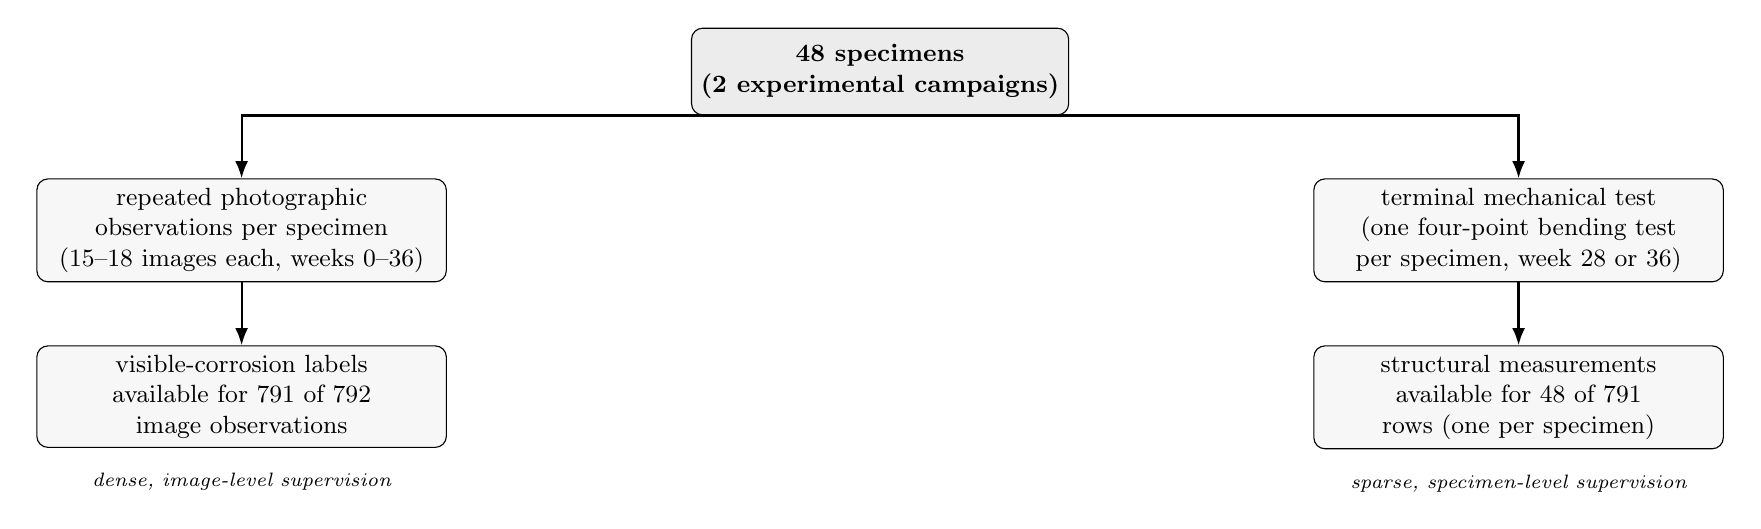
\begin{tikzpicture}[
    node distance=8mm and 14mm,
    box/.style={draw, rounded corners, align=center, minimum width=5.2cm,
                minimum height=1.1cm, font=\small, fill=gray!6},
    root/.style={draw, rounded corners, align=center, minimum width=4.2cm,
                minimum height=1.1cm, font=\small\bfseries, fill=gray!15},
    arr/.style={-{Latex[length=2.2mm]}, thick},
    lbl/.style={font=\scriptsize\itshape, align=center, text width=5.2cm}
]

\node[root] (root) {48 specimens\\(2 experimental campaigns)};

\node[box, below left=of root, xshift=-1.7cm] (imgs) {repeated photographic\\observations per specimen\\(15--18 images each, weeks 0--36)};
\node[box, below=of imgs] (corr) {visible-corrosion labels\\available for 791 of 792\\image observations};
\node[lbl, below=2mm of corr] (corrlbl) {dense, image-level supervision};

\node[box, below right=of root, xshift=1.7cm] (test) {terminal mechanical test\\(one four-point bending test\\per specimen, week 28 or 36)};
\node[box, below=of test] (struct) {structural measurements\\available for 48 of 791\\rows (one per specimen)};
\node[lbl, below=2mm of struct] (structlbl) {sparse, specimen-level supervision};

\draw[arr] (root.south) -| (imgs.north);
\draw[arr] (imgs) -- (corr);
\draw[arr] (root.south) -| (test.north);
\draw[arr] (test) -- (struct);

\end{tikzpicture}
}
\caption{Schematic contrast between dense, image-level visible-corrosion
supervision and sparse, specimen-level structural supervision, following
directly from Table~\ref{tab:quantity-availability}. This is a report
schematic illustrating the data structure described in
Sections~\ref{sec:data-modalities}--\ref{sec:structural-supervision}; it is
not a plot of experimental results.}
\label{fig:dataset-supervision-schematic}
\end{figure}

\section{Dataset Audit and Alignment}
\label{sec:dataset-audit}

The image archive contains 792 image files in total, spanning 48
specimens. Of these, one file — a single image belonging to a Campaign~2
specimen from the surface-inhibitor (spray) series — is corrupted and
cannot be decoded by standard image-reading routines. The remaining 791
files are readable and align to a corresponding metadata record.
Table~\ref{tab:dataset-overview} summarises the resulting dataset
dimensions on the aligned (791-row) basis that this report adopts by
default.

\begin{table}[htbp]
\centering
\caption{Dataset overview, aligned (791-row) basis, computed directly from
the current canonical dataset table.}
\label{tab:dataset-overview}
\begin{tabular}{ll}
\toprule
Quantity & Value \\
\midrule
Image files (raw archive) & 792 \\
Corrupted / unreadable image files & 1 \\
Aligned rows adopted by this report & 791 \\
Specimens & 48 \\
Experimental campaigns & 2 \\
Observation week range & 0--36 (irregular; 25 distinct week values) \\
Image observations per specimen & 15--18 (median 16) \\
Specimens with structural endpoint measurements & 48 of 48 (one
observation each) \\
\bottomrule
\end{tabular}
\end{table}

The project's own row-count convention for this one corrupted file has
evolved across its successive implementation phases, and this evolution
is best understood as a progressive tightening of data-quality policy
rather than as an unresolved inconsistency. Table~\ref{tab:corruption-handling}
summarises the three distinct policies adopted. The earliest exploratory
implementation removed the affected row from its working table without
substitution, arriving at 791 usable rows. The next three implementation
phases each instead retained all 792 rows and substituted the missing
image-derived quantities — handcrafted features in one phase, a learned
embedding in another, a broader interpretable feature set in a third —
with the corresponding column-wise median value, so that the corrupted
observation remained present but carried an imputed rather than a
measured image representation. The current and subsequent implementation
phases instead apply an explicit, configuration-level data-quality rule
that excludes any image that cannot be aligned to a readable, matched
record, which is the policy this report adopts by default: 791 aligned
rows drawn from 792 image files, 48 specimens.

\begin{table}[htbp]
\centering
\caption{Handling of the single corrupted image observation across
successive implementation phases, verified directly against each phase's
own data-loading code.}
\label{tab:corruption-handling}
\begin{tabular}{p{3.4cm}p{4.0cm}p{5.3cm}}
\toprule
Phase & Resulting row count & Handling mechanism \\
\midrule
Earliest exploratory implementation & 791 & Row silently omitted during
table construction; no substitution. \\
Classical baseline & 792 & Row retained; affected handcrafted image
features replaced by column-wise medians. \\
Deep-embedding phase & 792 & Row retained; affected learned image
embedding replaced by column-wise medians. \\
Interpretable multi-family feature phase & 792 & Row retained and flagged;
affected feature set (91 features) replaced by column-wise medians. \\
Current canonical phase (adopted here), inherited by the later
classification/augmentation effort & 791 & Row excluded by an explicit
alignment/readability policy prior to feature extraction. \\
\bottomrule
\end{tabular}
\end{table}

Because this row-count convention differs across phases, any quantitative
result drawn from an earlier phase and discussed later in this report
(Chapter~\ref{ch:activities}) is understood to be computed on a 792-row
basis with one imputed observation, whereas results drawn from the current
canonical phase and the later classification effort are computed on a
791-row aligned basis. The two bases are not row-for-row identical and are
not treated as interchangeable when results are compared
(Chapter~\ref{ch:results}).

A second, distinct schema change concerns the visible-corrosion severity
category labels introduced in Section~\ref{sec:data-modalities}. The
currently audited data table represents both the total-rust and peak-rust
severity categories on a four-level ordinal scale. An earlier canonical
dataset build, produced during the interpretable multi-family feature
phase on the historical 792-row basis, instead represented the same two
quantities on a five-level ordinal scale, with materially different class
counts (Table~\ref{tab:category-schema}). The data-loading code from that
earlier phase confirms the change directly: it is written to match a raw
workbook column defined over a five-level range, where the currently
audited workbook instead defines the corresponding column over a
four-level range. This is a genuine change in the underlying label schema
between the workbook snapshot used at that phase and the workbook snapshot
audited here, not a data-quality defect internal to the project, and the
two schemas are not treated as interchangeable in this report: a
categorical-classification result reported for the earlier phase in
Chapter~\ref{ch:activities} refers to a five-class problem and is not
described as an evaluation of the four-class scheme that the current
dataset, and the later classification and augmentation effort
(Section~\ref{sec:representation}, Chapter~\ref{ch:activities}), target.

\begin{table}[htbp]
\centering
\caption{Visible-corrosion severity category schema across dataset
builds. Class counts are ordered from the lowest to the highest severity
level.}
\label{tab:category-schema}
\begin{tabular}{p{4.2cm}p{2.1cm}p{3.1cm}p{3.1cm}}
\toprule
Dataset build & Row-count basis & Total-rust category counts & Peak-rust
category counts \\
\midrule
Interpretable multi-family feature phase (historical) & 792 (imputed) &
5 classes: 493 / 51 / 38 / 77 / 133 & 5 classes: 304 / 159 / 72 / 122 /
135 \\
Current canonical phase (audited; adopted by this report) & 791
(aligned) & 4 classes: 658 / 99 / 20 / 14 & 4 classes: 526 / 107 / 95 /
63 \\
\bottomrule
\end{tabular}
\end{table}

\section{Dataset Structure and Potential Confounding}
\label{sec:confounding}

Table~\ref{tab:campaign-design} shows that steel-mesh configuration,
chloride concentration, and terminal ageing duration do not vary
independently of campaign identity within the observed sample: every
specimen with the higher steel-mesh configuration also has the lower
chloride concentration and the shorter terminal ageing duration, and
belongs to Campaign~1; every specimen with the lower steel-mesh
configuration also has the higher chloride concentration and the longer
terminal ageing duration, and belongs to Campaign~2. No specimen in the
dataset combines a Campaign-1 mesh configuration with a Campaign-2
chloride level, or vice versa.

This structural property of the experimental design has a direct
consequence for how any statistical association between a design-linked
quantity and a measured outcome must be interpreted. Where an association
is estimated by pooling specimens across both campaigns, that association
cannot, on the evidence of the pooled sample alone, be uniquely attributed
to any one of the co-varying factors — campaign identity, mesh
configuration, chloride exposure, and ageing duration are, within this
sample, different labels for largely the same partition of specimens. A
pooled correlation involving one of these factors, or a quantity correlated
with one of them, should accordingly be read as a description of the
pooled sample rather than as evidence isolating the effect of that factor.
This report returns to the practical consequences of this property for
model evaluation in Chapters~\ref{ch:framework} and~\ref{ch:results}; the
present section deliberately stops short of discussing any modelling
result.

A related consequence concerns what it means to evaluate a model by
holding out an entire campaign. Because campaign identity coincides with a
specific combination of mesh configuration, chloride level, and ageing
duration, holding out one campaign does not test a model against unseen
specimens drawn from the same underlying design space as its training
data; it tests the model against specimens whose design characteristics
differ systematically, and simultaneously along several correlated
dimensions, from every specimen the model was trained on. Such an
evaluation is better characterised as a test of extrapolation across the
experimental design space than as an ordinary test of generalisation to
unseen specimens within that space. This distinction is developed formally
in Section~\ref{sec:eval-regimes}.

\section{Summary of Dataset Constraints}
\label{sec:dataset-summary}

The dataset available to this project is constrained in ways that
directly shape the modelling strategies described in later chapters:

\begin{itemize}
\item Visible-corrosion supervision is dense (available for 791 of 792
image observations) while structural supervision is sparse (available for
exactly 48 of those observations, one per specimen).
\item Repeated image observations of the same specimen are correlated, not
independent, and must be treated at the specimen level for evaluation
purposes.
\item No repeated or intermediate structural measurement exists for any
specimen; the dataset supports estimation of a single terminal structural
state per specimen, not a directly observed structural trajectory or
failure time.
\item Row-count and missing-observation conventions differ across the
project's implementation phases and must be stated explicitly whenever a
quantitative result is cited.
\item Campaign identity, steel-mesh configuration, chloride concentration,
and terminal ageing duration co-vary near-perfectly across the observed
specimens, limiting what can be inferred from pooled associations and
giving cross-campaign evaluation the character of extrapolation rather
than ordinary generalisation.
\end{itemize}

These constraints are the principal reason the project's modelling
strategy, described next in Chapter~\ref{ch:framework}, treats
specimen-level grouping, multiple evaluation regimes, and a conservative
distinction between measured, modelled, and derived-screening quantities
as required elements of the methodology rather than optional refinements.


% =============================================================
% Chapter 3 -- Common Methodological Framework
% =============================================================
\chapter{Common Methodological Framework}
\label{ch:framework}

Chapter~\ref{ch:dataset} established the structure and constraints of the
available data. This chapter describes the methodological framework that
the project's successive implementation phases used, with variation, to
work within those constraints. Rather than repeating a phase-by-phase
account here, it extracts the building blocks that recur across phases —
evaluation regimes, representation strategies, model families, metrics,
and the treatment of remaining-useful-life — so that
Chapter~\ref{ch:activities} can describe each phase's activity without
re-explaining shared machinery, and so that later comparisons
(Chapter~\ref{ch:results}) can be made on a consistent methodological
footing.

\section{General Modelling Philosophy}
\label{sec:philosophy}

The project's successive phases addressed several distinct prediction
problems over the same underlying dataset: estimating a specimen's current
visible-corrosion state from an image; predicting a specimen's terminal
structural condition; fitting an exploratory model of how corrosion and
structural condition evolve over time; screening for an approximate
service-life indicator; and, in a later and separate effort, classifying
images into a discrete visible-corrosion severity category. These are not
variations on a single problem, and the report does not treat them as such.

What is shared across phases is not the prediction target but a
methodological principle that later phases articulated increasingly
explicitly: a claim made about the data must correspond to the
supervision the data actually provides. A model trained on dense
visible-corrosion labels supports claims about visible-corrosion
estimation; it does not, by itself, support claims about structural
condition, service life, or failure risk, however plausible an
extrapolation from corrosion to those quantities might seem. The
distinctions drawn in Section~\ref{sec:dataset-summary} between directly
observed, model-derived, and derived-screening quantities are the
practical expression of this principle, and Section~\ref{sec:proxy-rul}
returns to its most consequential application.

\section{Leakage-Safe Specimen-Level Evaluation}
\label{sec:leakage}

Section~\ref{sec:longitudinal} established that the repeated image
observations of a given specimen are correlated rather than independent.
This has a direct and easily overlooked consequence for evaluation.

Consider a dataset of image observations split into training and test
partitions by assigning individual image rows at random, without regard
to which specimen each row belongs to. Because a typical specimen
contributes fifteen to eighteen images spanning its entire observation
period, a random row-wise split will, with high probability, place most
of a given specimen's images in the training partition and a few of the
same specimen's images in the test partition. A model evaluated in this
way can achieve a low test error not by learning corrosion cues that
generalise to specimens it has never seen, but by learning to recognise
that specific specimen — its particular lighting, its particular
background, or idiosyncrasies of its individual corrosion pattern — from
the many other images of it already seen in training. The resulting test
error understates the error the same model would incur on a genuinely
unseen specimen, and the extent of this understatement is not visible from
the row-wise test score alone.

The project's later implementation phases addressed this by grouping
observations at the specimen level before splitting: every image
belonging to a given specimen is assigned to the same partition, so that a
specimen appearing in the test partition never also appears in training.
Figure~\ref{fig:specimen-splitting} contrasts the two approaches. This
grouping principle is applied consistently, regardless of which of the
three evaluation regimes described next is used to decide which specimens
are held out.

\begin{figure}[htbp]
\centering
\resizebox{0.75\textwidth}{!}{% Report schematic (not an experimental result).
% Contrasts a naive row-wise random split of image observations against
% a specimen-level grouped split, for four illustrative specimens A-D
% each with several repeated image observations.
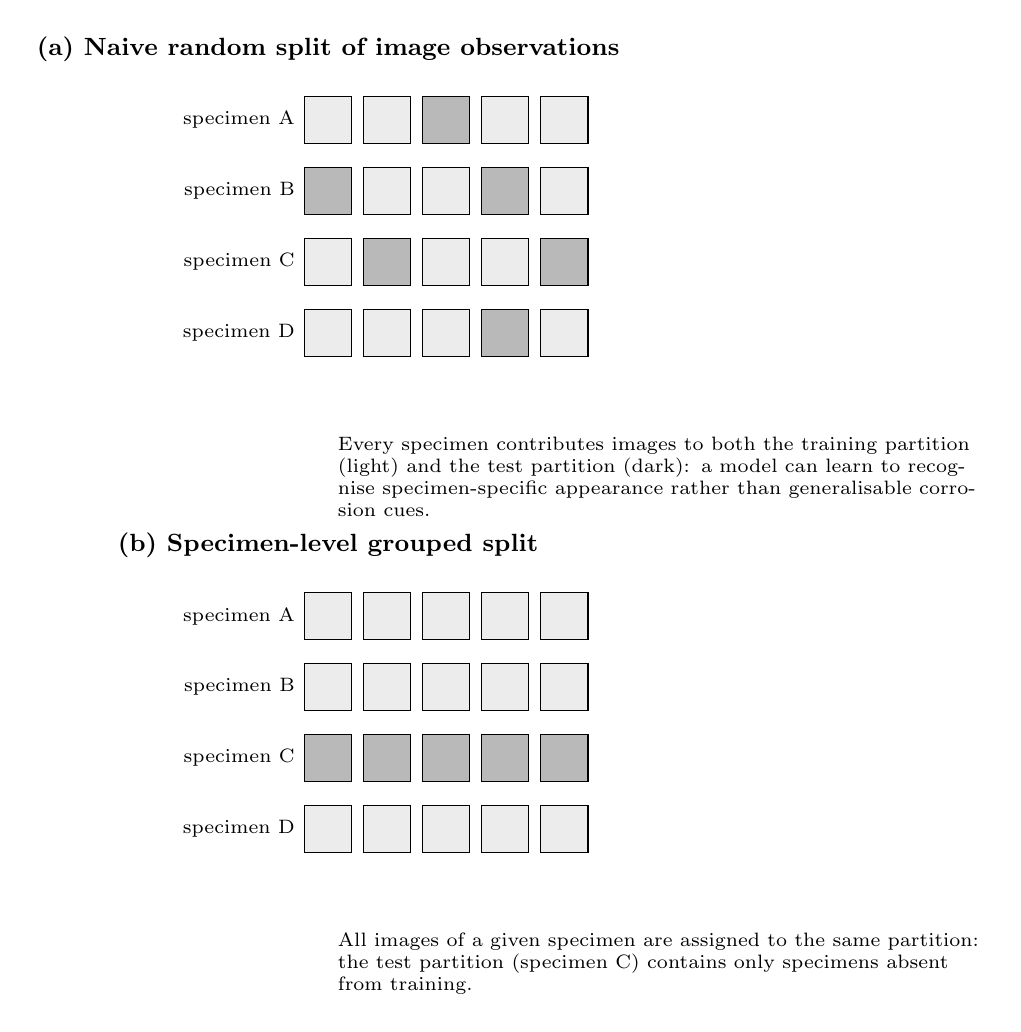
\begin{tikzpicture}[
    sq/.style={draw, minimum size=6mm, inner sep=0pt, font=\tiny},
    train/.style={sq, fill=gray!15},
    test/.style={sq, fill=gray!55},
    lbl/.style={font=\scriptsize, anchor=east},
    panelcap/.style={font=\small\bfseries}
]

% --- Panel (a): naive random row-wise split ---
\node[panelcap] at (0,0) {(a) Naive random split of image observations};

\foreach \row/\name/\pattern [count=\r from 0] in
    {0/A/{train,train,test,train,train},
     1/B/{test,train,train,test,train},
     2/C/{train,test,train,train,test},
     3/D/{train,train,train,test,train}} {
    \node[lbl] at (-0.3,-0.9-\r*0.9) {specimen \name};
    \foreach \p [count=\c from 0] in \pattern {
        \node[\p] at (\c*0.75,-0.9-\r*0.9) {};
    }
}
\node[font=\scriptsize, align=left, text width=8.2cm, anchor=north west]
    at (0,-4.8) {Every specimen contributes images to both the training
    partition (light) and the test partition (dark): a model can learn to
    recognise specimen-specific appearance rather than generalisable
    corrosion cues.};

% --- Panel (b): specimen-level grouped split ---
\begin{scope}[yshift=-6.3cm]
\node[panelcap] at (0,0) {(b) Specimen-level grouped split};

\foreach \row/\name/\assign [count=\r from 0] in
    {0/A/train,1/B/train,2/C/test,3/D/train} {
    \node[lbl] at (-0.3,-0.9-\r*0.9) {specimen \name};
    \foreach \c in {0,...,4} {
        \node[\assign] at (\c*0.75,-0.9-\r*0.9) {};
    }
}
\node[font=\scriptsize, align=left, text width=8.2cm, anchor=north west]
    at (0,-4.8) {All images of a given specimen are assigned to the same
    partition: the test partition (specimen C) contains only specimens
    absent from training.};
\end{scope}

\end{tikzpicture}
}
\caption{Report schematic contrasting a naive row-wise random split, which
can place images of the same specimen on both sides of a train/test
partition, against a specimen-level grouped split, which cannot. Not an
experimental result.}
\label{fig:specimen-splitting}
\end{figure}

\section{Evaluation Regimes}
\label{sec:eval-regimes}

Specimen-level grouping determines that whole specimens, not individual
images, are the unit of assignment to a partition. It does not by itself
determine \emph{which} specimens are held out, or what question the
resulting evaluation answers. The project uses three distinct regimes for
this purpose, each targeting a different question, summarised in
Table~\ref{tab:eval-regimes} and illustrated schematically in
Figure~\ref{fig:eval-regimes}.

\subsection{Grouped specimen holdout}
\label{sec:grouped-holdout}

A random subset of specimens is held out from the pooled observed dataset
without deliberately withholding an entire treatment or campaign. It
therefore provides an interpolation-oriented unseen-specimen evaluation,
answering the question of how well a model generalises to specimens it
has not seen, drawn at random from the same pooled experimental mixture
it was trained on. This is distinct from stratified sampling: because the
subset is drawn at random rather than balanced by design, individual
folds may be imbalanced in campaign or treatment composition and need not
contain every subgroup. It is the regime closest to ordinary interpolation
within the observed design space, and, where repeated evaluation is used,
results are averaged over multiple random selections of the held-out
subset.

\subsection{Leave-one-treatment-out}
\label{sec:loto}

All specimens sharing a given treatment protocol are held out together,
cycling over the available treatment groups so that every group is used
as the test partition exactly once. This answers a more demanding
question: whether a model's predictions transfer to a treatment protocol
it has never encountered at all, rather than merely to unseen specimens of
protocols it has already seen examples of. Because some treatment groups
are represented by very few specimens (Table~\ref{tab:campaign-design}),
individual leave-one-treatment-out folds can be based on small held-out
samples, and results for the smallest groups are correspondingly less
stable.

\subsection{Leave-one-campaign-out}
\label{sec:loco}

All specimens belonging to one full experimental campaign are held out,
and the model is trained on the other campaign alone. This is the
strongest distribution shift the dataset can express, since, as
established in Section~\ref{sec:confounding}, campaign identity coincides
with a specific combination of steel-mesh configuration, chloride
concentration, and terminal ageing duration. A model evaluated under
leave-one-campaign-out is therefore not being tested on specimens drawn
from the training distribution; it is being tested on specimens whose
design characteristics differ systematically, along several correlated
dimensions at once, from every specimen available for training. For this
reason, leave-one-campaign-out performance in this dataset should not be
read as an estimate of expected performance on future, similarly-designed
specimens; it is better understood as a stress test of extrapolation
across the experimental design space, and the two readings can differ
substantially. This report does not present leave-one-campaign-out results
in this chapter — the regime is defined here only as a methodological
tool; its results, and what they imply, are discussed once the relevant
modelling activities are described in Chapters~\ref{ch:activities}
and~\ref{ch:results}.

\begin{table}[htbp]
\centering
\caption{The three specimen-level evaluation regimes used across the
project, and the question each is designed to answer.}
\label{tab:eval-regimes}
\begin{tabular}{p{3.6cm}p{3.6cm}p{6.2cm}}
\toprule
Regime & Held-out unit & Question answered \\
\midrule
Grouped specimen holdout & Random subset of specimens & Generalisation to
unseen specimens drawn from the same observed experimental mixture. \\
Leave-one-treatment-out & All specimens of one treatment protocol & Transfer
to a treatment protocol not seen at all during training. \\
Leave-one-campaign-out & All specimens of one full campaign & Robustness
under the strongest available distribution shift; partly an extrapolation
test across correlated design variables (Section~\ref{sec:confounding}). \\
\bottomrule
\end{tabular}
\end{table}

\begin{figure}[htbp]
\centering
\resizebox{0.8\textwidth}{!}{% Report schematic (not an experimental result).
% Illustrates, for a generic grid of specimens organised by campaign
% (rows) and treatment group (columns), which specimens are held out
% as the test partition under each of the three evaluation regimes.
% The layout is illustrative only and does not reproduce the exact
% campaign/treatment specimen counts given in the dataset chapter.
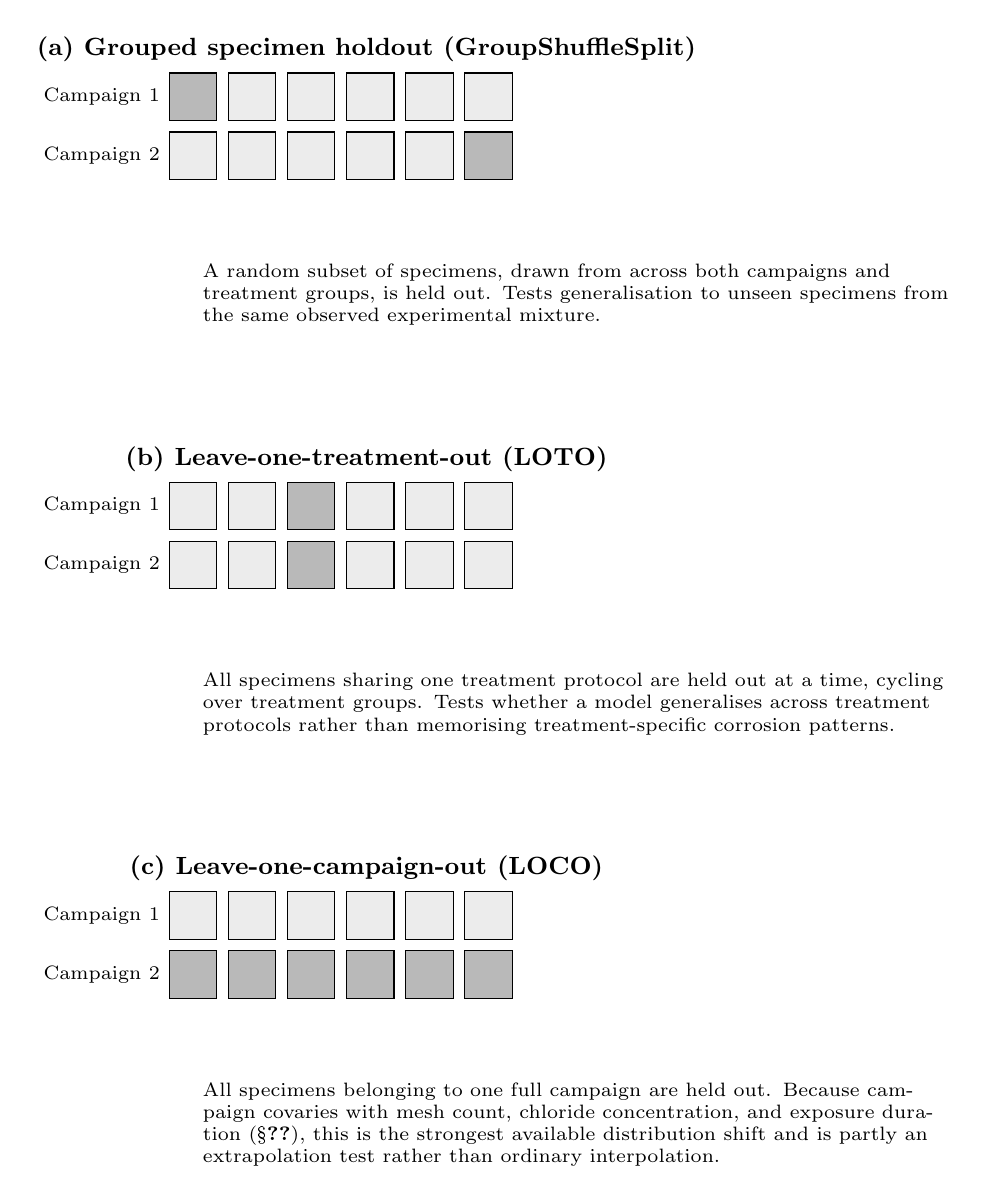
\begin{tikzpicture}[
    sq/.style={draw, minimum size=6mm, inner sep=0pt},
    train/.style={sq, fill=gray!15},
    held/.style={sq, fill=gray!55},
    panelcap/.style={font=\small\bfseries},
    rlbl/.style={font=\scriptsize, anchor=east},
    clbl/.style={font=\scriptsize, anchor=south}
]

\def\ncols{6}

% --- Panel (a): GroupShuffleSplit ---
\node[panelcap] at (2.2,0.6) {(a) Grouped specimen holdout (GroupShuffleSplit)};
\foreach \r/\rowname in {0/Campaign 1, 1/Campaign 2} {
    \node[rlbl] at (-0.3,-\r*0.75) {\rowname};
    \foreach \c in {0,...,5} {
        \pgfmathtruncatemacro{\isheld}{mod(\c+2*\r,7)==0}
        \ifnum\isheld=1
            \node[held] at (\c*0.75,-\r*0.75) {};
        \else
            \node[train] at (\c*0.75,-\r*0.75) {};
        \fi
    }
}
\node[font=\scriptsize, align=left, text width=9.5cm, anchor=north west]
    at (0,-2.0) {A random subset of specimens, drawn from across both
    campaigns and treatment groups, is held out. Tests generalisation
    to unseen specimens from the same observed experimental mixture.};

% --- Panel (b): LOTO ---
\begin{scope}[yshift=-5.2cm]
\node[panelcap] at (2.2,0.6) {(b) Leave-one-treatment-out (LOTO)};
\foreach \r/\rowname in {0/Campaign 1, 1/Campaign 2} {
    \node[rlbl] at (-0.3,-\r*0.75) {\rowname};
    \foreach \c in {0,...,5} {
        \ifnum\c=2
            \node[held] at (\c*0.75,-\r*0.75) {};
        \else
            \node[train] at (\c*0.75,-\r*0.75) {};
        \fi
    }
}
\node[font=\scriptsize, align=left, text width=9.5cm, anchor=north west]
    at (0,-2.0) {All specimens sharing one treatment protocol are held
    out at a time, cycling over treatment groups. Tests whether a model
    generalises across treatment protocols rather than memorising
    treatment-specific corrosion patterns.};
\end{scope}

% --- Panel (c): LOCO ---
\begin{scope}[yshift=-10.4cm]
\node[panelcap] at (2.2,0.6) {(c) Leave-one-campaign-out (LOCO)};
\foreach \r/\rowname in {0/Campaign 1, 1/Campaign 2} {
    \node[rlbl] at (-0.3,-\r*0.75) {\rowname};
    \foreach \c in {0,...,5} {
        \ifnum\r=1
            \node[held] at (\c*0.75,-\r*0.75) {};
        \else
            \node[train] at (\c*0.75,-\r*0.75) {};
        \fi
    }
}
\node[font=\scriptsize, align=left, text width=9.5cm, anchor=north west]
    at (0,-2.0) {All specimens belonging to one full campaign are held
    out. Because campaign covaries with mesh count, chloride
    concentration, and exposure duration (\S\ref{sec:confounding}), this
    is the strongest available distribution shift and is partly an
    extrapolation test rather than ordinary interpolation.};
\end{scope}

\end{tikzpicture}
}
\caption{Report schematic of the three evaluation regimes, for an
illustrative grid of specimens organised by campaign and treatment group.
Held-out (test) specimens are shown in the darker shade. The layout is
illustrative and does not reproduce the exact specimen counts of
Table~\ref{tab:campaign-design}.}
\label{fig:eval-regimes}
\end{figure}

\section{Image Representation Strategies}
\label{sec:representation}

Across its successive phases, the project explored five broad strategies
for converting an image observation into a representation usable by a
predictive model:

\begin{enumerate}
\item[A.] \textbf{Threshold and handcrafted colour descriptors.} A small
number of scalar quantities computed from fixed colour-space thresholds
(for example, the proportion of pixels falling within a rust-coloured
range), used by the earliest implementation phases.
\item[B.] \textbf{Pretrained deep embeddings.} A fixed-length vector
representation obtained by passing each image through a convolutional
network pretrained on a large natural-image dataset and used as a frozen
feature extractor, without further training of the network itself.
\item[C.] \textbf{Interpretable multi-family features.} A broader,
explicitly engineered set of descriptors spanning colour, texture, surface
morphology, and spatial location of corrosion along the specimen, designed
so that each feature has a stated physical or visual interpretation.
\item[D.] \textbf{RGB/HSV summary representations.} Colour-space summary
statistics computed in both RGB and HSV representations, introduced
specifically to test whether a compact, interpretable colour description
adds value once specimen-design metadata is already available, in the
project's terminal-load-focused analysis.
\item[E.] \textbf{Raw-image deep classification (planned).} Direct
classification of raw images into a discrete corrosion-severity category
using a deep image classifier, which is the intended representation
strategy for the later four-class classification effort described in
Chapter~\ref{ch:activities}; at the time of writing, this strategy has been
prepared for (through a dedicated, leakage-safe data and augmentation
pipeline) but not yet trained or evaluated.
\end{enumerate}

These strategies are introduced here only as a taxonomy; the specific
feature definitions used within each strategy are not repeated in this
chapter and, where needed for reference, are catalogued in an appendix.

\section{Metadata and Multimodal Inputs}
\label{sec:multimodal}

A recurring methodological question across phases is whether an
image-derived representation, of any of the strategies above, contributes
predictive information beyond what is already available from specimen and
exposure metadata (Table~\ref{tab:campaign-design}) alone. This question
matters because metadata and image-derived quantities are not, in
general, independent sources of information in this dataset: a specimen's
treatment and campaign membership can itself be predictive of its
corrosion appearance or its structural condition, independently of
whatever a photograph of it shows.

The project's treatment of this question was not uniform across phases,
and the framework below describes how the comparison was eventually
formalised rather than a design followed from the outset. The
deep-embedding phase compared an image-only configuration against a
combined image-plus-metadata configuration, but did not include a
comparable metadata-only baseline alongside them. It was the later
terminal-load-focused work that made an explicit three-way comparison —
an \emph{image-only} configuration using an image representation without
metadata, a \emph{metadata-only} configuration using specimen and exposure
design variables without any image-derived quantity, and a
\emph{combined} (multimodal) configuration using both together — a
central and consistently applied part of its methodology. Where this
three-way comparison is available, it is the project's principal tool for
distinguishing predictive value that is genuinely attributable to the
visual appearance of corrosion from predictive value that is instead
attributable to the specimen's known design and exposure conditions; where
only the narrower two-way comparison is available, this is stated
explicitly alongside the corresponding result. The outcomes of these
comparisons, for the phases in which they were carried out, are reported
in Chapters~\ref{ch:activities} and~\ref{ch:results}.

\section{Model Families}
\label{sec:model-families}

Table~\ref{tab:model-families} lists the model families used across the
project's phases. The choice of family in each phase was pragmatic rather
than exploratory: regularised linear regression provides an
interpretable, low-variance baseline that is particularly informative
when the training sample is small (as it is for the structural targets,
Section~\ref{sec:structural-supervision}); tree-ensemble methods
(Random Forest, Gradient Boosting, XGBoost, CatBoost) provide stronger
non-linear fits with built-in feature-importance diagnostics; a small
multilayer perceptron was used to combine a fixed-length embedding with
tabular metadata; a pretrained convolutional network provided image
embeddings as described in Section~\ref{sec:representation}; and a small
family of parametric and non-parametric curve models was used specifically
to fit specimen-level degradation trajectories over time
(Section~\ref{sec:proxy-rul}). This chapter does not develop the
mathematical detail of any of these families; it records only their role
in the project.

\begin{table}[htbp]
\centering
\caption{Model families used across the project, and their role.}
\label{tab:model-families}
\begin{tabular}{p{4.3cm}p{8.9cm}}
\toprule
Family & Role in the project \\
\midrule
Ridge / linear regression & Regularised, low-variance baseline;
particularly relevant given the small number of structural observations. \\
Random Forest & Non-linear regression and classification baseline with
feature-importance diagnostics; used across most phases and targets. \\
Gradient Boosting & Alternative non-linear ensemble, compared against
Random Forest per task. \\
XGBoost & Alternative gradient-boosted ensemble, benchmarked in the
earliest classical phase and again, alongside other candidate families,
in the later terminal-load-focused modelling. \\
CatBoost & Additional gradient-boosted ensemble candidate introduced in
later structural-condition modelling; used with the same numeric feature
tables as the other ensemble methods, not configured to use its native
categorical-feature handling. \\
Multilayer perceptron (MLP) & Combines a fixed-length image embedding
with tabular metadata; also used as an image-only regressor for
comparison. \\
Pretrained convolutional network & Frozen (not fine-tuned) feature
extractor producing the fixed-length image embedding consumed by the
MLP above. \\
Degradation-curve models & A small family of parametric (linear,
logarithmic, logistic, Gompertz) and non-parametric (monotone-isotonic)
curves fitted to estimated condition over the observation period, as
input to the proxy-RUL computation (Section~\ref{sec:proxy-rul}). \\
\bottomrule
\end{tabular}
\end{table}

\section{Evaluation Metrics}
\label{sec:metrics}

Model performance is reported using a small, consistent set of metrics,
defined here so that later chapters can use them without redefinition.
For regression targets, the project reports the mean absolute error (MAE)
and root-mean-square error (RMSE), both in the physical units of the
target; the coefficient of determination ($R^2$); and the Spearman rank
correlation between predicted and observed values. For the four-class
classification target, the project's planned evaluation (not yet carried
out; Section~\ref{sec:representation}, strategy~E) specifies overall
accuracy, macro-averaged F1 score, and per-class recall reported through a
confusion matrix.

Spearman rank correlation is reported alongside the absolute-error metrics
because it evaluates whether a model correctly orders specimens by
severity without requiring its predictions to be correctly scaled or
calibrated in absolute terms, and because it is markedly less sensitive
than MAE or RMSE to a small number of specimens with large absolute
errors. A model can be poorly calibrated in absolute magnitude while still
correctly identifying which specimens are more severely affected than
others, and the two metrics together distinguish this situation from one
in which a model's ranking of specimens is itself unreliable.

Macro-averaged F1, rather than overall accuracy, is identified in advance
as the primary metric for the planned four-class classification task
because the four severity classes are markedly imbalanced in the
underlying data (Table~\ref{tab:data-modalities}): the lowest-severity
class accounts for the large majority of observations. A classifier that
predicted the majority class for every observation would achieve high
overall accuracy while providing no discrimination among the
minority, higher-severity classes that are of greatest practical
interest. Macro-averaged F1 weights each class equally regardless of its
frequency and is therefore markedly more informative than accuracy alone
for this task; per-class recall and the confusion matrix are reported
alongside it to characterise which classes, specifically, a classifier
confuses.

\section{True Remaining-Useful-Life versus Proxy-RUL}
\label{sec:proxy-rul}

This section states explicitly a methodological boundary that governs
every subsequent discussion of service-life or degradation in this
report.

The dataset, as established in Section~\ref{sec:structural-supervision},
does not contain the supervision required to train a model to predict
remaining useful life, or time to failure, in the ordinary supervised
sense. Such a target would require either a recorded failure event time
for each specimen or repeated structural measurements of the same
specimen at multiple points in time, so that the rate and trajectory of
structural degradation could be observed directly. Neither is present:
each specimen contributes a single terminal structural measurement, taken
once, at the end of its observation period, and no specimen is observed to
fail during a monitored period with the failure time recorded.

In place of a directly supervised target, later project phases constructed
a screening-oriented proxy through an explicit, multi-step derivation:

\begin{enumerate}
\item A model trained on the available (dense, visible-corrosion or
metadata-linked) supervision produces an \emph{estimated} structural or
corrosion condition at each observation week for a given specimen,
including weeks at which no direct measurement exists.
\item These estimated, per-week values are used to fit a specimen-level
degradation curve over the observation period, using one of the curve
families listed in Table~\ref{tab:model-families}.
\item An engineering threshold is defined on the quantity described by
that curve (for example, a specified level of estimated wire-area loss).
\item The time at which the fitted curve is projected to cross that
threshold, measured forward from the specimen's last available
observation, is reported as the proxy remaining-useful-life.
\end{enumerate}

Every step in this derivation is model-dependent: it depends on the
accuracy of the condition estimates produced in step 1, on the curve
family selected in step 2, and on the threshold chosen in step 3. None of
these choices is fixed by direct observation. The resulting quantity is
therefore an exploratory, screening-oriented output, useful for
prioritising which specimens might warrant closer inspection, and it is
not, and should not be presented as, an observed or directly supervised
lifetime measurement. This report consistently uses the qualified term
\emph{proxy-RUL} for this quantity and reserves \emph{remaining useful
life} or \emph{RUL} without qualification for a genuinely observed
lifetime target, which this dataset does not provide.

\section{Methodological Principles Carried Forward}
\label{sec:principles}

Not every phase of the project met the standards described in this
chapter: the earliest exploratory prototype, in particular, did not
evaluate its production model against any held-out partition at all, and
Chapter~\ref{ch:activities} reports this and other historical shortcomings
where they occurred rather than treating this chapter's framework as
retroactively true of every prior phase. The principles below instead
describe the position reached by the project's mature pipeline — the
implementation phases responsible for the majority of the results
discussed in Chapters~\ref{ch:activities} and~\ref{ch:results} — and are
adopted in this report as the standard against which a result is judged to
constitute valid evidence. Where an earlier or partial phase departs from
one of these principles, that departure is noted explicitly at the point
the result is discussed, rather than silently overlooked or silently
corrected:

\begin{itemize}
\item Evaluation is grouped at the specimen level; a result is not treated
as valid evidence of generalisation if it comes from a split that places
images of the same specimen in both training and test partitions.
\item Wherever an image-derived representation is proposed as predictive
of an outcome, its contribution is, from the terminal-load-focused phase
onward, checked against an explicit image-only, metadata-only, and
combined comparison; earlier phases that instead compared only two of
these three configurations are identified as such (Section~\ref{sec:multimodal}).
\item Model robustness is preferably assessed under more than one
evaluation regime, including at least one regime designed to expose
distribution shift (leave-one-treatment-out or leave-one-campaign-out),
rather than reported under a single grouped holdout alone.
\item Observed quantities, model-derived quantities, and derived-screening
quantities (Table~\ref{tab:quantity-availability}) are kept terminologically
distinct throughout this report, and a derived-screening output is never
described in language implying it is a direct measurement or a supervised
prediction of an observed target.
\item Proxy-RUL outputs are interpreted conservatively, as exploratory
screening indicators contingent on the modelling choices used to derive
them, not as validated lifetime estimates.
\item Where a directly measured endpoint is available for a quantity of
interest, the project's later work favours modelling that endpoint
directly over constructing a further derived proxy for it.
\end{itemize}


% =============================================================
% Chapter 4 -- Research and Development Activities
% (Sections 4.1-4.4 only in this pass; 4.5 onward not yet written)
% =============================================================
\chapter{Research and Development Activities}
\label{ch:activities}

This chapter reconstructs the project as a chronological scientific and
engineering investigation. Each section addresses one implementation phase in
turn, but the organising logic is not "what was built" so much as: what
question the phase was trying to answer, what the resulting evidence showed,
what limitation that evidence exposed, and what decision followed from it.
Provenance labels for each phase are given only in footnotes and figure/table
captions, where they matter for traceability; the prose refers to phases by
their scientific role. The shared methodological vocabulary — specimen-level
grouping, the three evaluation regimes, the representation-strategy taxonomy,
and the distinction between observed, model-derived, and derived-screening
quantities — was established in Chapter~\ref{ch:framework} and is used here
without re-derivation.

\section{Exploratory Prototype}
\label{sec:phase0}

The project's first implementation was an informal exploratory prototype,
built to establish whether the available photographs contained any usable
signal at all rather than to produce a validated model.\footnote{Corresponds
to the earliest exploratory implementation referenced in Chapter~\ref{ch:dataset}'s
corrupted-image-handling table.} It computed a single fixed-threshold
colour mask per image, derived a handful of additional descriptors by parsing
the specimen identifier as a string (rather than reading the structured
metadata table), and trained a RandomForest to predict next-week visible rust
percentage. A separate script then applied this one-step regressor
autoregressively — repeatedly feeding each week's prediction back in as the
next week's input — until a fixed 10\% rust threshold was crossed, and
reported the number of simulated steps as a "remaining useful life."

This should not be read as a trained or validated RUL model: it is a
heuristic simulation built on a single-step regressor, compounding that
regressor's error at every simulated step, with no mechanism to check the
simulated trajectory against an observed one. More consequentially, the
script that produces the prototype's "production" model fits on the entire
available dataset with no held-out partition at all, and no metrics from
this phase were saved anywhere in the repository — every quantitative claim
about this phase's performance would have to come from console output that
no longer exists. The phase is therefore useful only as a starting point: it
suggested that a colour-based signal was worth pursuing, while simultaneously
demonstrating that a benchmarked, leakage-aware, and reproducible pipeline
did not yet exist. That gap is what the next phase was built to close.

\section{Classical Machine-Learning Baseline}
\label{sec:phase1}

The second phase replaced the prototype with a benchmarked pipeline: a
consistent set of candidate regressors (ElasticNet, RandomForest, Gradient
Boosting, and XGBoost) evaluated under a specimen-grouped holdout followed by
grouped cross-validation on the training partition, with metrics and feature
importances persisted for every candidate. Rather than posing one prediction
problem, the phase implemented three distinct tasks over the same
underlying data, distinguished here because they have different scientific
meanings and must not be merged.

\textbf{Current visible-corrosion estimation} predicted the current-week peak
rust percentage from a combination of handcrafted image descriptors and
specimen/exposure metadata. The selected RandomForest achieved a grouped
holdout MAE of 2.38 and $R^2 = 0.900$ — the strongest headline number produced
by this phase. Inspecting the model's own feature importances, however,
shows that a single handcrafted feature — the percentage of pixels falling
inside a fixed rust-colour threshold — accounts for over 90\% of the total
importance. Because this same colour threshold is also how the target label
itself is effectively derived, the result is close to a restatement of the
labelling rule rather than independent evidence that the model has learned a
generalisable visual concept of corrosion. The headline accuracy is real, but
it does not by itself establish that the model has captured visual
information beyond the threshold used to construct its own label.

\textbf{Progression modelling} predicted the same current-week rust target
from specimen/exposure metadata and observation week alone, with no image
input at all. This is a metadata- and week-conditioned regression, not a
sequence model: it does not consume a specimen's own history of prior
observations and does not forecast forward from one time step to the next.
The selected Gradient Boosting model reached a grouped holdout $R^2$ of only
0.517, substantially weaker than the image-assisted task above, and the
result should be read accordingly — as an estimate of how much predictive
information design and exposure variables alone carry for this target,
not as a temporal forecasting result.

\textbf{Threshold-timing estimation} predicted the number of weeks remaining
until peak rust crosses a fixed 20\% threshold, using the specimen's true
current corrosion level (not a model's own prediction of it) together with
metadata as inputs. The selected RandomForest reached a grouped holdout MAE
of 2.21 weeks. This is a derived timing quantity conditioned on an observed
covariate, not an instance of remaining-useful-life prediction in the sense
defined in Section~\ref{sec:proxy-rul}: it times a corrosion threshold, not a
structural failure or service-life endpoint, and it is trained on already
known rather than forecast inputs.

\begin{table}[htbp]
\centering
\caption{Representative grouped-holdout results, classical baseline phase.
Selected model and holdout metrics as saved by the phase's own evaluation
script.}
\label{tab:phase1-results}
\begin{tabular}{p{4.3cm}p{2.6cm}p{1.5cm}p{1.6cm}p{1.5cm}}
\toprule
Task & Selected model & MAE & RMSE & $R^2$ \\
\midrule
Current corrosion (image + metadata) & RandomForest & 2.38 & 4.25 & 0.900 \\
Progression (metadata + week only) & Gradient Boosting & 6.71 & 9.33 & 0.517 \\
Threshold-timing (weeks to 20\%) & RandomForest & 2.21 wk & 3.09 wk & 0.782 \\
\bottomrule
\end{tabular}
\end{table}

Two further findings from this phase materially affect how its results
should be read. First, the specimen-grouped holdout used throughout this
phase was a genuine improvement over the exploratory prototype's absence of
any held-out evaluation, and is the same grouping principle formalised in
Section~\ref{sec:leakage}. Second, model selection within each task was
based on the holdout metric itself rather than on a separate validation
partition: for the threshold-timing task, an alternative candidate achieves
a better holdout RMSE (2.82 vs.\ 3.09) and $R^2$ (0.818 vs.\ 0.782) than the
selected RandomForest, which is chosen because its holdout MAE is
marginally lower (2.21 vs.\ 2.24). This is a historical model-selection
practice specific to this phase, not the methodological standard adopted
later in the project (Section~\ref{sec:principles}), and it means the
reported holdout numbers should be read as an optimistic upper bound on
this phase's true generalisation performance rather than as an untouched
final estimate. The pipeline's reproducibility is also limited in the
current repository state: re-running it against the presently stored data
workbook raises a schema mismatch, so the numbers above are the saved
record of a historical run rather than a result that can be freshly
regenerated without repair.

Taken together, the phase established that a benchmarked, specimen-grouped
pipeline could produce strong-looking results for current-corrosion
estimation, but left open whether that strength reflected a genuinely useful
image representation or simply a restatement of the handcrafted threshold
used to build the label. Testing whether a representation learned directly
from image content, rather than a fixed hand-designed threshold, could
resolve this question motivated the next phase.

\section{Deep Image-Embedding Experiment}
\label{sec:phase2}

The third phase replaced the handcrafted colour threshold with a
representation learned by a convolutional network: each image was passed
through a pretrained ImageNet ResNet-18 with its final classification layer
removed, used purely as a frozen feature extractor (no weights in the
backbone were updated), producing a 512-dimensional embedding. The
experiment targeted the same family of quantity as the previous phase's
strongest result — current-week peak rust percentage — so that the value of
a learned representation could be assessed against a comparable target,
computed here on the phase's own 792-row dataset basis, with the one
corrupted image's embedding replaced by the column-wise median.

Two configurations were compared: an image-only regressor consuming only the
512-dimensional embedding, and a multimodal regressor consuming the same
embedding concatenated with seven metadata fields. No metadata-only baseline
was trained in this phase, so the comparison that later became central to
the project's methodology (Section~\ref{sec:multimodal}) is only partially
available here.

The results contain a genuine reversal worth stating clearly.
Across training, the multimodal model reached a lower best validation MAE
than the image-only model (4.02 vs.\ 4.96). On the held-out test partition,
however, the ranking inverted: the image-only model achieved a lower test
MAE than the multimodal model (5.63 vs.\ 5.75). Figure~\ref{fig:phase2-fusion}
shows both comparisons side by side. The phase's own pipeline selected the
final deployed model by test MAE — the same partition used to report the
final metric — so the image-only model was deployed on the strength of a
test-set comparison that also served as the reported result, rather than
being confirmed by an independent partition after selection. This mirrors
the model-selection pattern already noted in Section~\ref{sec:phase1} and
should likewise be read as a historical practice specific to this phase,
not a result that establishes multimodal fusion as inferior in general.

\begin{figure}[htbp]
\centering
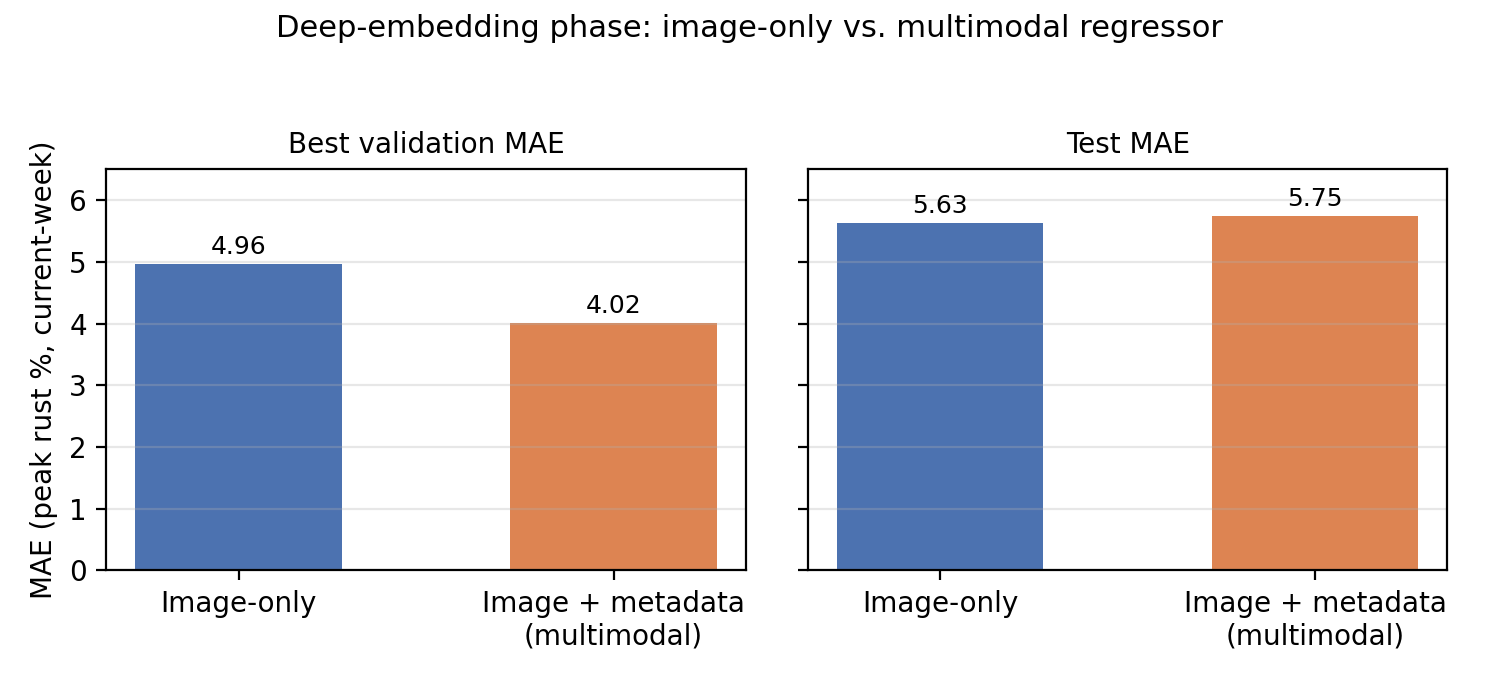
\includegraphics[width=0.85\textwidth]{fig_4_1_main2_image_only_vs_multimodal.png}
\caption{Deep-embedding phase: best validation MAE versus test MAE for the
image-only and multimodal (image + metadata) regressors, current-week peak
rust percentage. The multimodal model is ahead on validation but behind on
test; the deployed model was chosen by the test-partition comparison shown
on the right. Generated from the phase's own saved training history and
model-comparison tables.}
\label{fig:phase2-fusion}
\end{figure}

A second finding concerns where the deployed model's errors concentrate.
Grouping the saved test-set residuals by observation week shows a
systematic pattern: mean absolute error rises from 2.22 at week 10 or
earlier, to 6.62 across weeks 12–20, to 12.08 from week 23 onward, and the
average bias moves from a small positive value ($+0.85$) to a substantial
negative one ($-6.91$) over the same progression. Figure~\ref{fig:phase2-residuals}
shows this directly: the model increasingly underestimates severity as
corrosion advances, rather than erring in either direction at random.

\begin{figure}[htbp]
\centering
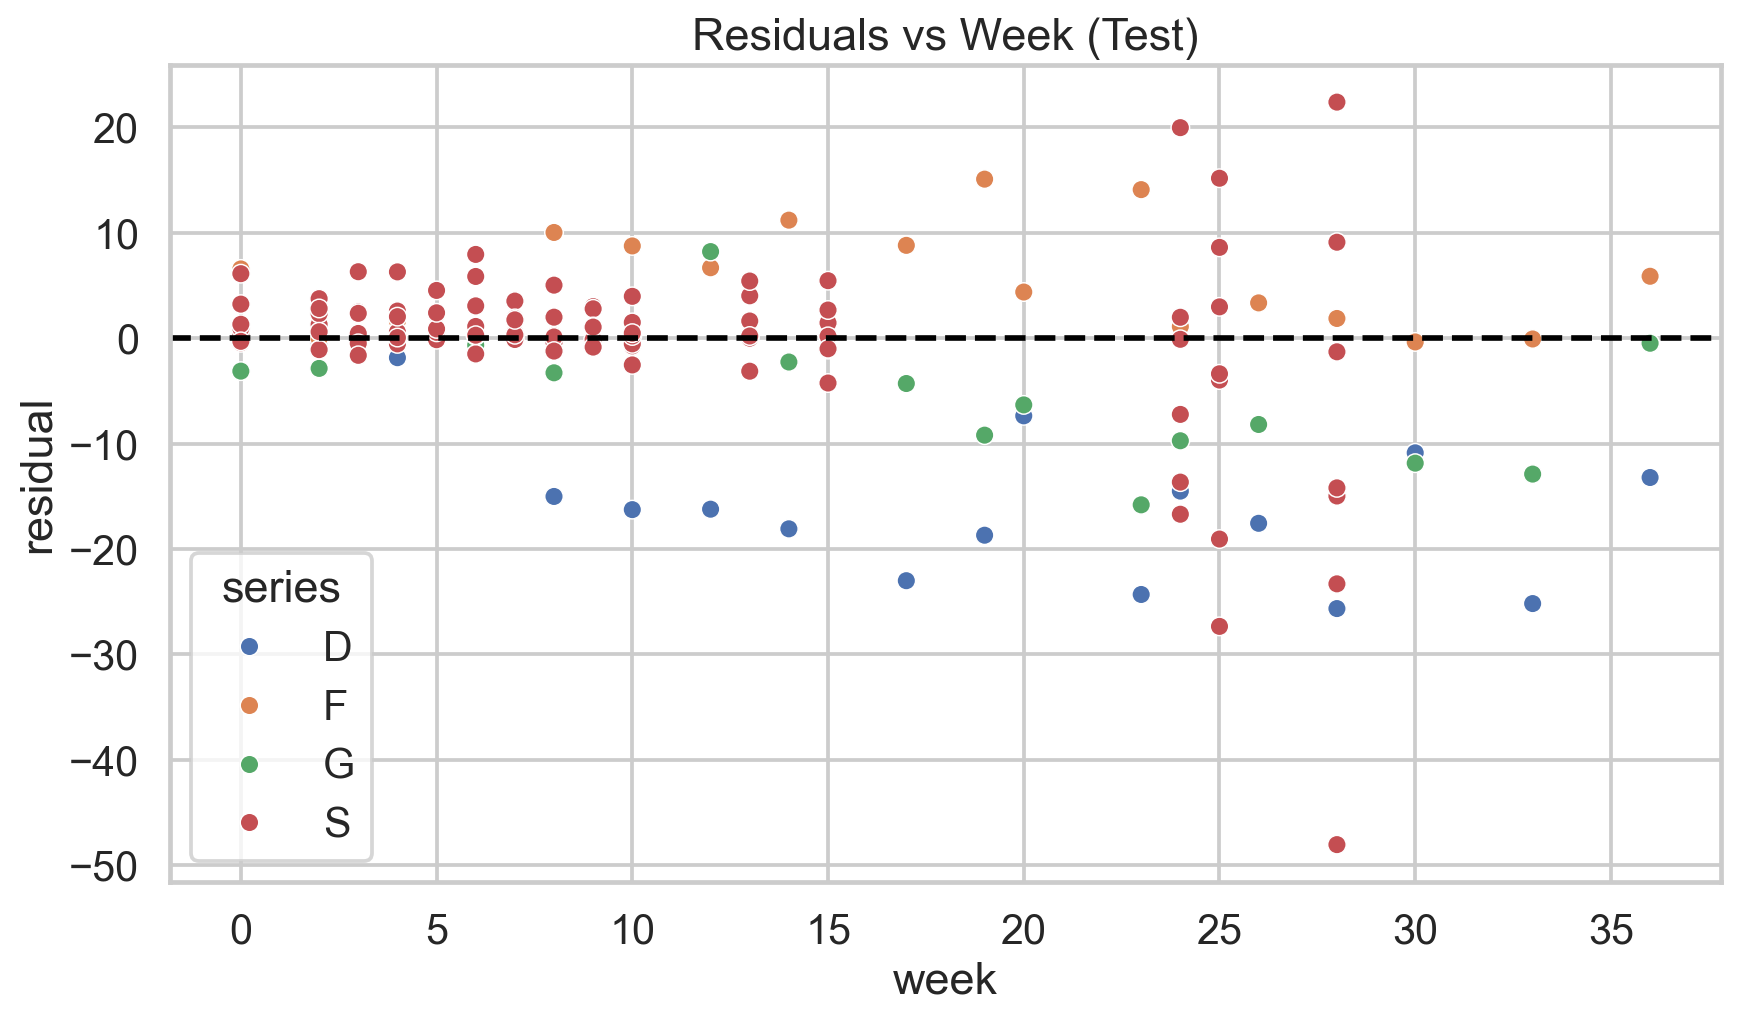
\includegraphics[width=0.75\textwidth]{fig_4_2_main2_residual_vs_week.png}
\caption{Deep-embedding phase, image-only model: residuals (predicted minus
observed peak rust percentage) on the held-out test partition, by
observation week and specimen series. Residuals drift increasingly negative
at later weeks, indicating systematic underestimation of severe, late-stage
corrosion. Reproduced from the phase's own saved diagnostic figure.}
\label{fig:phase2-residuals}
\end{figure}

These findings support a narrower conclusion than either "deep embeddings
work" or "deep embeddings failed." A frozen deep representation was feasible
for current-week visible-corrosion estimation, reaching accuracy broadly
comparable to the handcrafted-feature baseline. Adding metadata to that
representation did not yield a stable improvement in this saved experiment:
it helped during training but not on the final held-out partition, and the
comparison was not confirmed independently of the selection step. The
representation also offered materially less interpretability than the
explicit handcrafted descriptors of the previous phase — a 512-dimensional
embedding does not, by inspection, reveal which visual cues drive a
prediction the way a rust-percentage threshold does. Combined with the
late-stage underestimation problem and the absence of any progress on
structural or remaining-service-life questions, these results motivated a
return to explicit, interpretable image descriptors, alongside a shift
toward posing more demanding questions about hidden structural condition
rather than continuing to refine current-corrosion estimation alone.

\section{Interpretable Corrosion Quantification and Structural-Condition Feasibility}
\label{sec:phase3}

The fourth phase is the project's largest single body of work in this
period and marks a scientific turning point. It replaced the deep embedding
with a broad, explicitly engineered feature representation — ninety-one
descriptors spanning corrosion amount, spatial distribution along the
specimen, surface morphology, colour in three colour spaces (RGB, HSV, and
Lab), and texture — computed by a Python image-processing pipeline. This
pipeline was inspired by the predecessor thesis's manual image-analysis
workflow but is best described as a Python reconstruction and extension of
that workflow's ideas rather than an exact reproduction of it: the original
workflow combined manual GIMP/BIMP editing steps with a separate MATLAB
analysis stage, whereas this phase implements comparable descriptors
programmatically, in some cases extending beyond what the manual workflow
computed.

This phase was also the first to pose two further questions
beyond current-corrosion estimation: whether visible corrosion could help
estimate a specimen's hidden structural condition, and whether a
degradation trajectory and threshold-crossing screening quantity could be
derived from the resulting estimates. Both required confronting the
asymmetry between dense visible-corrosion supervision and sparse structural
supervision established in Section~\ref{sec:structural-supervision}, and
both were evaluated under all three of the grouped evaluation regimes
defined in Section~\ref{sec:eval-regimes} — the first phase in the project
to do so systematically.

\subsection{Visible-corrosion modelling}
\label{sec:phase3-corrosion}

For the two continuous visible-corrosion targets, several candidate model
families were compared (linear regression, RandomForest, histogram-based
gradient boosting, and a small multilayer perceptron); the specific
family selected as best differs by target and by evaluation regime, and is
not repeated model-by-model here. Two categorical severity targets were
also modelled, using the historical \emph{five}-category ordinal scheme in
place at this phase's dataset snapshot (Section~\ref{sec:dataset-audit}) —
these results must not be described as four-class classification, which
belongs to the later, separate dataset and classification effort
(Section~\ref{sec:representation}, strategy~E).

Table~\ref{tab:phase3-results} reports the best mean result for each target
under each evaluation regime. Under a grouped specimen holdout, both
continuous targets are estimated with useful accuracy (total rust: MAE 1.38,
$R^2=0.646$; peak rust: MAE 4.21, $R^2=0.784$). Robustness to campaign
holdout is reasonable — accuracy declines but both targets retain positive
$R^2$ under leave-one-campaign-out. Robustness to treatment holdout is
markedly weaker: mean $R^2$ across treatment folds becomes negative for both
targets, reflecting that individual treatment groups are small
(Section~\ref{sec:loto}) and that at least one held-out treatment fold
produces a strongly negative per-fold $R^2$, pulling the average down. The
five-category classification targets follow a similar pattern: grouped
holdout accuracy is moderate to good (0.83 for total-rust category, though
macro-F1 of 0.573 reveals the imbalance-sensitive weakness that accuracy
alone would hide), and macro-F1 does not exceed roughly 0.47 under either
stricter regime. Read together, visible-corrosion estimation is the most
robustly image-driven layer of this phase: it degrades under distribution
shift, as expected of any model facing genuinely new treatment or campaign
conditions, but it does not collapse.

\subsection{Structural-condition feasibility}
\label{sec:phase3-structural}

The structural-condition models require more careful description, because
several aspects of their design materially affect what the results can be
taken to show. As established in Section~\ref{sec:structural-supervision},
only 48 rows in the dataset carry a structural label, one per specimen.
The feature set used to predict these targets is not image-only: it
combines specimen/exposure metadata, the \emph{manually assigned} visible-corrosion
labels and their categories (the ground-truth annotations, not the previous
subsection's model predictions of them), and a subset of the engineered
image descriptors. The pipeline's own predicted corrosion values are not
included in this feature list, so the damage stage does not chain a learned
corrosion prediction into a learned damage prediction; it instead poses a
single, direct estimation problem — from metadata, manual labels, and image
descriptors together to structural condition — rather than a
strictly image-based inference.

Under a grouped specimen holdout, both structural targets show a modest but
non-trivial relationship to the available features: wire-area loss reaches
MAE 3.90 ($R^2=0.310$), and ultimate load reaches MAE 0.121~kN
($R^2=0.385$) on this phase's own 38/10 grouped-holdout split. These are
this phase's own historical results, computed on its own 792-row dataset
basis and its own feature engineering, and are not compared numerically
against the later terminal-load-focused results discussed in a subsequent
section, which use a different pipeline, feature set, and dataset
alignment.

Under either stricter evaluation regime, performance deteriorates
substantially. Leave-one-campaign-out mean $R^2$ becomes negative for both
targets ($-0.39$ for wire-area loss, $-8.36$ for ultimate load), and
leave-one-treatment-out is similarly negative and, for ultimate load, more
severely so ($-4.57$). Figure~\ref{fig:phase3-robustness} places these
alongside the visible-corrosion results from the previous subsection: the
contrast between the two rows of bars is the central diagnostic finding of
this phase. The available evidence does not support reliable image-based
recovery of hidden structural condition under either stricter regime tested
here. The visible-corrosion layer is markedly more robust overall — both of
its targets retain positive $R^2$ under leave-one-campaign-out — but it is
not uniformly robust: leave-one-treatment-out is less stable and drives
both visible-corrosion targets to negative mean $R^2$ as well
(Table~\ref{tab:phase3-results}), so the two stricter regimes should not be
treated as interchangeable when comparing the two target families.

\begin{table}[htbp]
\centering
\caption{Representative results by target and evaluation regime, interpretable
multi-family feature phase. Model shown is the best-mean-MAE candidate for
that (target, regime) cell. Rust and wire-area-loss targets are in percent;
ultimate load is in kN. All results computed on this phase's own
792-row dataset basis; see Section~\ref{sec:dataset-audit} for how this
differs from the later canonical basis.}
\label{tab:phase3-results}
\begin{tabular}{p{3.6cm}p{2.5cm}p{1.5cm}p{1.2cm}p{1.3cm}}
\toprule
Target & Regime & Model & MAE & $R^2$ \\
\midrule
Total rust (visible) & Grouped holdout & RF & 1.38 & 0.646 \\
Total rust (visible) & LOTO & MLP & 1.53 & $-0.677$ \\
Total rust (visible) & LOCO & RF & 2.10 & 0.582 \\
\midrule
Peak rust (visible) & Grouped holdout & MLP & 4.21 & 0.784 \\
Peak rust (visible) & LOTO & RF & 4.74 & $-0.077$ \\
Peak rust (visible) & LOCO & HGB & 6.21 & 0.595 \\
\midrule
Wire-area loss (structural) & Grouped holdout & RF & 3.90 & 0.310 \\
Wire-area loss (structural) & LOTO & HGB & 10.76 & $-5.481$ \\
Wire-area loss (structural) & LOCO & HGB & 12.28 & $-0.387$ \\
\midrule
Ultimate load (structural) & Grouped holdout & RF & 0.121 & 0.385 \\
Ultimate load (structural) & LOTO & RF & 0.158 & $-4.569$ \\
Ultimate load (structural) & LOCO & ExtraTrees & 0.624 & $-8.356$ \\
\bottomrule
\end{tabular}
\end{table}

\begin{figure}[htbp]
\centering
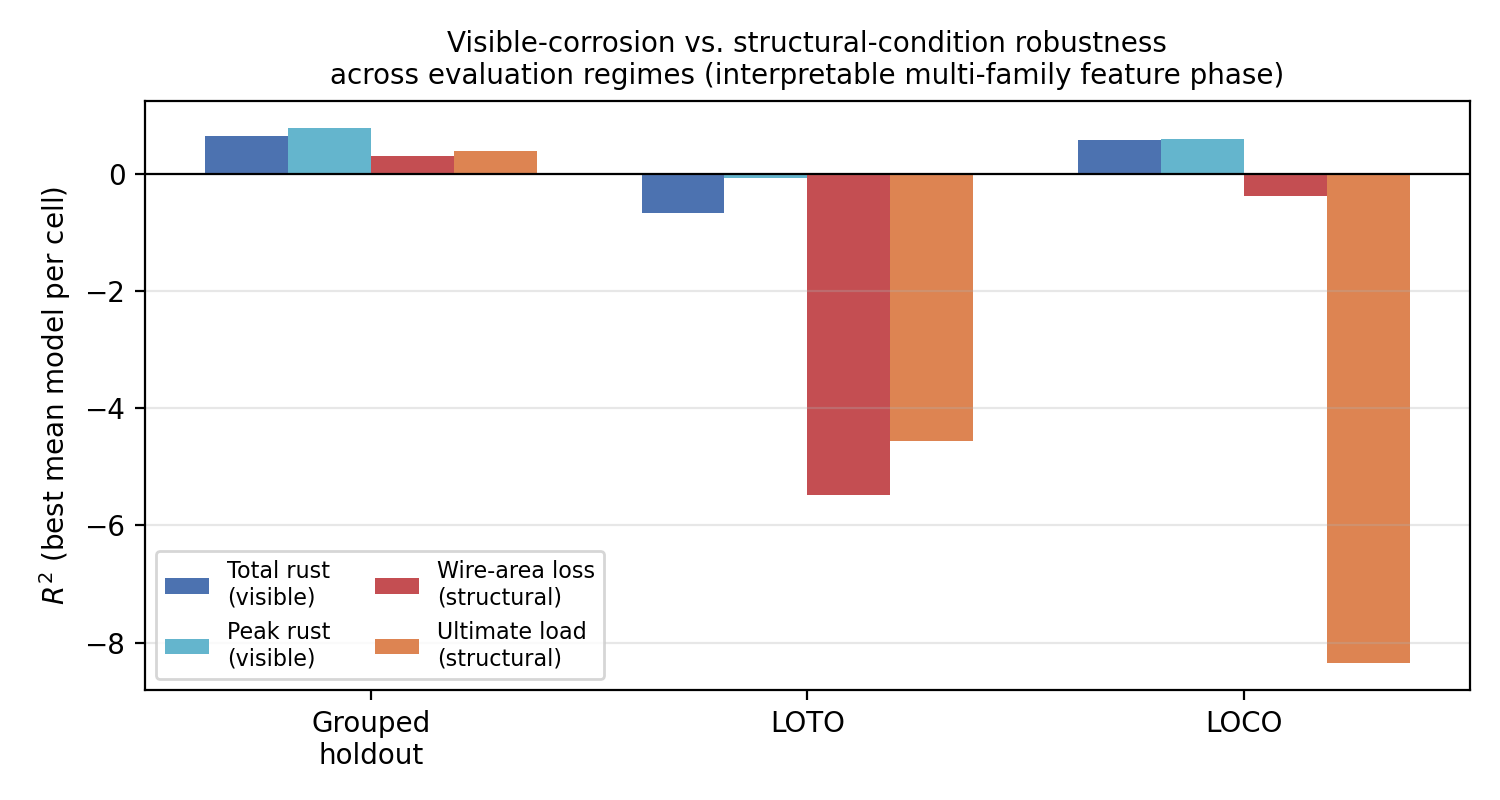
\includegraphics[width=0.85\textwidth]{fig_4_3_main3_robustness_by_regime.png}
\caption{Best-mean-model $R^2$ by evaluation regime for the two
visible-corrosion targets and the two structural-condition targets,
interpretable multi-family feature phase. Visible-corrosion models are
substantially more robust than the structural models overall, and both
visible-corrosion targets retain positive $R^2$ under leave-one-campaign-out;
leave-one-treatment-out is less stable and produces negative mean $R^2$ for
both visible-corrosion targets as well, while the structural targets
deteriorate far more severely under both stricter regimes. Generated
directly from the phase's own saved regression-metrics tables
(Table~\ref{tab:phase3-results}).}
\label{fig:phase3-robustness}
\end{figure}

Three further diagnostics, reported directly in this phase's own technical
report, explain why. First, correlation between the manually labelled
visible-corrosion measures and wire-area loss is close to zero across the
48 structural rows (total rust: $r=0.021$; peak rust: $r=0.011$) — visible
corrosion, as measured here, is only weakly related to internal wire loss
even before any modelling is attempted. Second, feature-importance analysis
of the full-data ultimate-load model shows its largest contributions coming
from steel-mesh count and campaign indicator variables, not from image
descriptors — the same campaign-linked metadata dominance later quantified
more thoroughly in Section~\ref{sec:confounding}'s discussion of design
confounding. Third, the "final" structural estimator for each target is fit
on all 48 structural rows with no further held-out partition at that step,
and is then applied to every observation in the dataset — including
non-terminal weeks — to produce an estimated structural condition at each
week. These estimates are the model-derived quantities introduced in
Table~\ref{tab:quantity-availability}: they are the output of a model fit
in-sample on the full structural subset, not a repeated physical
measurement, and the degradation curves built from them in later work
inherit this property.

\subsection{What this phase established}
\label{sec:phase3-synthesis}

This phase's evidence supports several specific conclusions, stated here
without extrapolation beyond what was tested. Interpretable image
descriptors can estimate visible corrosion with useful accuracy, including
under a meaningful campaign-holdout stress test. Visible-corrosion
estimation is considerably better supported by the available evidence than
hidden structural-condition estimation. Structural inference in this
dataset is constrained by the combination of sparse supervision (48 rows,
one per specimen), small and unevenly sized treatment groups, and
campaign-linked design variables that dominate the structural models'
feature importances. The structural-condition stage is a mixed-input
estimation problem — metadata, manual corrosion labels, and image
descriptors together — not an image-only inference.

It is also this phase's own technical report, not a subsequent phase, that
first names campaign confounding and the risk of a "downstream label
shortcut" (structural models drawing signal from manually assigned
corrosion labels and design metadata rather than from independently
learned image content) as explicit concerns. Work described in later
sections that quantifies these problems more rigorously and responds to
them with dedicated diagnostics and a reframed research question should
therefore be understood as acting on a problem this phase had already
identified, not as discovering it for the first time.

That reframing followed directly from the findings above. The sparse,
campaign-confounded structural signal recovered here motivated stronger
attention to out-of-sample structural estimation, explicit
image-versus-metadata ablations, robustness-oriented model selection,
feature cleanup, and monotonicity-aware degradation modelling, and
ultimately a reconsidered structural research question targeting one of
the two directly measured terminal endpoints available in the dataset.

\section{Degradation Modelling and Proxy-RUL Feasibility}
\label{sec:phase3-degradation}

The same phase also carried out a feasibility experiment in the derived
screening quantity introduced in Section~\ref{sec:proxy-rul}: for each of the
48 specimens, a degradation curve was fitted to each of four per-week
series — the two directly observed visible-corrosion measures and the two
model-estimated structural measures from Section~\ref{sec:phase3-structural}
— and projected forward to identify when it would cross an engineering
threshold. This section reports what that experiment actually produced, and
is deliberately brief: the exercise is a feasibility check on the
derivation chain itself, not a second opportunity to validate structural
prediction.

Curve fitting used piecewise-linear and exponential families, selected per
specimen and target. Fit quality was good for the two visible-corrosion
series (median $R^2$ of 0.90 and 0.92) and moderate for the two
model-estimated structural series (median $R^2$ of 0.64 and 0.60) — every
curve was fit to the same 15–18 observation weeks per specimen established
in Section~\ref{sec:longitudinal}, so the structural curves are trajectories
through model-estimated values, not through repeated physical
measurements. The final proxy-RUL for a specimen was defined as the
earliest of three threshold-crossing events read off these curves and
projected up to 104 weeks beyond the last observation: a 25\% wire-area-loss
crossing, an ultimate-load crossing at 80\% of a campaign reference load, or
a crossing of a composite health index combining all four series.

Of the 48 specimens, 33 received a finite proxy-RUL estimate within the
104-week projection horizon; the remaining 15 never crossed any threshold
within that horizon and are right-censored. Of the 33 finite estimates,
23 — the large majority — are exactly zero weeks, meaning the relevant
threshold was already crossed at the specimen's last available observation
rather than projected into the future. Figure~\ref{fig:phase3-rul-histogram}
shows this concentration directly. Only the remaining ten specimens carry a
proxy-RUL that is both finite and genuinely forward-looking, ranging up to
55.5 weeks.

\begin{figure}[htbp]
\centering
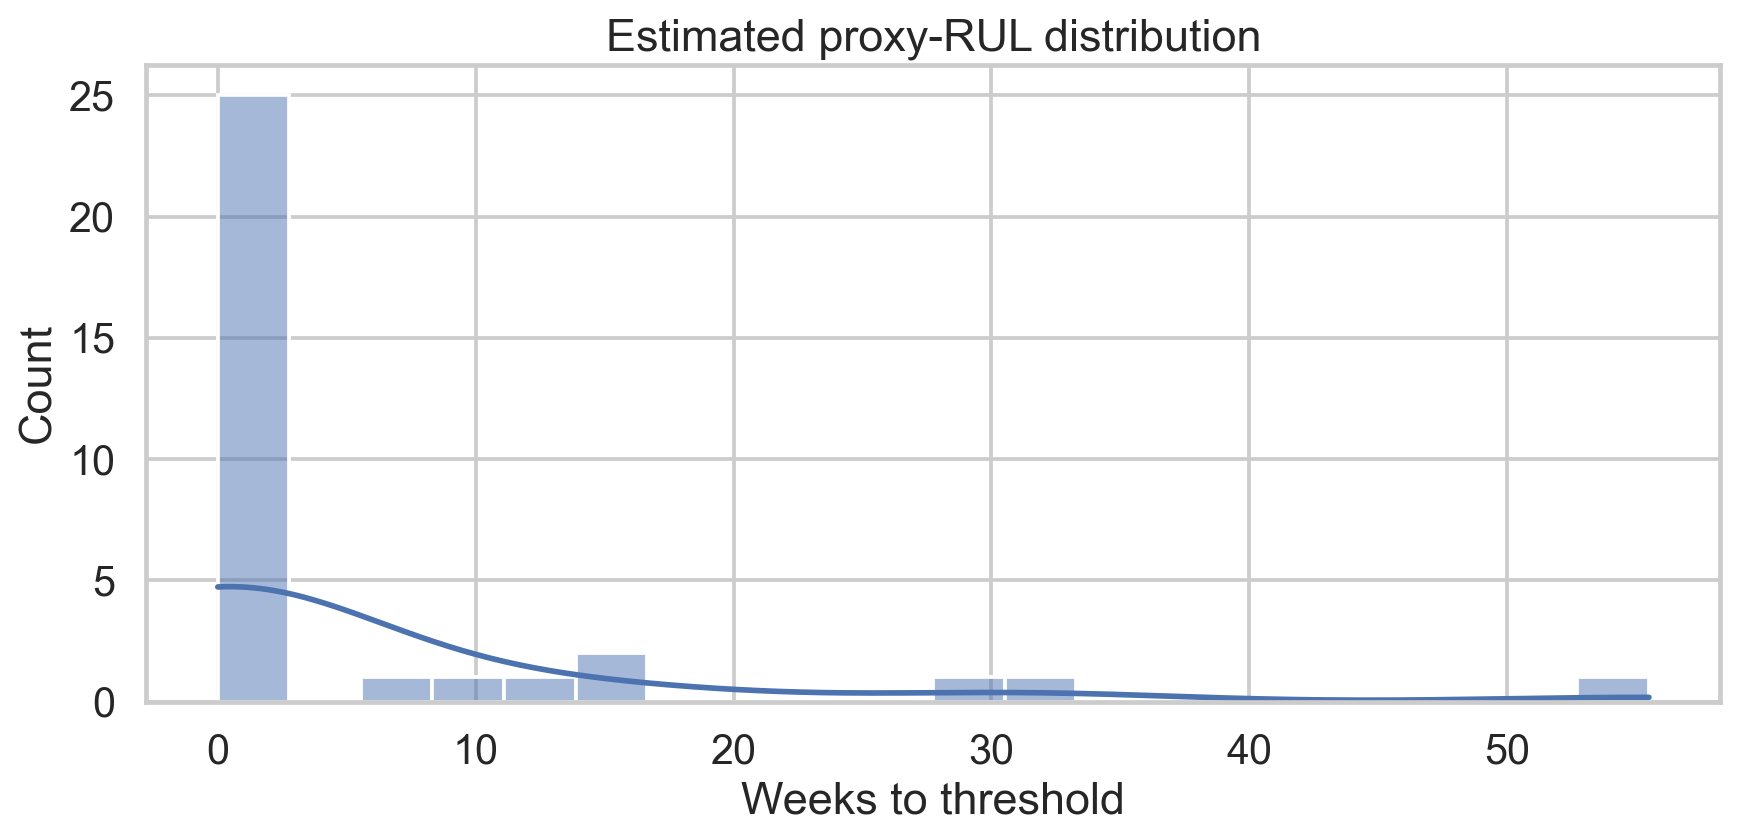
\includegraphics[width=0.72\textwidth]{fig_4_4_main3_proxy_rul_histogram.png}
\caption{Distribution of finite proxy-RUL estimates (33 of 48 specimens);
the remaining 15 specimens are right-censored (no threshold crossing within
the 104-week projection horizon) and are not shown on this axis. Most
finite estimates are at or near zero weeks. Reproduced from the phase's own
saved output.}
\label{fig:phase3-rul-histogram}
\end{figure}

This outcome illustrates, concretely, why the quantity is a feasibility
result rather than a validated remaining-service-life estimate. Every stage
of the derivation compounds the uncertainty of the stage before it: the
structural curves are fitted to estimates that are themselves weak under
distribution shift (Section~\ref{sec:phase3-structural}), the curve family
and threshold are modelling choices rather than physical constants
(Section~\ref{sec:proxy-rul}), and the 104-week extrapolation horizon
extends well beyond any observed data for most specimens. The pipeline is a
working demonstration that the four-step derivation from repeated observed
and model-estimated condition series to a threshold-crossing screening
quantity can be executed end to end; it does not, and was not designed to,
constitute evidence that the resulting numbers are accurate estimates of
true remaining service life.

\section{Robustness and Diagnostic Refinement}
\label{sec:phase4a}

The next phase of work continued directly from the structural-condition
findings above, using the same underlying dataset structure but a more
rigorous implementation. This phase's contribution should be stated
precisely: campaign confounding, sparse structural
supervision, and the risk of models drawing on manually assigned labels
rather than independently learned image content were all already named, in
those terms, by the previous phase's own report. This phase's contribution
was to quantify how severe these problems were under systematic testing,
audit the feature set for redundancy, and revise the modelling and
selection procedure in response — acting on a diagnosis the project had
already made, not making it for the first time.

A feature-redundancy audit identified thirteen near-constant columns, one
exact duplicate pair, and thirty-six feature pairs with rank correlation of
0.95 or higher within the engineered feature set — including a pairing
already anticipated in Section~\ref{sec:phase3-corrosion}, since one image
descriptor and the total-rust label are correlated at $\rho=0.9996$, a
near-tautological relationship. More informative for the structural
question is where genuine, non-redundant signal was found: the strongest
univariate correlate of wire-area loss is a single image morphology
feature, but only at $r=0.38$; for ultimate load, the five strongest
univariate correlates are not image features at all, but five metadata and
temporal variables — steel-mesh count, chloride concentration, ageing days,
observation week, and terminal week — each correlated with ultimate load at
exactly the same magnitude, $|r|=0.827$, a direct numerical signature of
the fact that these variables are perfectly aligned with campaign identity
on the 48-row structural subset (Section~\ref{sec:confounding}). This
answers, for the ultimate-load target specifically, where the apparently
predictive structural signal actually originates: from experimental design
metadata that happens to be campaign-linked, not from the corrosion images.

The phase's own robustness benchmark, summarised in
Table~\ref{tab:phase4a-robustness} and Figure~\ref{fig:phase4a-collapse},
quantifies the consequence for the two target families side by side —
deliberately, because the two families behave very differently and must
not be described with a single verdict. Visible-corrosion targets remain
stable or even improve in relative terms under leave-one-campaign-out
(surface total rust: 0.77$\times$ its own grouped-holdout MAE; peak rust:
0.96$\times$), with Spearman correlation staying above 0.97 in both cases.
Structural targets do not: ultimate load's leave-one-campaign-out MAE is
3.24 times its grouped-holdout value, with Spearman falling to 0.35, and
wire-area loss's leave-one-campaign-out Spearman turns negative
($-0.089$). The robustness collapse documented here belongs to the
structural stage; it is not a property of the pipeline as a whole, and the
visible-corrosion layer's continued robustness is as much a part of this
phase's evidence as the structural collapse is.

\begin{table}[htbp]
\centering
\caption{Grouped-holdout and leave-one-campaign-out MAE and Spearman
correlation for the best-performing model per target under each individual
evaluation strategy considered on its own, robustness-quantification phase.
This is a per-strategy diagnostic comparison, not necessarily the phase's
final robustness-weighted model selection (see following paragraph). Rust
targets in percent, wire-area loss as a fraction, ultimate load in kN.
Source: the phase's own saved robustness-benchmark table.}
\label{tab:phase4a-robustness}
\begin{tabular}{p{4.0cm}p{2.4cm}p{1.2cm}p{1.2cm}p{1.4cm}}
\toprule
Target & Regime & Model & MAE & Spearman \\
\midrule
Surface total rust (visible) & Grouped holdout & GB & 0.177 & 0.999 \\
Surface total rust (visible) & LOCO & GB & 0.136 & 0.997 \\
\midrule
Peak rust (visible) & Grouped holdout & RF & 1.097 & 0.992 \\
Peak rust (visible) & LOCO & RF & 1.058 & 0.977 \\
\midrule
Wire-area-loss fraction (structural) & Grouped holdout & RF & 0.105 & 0.280 \\
Wire-area-loss fraction (structural) & LOCO & RF & 0.124 & $-0.089$ \\
\midrule
Ultimate load, kN (structural) & Grouped holdout & RF & 0.174 & 0.778 \\
Ultimate load, kN (structural) & LOCO & RF & 0.564 & 0.353 \\
\bottomrule
\end{tabular}
\end{table}

\begin{figure}[htbp]
\centering
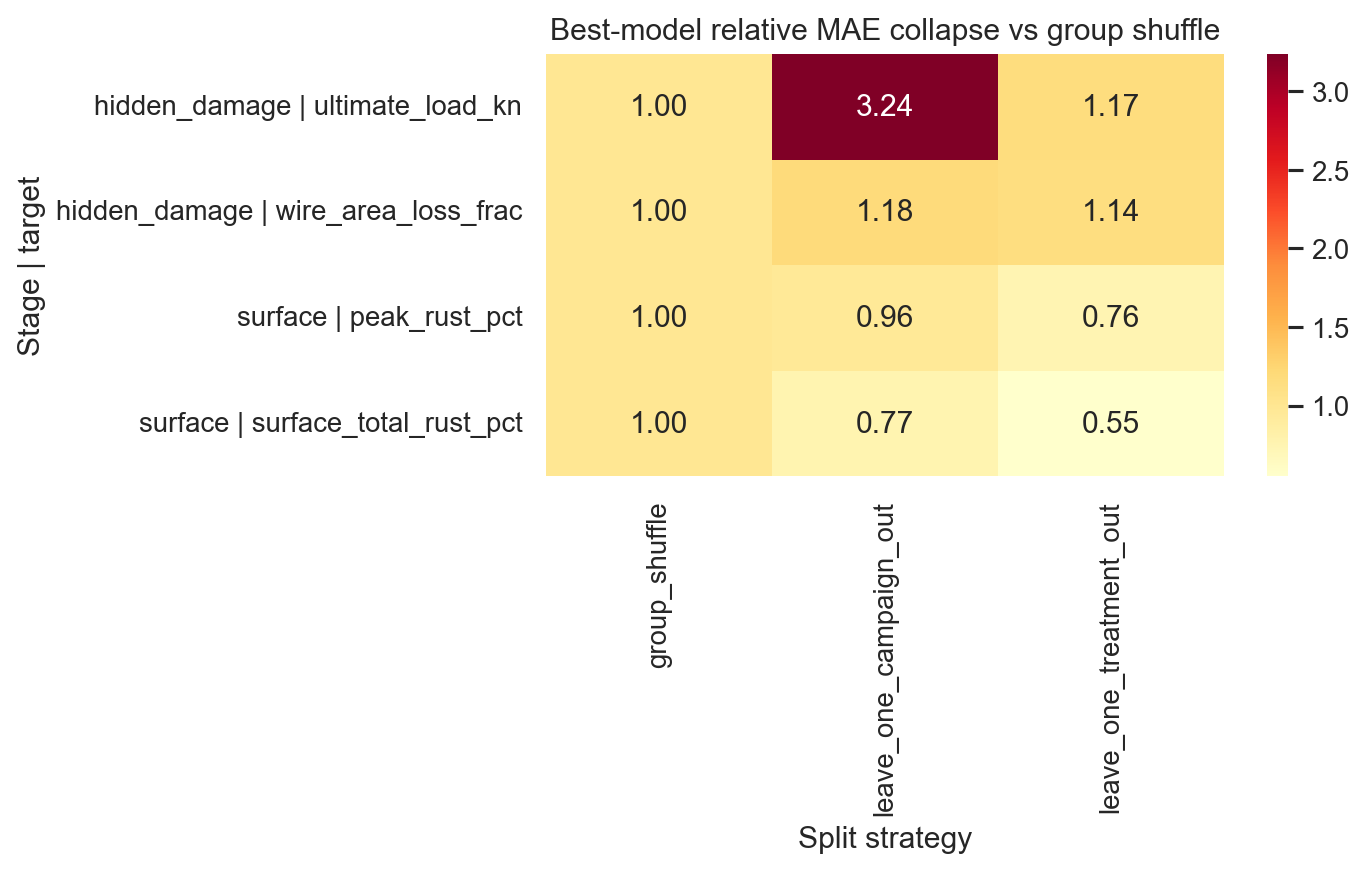
\includegraphics[width=0.75\textwidth]{fig_4_5_main4_relative_mae_collapse_heatmap.png}
\caption{Best-model MAE under each evaluation regime, relative to that
target's own grouped-holdout MAE (1.00 by definition). Visible-corrosion
targets (bottom two rows) stay at or below 1.2$\times$ under every regime;
structural targets (top two rows) inflate sharply under leave-one-campaign-out,
most severely for ultimate load (3.24$\times$). Reproduced from the phase's
own saved diagnostic output.}
\label{fig:phase4a-collapse}
\end{figure}

Table~\ref{tab:phase4a-robustness} should be read as a diagnostic
comparison, not as a statement of which model the phase ultimately
selected: it reports, independently for each target, whichever model
performed best under a given evaluation strategy considered on its own.
The phase's final structural-model selection instead uses the
robustness-weighted procedure described below and is recorded separately
in its own saved best-model table. For ultimate load the two coincide:
RandomForest on the metadata-only feature set is both the per-strategy
diagnostic winner shown above and the phase's final robustness-weighted
selection, with identical metrics. For wire-area-loss fraction they differ:
the per-strategy diagnostic winner in Table~\ref{tab:phase4a-robustness} is
RandomForest, but the phase's final robustness-weighted selection is
CatBoost on the metadata-only feature set (grouped-holdout MAE 0.124,
leave-one-treatment-out MAE 0.116, leave-one-campaign-out MAE 0.121,
grouped-holdout Spearman 0.289) — numerically close to, but not identical
with, the diagnostic table's figures for that target. Both comparisons
agree on the point that matters for this section: regardless of which
specific model is chosen, the structural targets' feature importances and
robustness pattern remain metadata-dominant, in contrast to the
visible-corrosion targets.

Two further changes distinguish this phase's methodology from the previous
one. Structural-target model selection moved from picking whichever model
happened to have the best mean score on a single split, to a weighted
combination emphasising leave-one-campaign-out performance most heavily —
a deliberate response to the previous phase's own observation that
grouped-holdout performance alone was an unreliable guide to structural
robustness. Degradation-curve fitting was also revised: the previous
phase's fits were dominated by a flexible, non-parametric curve family
selected for 44 of 48 specimens, which the project's own review noted can
reach near-zero fitting error by interpolation rather than by capturing a
genuine trend; the revised fitting is more evenly split between that family
and a simpler linear one (21 versus 27 specimens), and degradation status
is now reported as an explicit crossed/not-yet-crossed/censored category
breakdown rather than a single ambiguous "weeks remaining" figure. The
phase's own stated conclusion, after these revisions, is worth reporting
directly: the improved structural models remain metadata-dominant, and the
project does not consider this sufficient support for a claim that surface
image features robustly infer hidden structural damage.

\section{Refocused Terminal Ultimate-Load Study}
\label{sec:phase4b}

The robustness findings above motivated a deliberate change in research
question, not merely a further modelling attempt. Rather than continuing to
target a sparse, model-derived, campaign-confounded hidden-damage estimate,
this phase targets one of the two structural quantities in the dataset
that are directly measured at a single, well-defined terminal time point:
ultimate load, selected here in preference to the other (wire-area loss)
for this refocused analysis. The question posed is correspondingly
specific: after controlling for
specimen design and exposure characteristics, does superficial visible
corrosion provide predictive information about terminal ultimate load
beyond what those design characteristics already carry? Because this
question is about incremental value, not standalone accuracy, every
analysis in this phase compares matched feature-set configurations under
the same model-selection and evaluation procedure, rather than reporting a
single "best" pipeline in isolation.

\subsection{Does corrosion add value over metadata, pooled?}

Table~\ref{tab:phase4b-featuresets} reports the pooled, grouped
cross-validation comparison across seven feature-set configurations, all 48
specimens, ten repeated grouped splits. A metadata-only Ridge regression —
eleven features describing specimen design and exposure, no image content
at all — achieves the lowest mean absolute error (0.173~kN) and the
second-highest Spearman correlation (0.758) of any configuration tested.
Adding HSV colour descriptors to the metadata leaves MAE essentially
unchanged (0.173~kN) while marginally improving Spearman (0.771); adding
RGB descriptors instead makes both metrics worse (MAE 0.184~kN, $R^2=0.584$
versus metadata-only's 0.645). Image descriptors used alone, without
metadata, are clearly the weakest configurations tested (RGB-only MAE
0.253~kN, $R^2=0.269$). Read together, the pooled evidence does not show
image descriptors adding meaningful value over metadata alone, and in one
configuration (RGB) adding them measurably hurts performance.

\begin{table}[htbp]
\centering
\caption{Pooled feature-set comparison, terminal ultimate load, grouped
cross-validation (48 specimens, 10 splits). Model shown is the winning
model for that feature set. Source: the phase's own saved comparison
table.}
\label{tab:phase4b-featuresets}
\begin{tabular}{p{4.1cm}p{1.3cm}p{1.4cm}p{1.1cm}p{1.1cm}p{1.3cm}}
\toprule
Feature set & Features & Model & MAE & $R^2$ & Spearman \\
\midrule
Metadata only & 11 & Ridge & 0.173 & 0.645 & 0.758 \\
Metadata + HSV & 47 & Ridge & 0.173 & 0.635 & 0.771 \\
Metadata + RGB + HSV & 88 & CatBoost & 0.183 & 0.607 & 0.753 \\
Metadata + RGB & 52 & Ridge & 0.184 & 0.584 & 0.748 \\
HSV only & 36 & CatBoost & 0.210 & 0.481 & 0.705 \\
RGB + HSV & 77 & CatBoost & 0.234 & 0.411 & 0.668 \\
RGB only & 41 & CatBoost & 0.253 & 0.269 & 0.501 \\
\bottomrule
\end{tabular}
\end{table}

A subset analysis restricted to the 43 specimens whose terminal corrosion
was above a near-zero onset threshold shows a modest, narrower reversal:
there, the combined metadata-plus-RGB-plus-HSV configuration edges ahead of
metadata-only on MAE (0.163 vs.\ 0.173~kN) and $R^2$ (0.660 vs.\ 0.633),
although metadata-only retains a marginally higher Spearman correlation
(0.803 vs.\ 0.791) even in this subset. This is reported as a narrow,
subset-specific observation consistent with image descriptors being more
competitive once a specimen has developed measurable corrosion, not as a
reversal of the pooled conclusion above.

\subsection{What happens within a single mesh family?}

The specimen design matrix in Section~\ref{sec:experimental-context} means
that campaign identity, steel-mesh count, and chloride level co-vary almost
perfectly. Table~\ref{tab:phase4b-featuresets} is therefore a pooled result
across two structurally different specimen designs, and the phase's own
analysis goes on to ask what the same comparison shows within each
mesh family alone. The answer is an important caution against reading the
pooled MAE values too optimistically: within either the 4-mesh or the
7-mesh group individually (24 specimens each), every feature-set
configuration achieves a \emph{negative} mean $R^2$ (4-mesh: $-0.81$ to
$-3.56$; 7-mesh: $-0.30$ to $-4.65$), even for the configurations whose raw
MAE looks numerically similar to the pooled result (0.14–0.26~kN). A
negative $R^2$ means the model performs worse than simply predicting the
group mean for every specimen. Rank correlation is correspondingly weak
(the best Spearman achieved within 4-mesh is only 0.10; within 7-mesh,
0.46). A low mean-absolute-error number within a small, low-variance
subgroup is not, by itself, evidence of a working predictive relationship,
and this dataset provides a direct illustration of that gap between
absolute error and explained variance.

\subsection{Is the pooled corrosion-load correlation genuine?}

The clearest illustration of the same point uses correlation directly
rather than a fitted model. Pooled across both mesh families, terminal
visible corrosion and terminal ultimate load are correlated at Spearman
$\rho=0.462$ ($p=0.0009$, $n=48$) — a relationship that would ordinarily be
read as a moderate, statistically significant positive association.
Stratified by mesh family, this relationship does not merely weaken: within
the 4-mesh group it is statistically indistinguishable from zero
($\rho=-0.046$, $p=0.83$), and within the 7-mesh group it is negative and
borderline significant in the \emph{opposite} direction ($\rho=-0.401$,
$p=0.052$). Figure~\ref{fig:phase4b-mesh-scatter} shows all three panels
together; the phase's own saved output table labels the pooled figure
explicitly as a "confounded" reference for this reason. This pattern is
evidence of substantial confounding by mesh/campaign group structure — the
pooled trend is strongly influenced by between-group differences (the
lower-mesh, higher-load group also happens to have lower corrosion), rather
than demonstrating a direct effect of corrosion on load-bearing capacity.
It does not, on its own, prove that no corrosion-capacity relationship
could exist under other conditions, nor does it fully decompose the pooled
association into its causal components; it shows only that the pooled
correlation in this dataset cannot be used as evidence for one.

\begin{figure}[htbp]
\centering
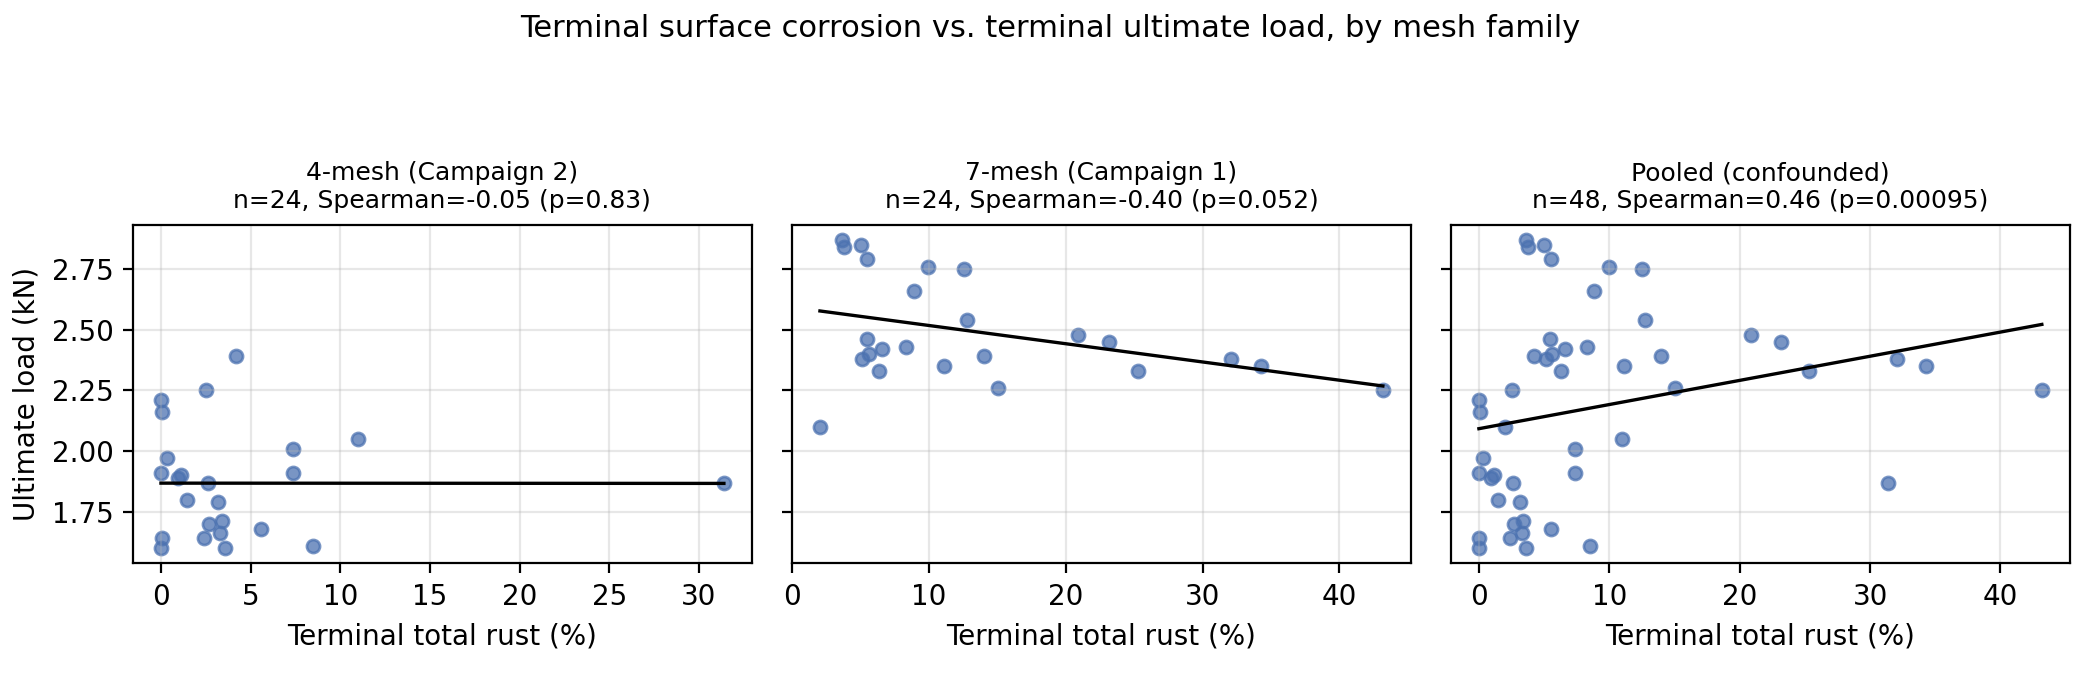
\includegraphics[width=0.95\textwidth]{fig_4_6_mesh_stratified_corrosion_vs_load.png}
\caption{Terminal surface total rust percentage versus terminal ultimate
load, stratified by steel-mesh family and pooled. The positive pooled
association is not reproduced within either mesh family: it is
approximately null in the 4-mesh group ($\rho\approx-0.05$) and negative in
the 7-mesh group ($\rho\approx-0.40$). Generated directly from the phase's
own saved specimen-summary table.}
\label{fig:phase4b-mesh-scatter}
\end{figure}

\subsection{Robustness under campaign holdout, and a residual-correction attempt}

Under leave-one-campaign-out — the most demanding regime available, and,
per Section~\ref{sec:confounding}, a test of extrapolation across the mesh
and chloride design space rather than ordinary generalisation — every
feature-set configuration collapses to strongly negative $R^2$ (metadata-only:
MAE 0.465~kN, $R^2=-4.64$). This is consistent with, rather than
contradicting, the pooled-versus-stratified finding above: a model trained
entirely within one mesh/campaign design space has no basis for
extrapolating to a design space it has never seen, regardless of which
features it was given. A further attempt to recover some of this
performance by adding a second-stage, mesh-aware residual correction on top
of the metadata-only baseline was tested and \emph{worsened} MAE, RMSE, and
Spearman relative to the baseline alone — a negative result the phase's own
saved comparison records explicitly rather than omitting.

\subsection{Synthesis}

Taken together, the evidence from this phase supports a specific and
bounded conclusion: for terminal ultimate load, pooled across the observed
specimen designs, specimen and exposure metadata is the strongest available
predictor, and visible corrosion descriptors do not provide a reliable
pooled improvement over it — with a narrow exception in a corrosion-onset
subset that does not overturn the pooled result, and with within-mesh and
cross-campaign evaluation both showing that whatever apparent relationship
exists in the pooled data is confounded by, or fails to extrapolate across,
specimen design. This is a materially more defensible scientific claim than
either "corrosion predicts structural capacity" or "corrosion is
irrelevant to structural capacity" — it is a claim about incremental
predictive value, tested directly, under conditions designed to expose
confounding rather than obscure it.

\section{Four-Class Corrosion Classification and Augmentation}
\label{sec:phase5}

The final activity considered in this chapter is a later and structurally
separate effort, addressing a different task from every phase above: direct
image classification into an ordinal visible-corrosion severity category,
using the raw-image deep-classification strategy introduced in
Section~\ref{sec:representation} (strategy~E). It targets the
\emph{current}, four-level severity schema established in
Section~\ref{sec:dataset-audit} (Table~\ref{tab:category-schema}) — not the
five-level historical schema modelled in
Section~\ref{sec:phase3-corrosion} — and is implemented as a standalone
pipeline with no code dependency on any earlier phase.

The current schema is severely imbalanced: of 791 usable images, 658
(83.2\%) fall in the lowest severity class, against 99, 20, and 14 images
in the three more severe classes respectively (Table~\ref{tab:data-modalities}).
This imbalance directly shaped the data-preparation work carried out so
far. A five-recipe augmentation methodology — spanning brightness/contrast
adjustment, saturation and colour-balance adjustment, blur and noise, a
compound recipe, and a mirror-flip-plus-brightness recipe — was applied to
every one of the 791 original images at a uniform six-fold expansion (one
original plus five augmented copies), producing a \emph{global offline
augmentation inventory} of 4{,}746 images (791 originals plus 3{,}955
augmented copies; Table~\ref{tab:phase5-classdist}). Because the expansion
factor is identical across classes, this inventory preserves the original
class proportions exactly.

Specimens were then assigned to training, validation, and test partitions
at the specimen level, consistent with the grouping principle of
Section~\ref{sec:leakage}, with a leakage-safety rule enforced on top of
that assignment: any augmented copy whose original image belongs to a
validation- or test-assigned specimen is excluded from every split, so
that validation and test contain only original, unaugmented images (75
each) and no augmented copy of a held-out specimen ever reaches the
training set. Because validation and test together account for 150 of the
791 original images, their 750 associated augmented copies ($150\times5$)
are removed from the global inventory before splitting. The resulting
manifests therefore contain 3{,}846 training rows (641 original images plus
3{,}205 of their augmented copies), 75 validation rows, and 75 test
rows — 3{,}996 rows used in total, not the full 4{,}746-image inventory.
The training manifest's own class distribution is 3{,}156/540/78/72
(82.1\%/14.0\%/2.0\%/1.9\%), close to but not identical with the global
inventory's proportions, since which original specimens — and therefore
which of their augmented copies — fall into validation or test is not
itself class-balanced. The majority class remains dominant throughout, and
the project's own documentation identifies class-weighting or an
equivalent technique as a remaining requirement for whichever training
procedure is used next.

\begin{table}[htbp]
\centering
\caption{Global offline augmentation inventory (before leakage-safe
exclusion of held-out specimens' augmented copies), four-class severity
schema. Every class is expanded by the same factor, so relative
proportions within this inventory are unchanged; this table does not
represent the final training-manifest composition (3{,}846 rows; see text).
Source: the effort's own dataset-preparation report.}
\label{tab:phase5-classdist}
\begin{tabular}{ccccc}
\toprule
Class (severity) & Original images & Augmented copies & Total & Factor \\
\midrule
1 (lowest) & 658 & 3{,}290 & 3{,}948 & 6$\times$ \\
2 & 99 & 495 & 594 & 6$\times$ \\
3 & 20 & 100 & 120 & 6$\times$ \\
4 (highest) & 14 & 70 & 84 & 6$\times$ \\
\bottomrule
\end{tabular}
\end{table}

A mirror (horizontal) flip is included among the accepted recipes here,
even though the same transformation is explicitly excluded from the
regression work in earlier phases (Section~\ref{sec:representation}). The
distinction is deliberate and physically grounded rather than
inconsistent: total visible-corrosion severity, the target of this task, is
position-invariant — a mirrored image has the same overall severity — whereas
the strip-position and rust-location descriptors used in the regression
phases encode left-right position on the specimen directly, and a flip
would silently invalidate those features' meaning. Several other
augmentations were considered and rejected on physical-plausibility
grounds: label-blending techniques such as MixUp and CutMix were excluded
because the severity classes are discrete and cannot be meaningfully
interpolated or partially overwritten; synthetic image generation was
excluded as infeasible given fewer than twenty training images in the
smallest classes; and elastic deformation, cutout, large rotation, vertical
flip, and heavy colour shift were all excluded as producing image content
inconsistent with how the specimens were actually photographed. Leakage
safety is enforced by a runtime check in the splitting code, which raises
an error if any augmented image is found in the validation or test
partition, rather than relying on documentation alone.

The status of this effort should be stated plainly. Dataset preparation is
complete: the target schema is defined, the class distribution is
characterised, specimen-level splitting is implemented and verified, and
the augmentation pipeline has been run to produce the expanded training
pool described above. No classifier has been trained, compared, or
evaluated on this data at the time of writing — no ResNet-50 or Vision
Transformer fine-tuning, and no accuracy, macro-F1, or confusion-matrix
result exists for this task in the repository. Data preparation for the
four-class classification task is complete; classifier training and
evaluation remain future work.


% =============================================================
% Chapter 5 -- Integrated Results and Comparative Analysis
% =============================================================
\chapter{Integrated Results and Comparative Analysis}
\label{ch:results}

Chapter~\ref{ch:activities} reconstructed the project chronologically, phase
by phase. This chapter does not repeat that chronology. It instead
integrates the evidence across phases to answer the scientific questions
that recur throughout the project's history: how reliably visible corrosion
and hidden structural condition can each be estimated, what images
contribute once metadata is already available, how conclusions change under
stricter evaluation, what can and cannot be said about degradation and
service life, and what the classification branch currently supports. Facts
already established in Chapters~\ref{ch:dataset}--\ref{ch:activities} are
cited by reference rather than re-derived.

\section{Scope and Rules for Cross-Phase Comparison}
\label{sec:results-scope}

The project's successive phases differ in dataset basis (792 rows with one
imputed observation versus 791 aligned rows, Section~\ref{sec:dataset-audit}),
target definition, feature representation, split construction, number of
folds, model-selection procedure, use of manually assigned labels, and, for
the categorical targets, the number of severity classes
(Table~\ref{tab:category-schema}). A lower MAE or higher $R^2$ in one phase
than another does not, by itself, establish that one phase's approach is
superior: it may instead reflect a different, non-comparable protocol.

This chapter therefore distinguishes three kinds of comparison: a
\emph{direct numerical comparison}, permitted only where target, feature
set, dataset basis, and evaluation regime are sufficiently aligned, with
remaining protocol differences stated alongside the numbers; a \emph{ratio
comparison}, which normalises a result against its own phase's baseline
(e.g.\ a stricter-regime MAE divided by that same model's grouped-holdout
MAE) so only relative degradation, not absolute error, crosses phases; and
a \emph{qualitative comparison} of scientific conclusions, robustness
patterns, and failure modes rather than metric values. Most comparisons
below are of the second or third kind.

\section{Visible-Corrosion Estimation}
\label{sec:results-visible}

\subsection{Current-corrosion estimation}

Across the project, visible surface corrosion is the quantity estimated
with the most consistent success. The classical baseline reached a grouped-
holdout $R^2$ of 0.900 for current-week peak rust
(Section~\ref{sec:phase1}); the interpretable multi-family feature phase
reached $R^2=0.646$ (total rust) and $R^2=0.784$ (peak rust) under the same
regime (Section~\ref{sec:phase3-corrosion}). These results are not placed
on a single ranked list, because they use different feature sets and, in
the classical baseline's case, a dataset basis and label-construction
method that materially affects how the result should be read (next
subsection). Taken together, however, they support a first, qualified
conclusion: image-derived representations of visible corrosion carry
genuine, learnable signal under grouped-specimen evaluation.

\subsection{Interpretability and the tautology risk}

The strength of this signal must be read against two distinct label-
reconstruction concerns, which implicate different targets and different
degrees of severity and should not be merged into one claim. In the
classical baseline, the current-corrosion (peak-rust) prediction is
dominated (91.5\% of feature importance) by a single rust-mask-derived
colour-threshold feature closely aligned with the target
(Section~\ref{sec:phase1}); this is a substantial shortcut/tautology risk,
but the available evidence establishes only that this project-internal
feature is closely aligned with the manually assigned label, not that it
is computed by literally the same rule used to assign that label. In the
robustness-quantification phase, by contrast, the near-identity is
directly quantified: \texttt{surface\_total\_rust\_pct} is correlated with
a separate image feature at Spearman $\rho=0.9996$
(Section~\ref{sec:phase4a}) — close to near label reconstruction, a
stronger claim than a shortcut risk. These two findings concern different
targets (peak rust in the classical baseline; total/surface rust in the
robustness-quantification phase), so they illustrate a recurring class of
risk — label-adjacent features dominating a benchmark — rather than two
data points about the same target. Peak rust in the later phases, for
which no comparably near-tautological pairing has been found, remains the
more meaningful test of genuine image-driven estimation, and this chapter
treats these label-adjacent benchmarks as supportive rather than as
headline evidence on their own.

\subsection{Robustness}

Robustness to distribution shift is where the picture becomes more
qualified still, and where MAE, $R^2$, and Spearman do not always tell the
same story — and where the two phases that tested this do not agree with
each other for treatment-level shift. In the interpretable-feature phase,
the best-available regime model for each target remains positive under
leave-one-campaign-out ($R^2=0.582$ and $0.595$) but turns negative under
leave-one-treatment-out ($R^2=-0.677$ and $-0.077$;
Table~\ref{tab:phase3-results}), evaluated over seven coarse treatment
protocols (Section~\ref{sec:phase3-structural}) — a genuine collapse in
this phase's own treatment-holdout evaluation.

The robustness-quantification phase's own leave-one-treatment-out
evaluation does \emph{not} reproduce this fragility. Tracking each
target's own grouped-holdout-winning model under every regime — the
appropriate same-model comparison, and how this phase's own robustness
table is itself constructed — its leave-one-treatment-out MAE is at or
\emph{below} its grouped-holdout MAE for both targets (ratios 0.55 and
0.76), mean $R^2$ is 0.995 (total rust) and 0.957 (peak rust), and Spearman
correlation stays above 0.97 throughout, computed directly this session
from the phase's own saved per-fold outputs
(Section~\ref{sec:phase4a}). This phase's leave-one-treatment-out
evaluation also uses nine, more finely grouped treatment splits rather
than the earlier phase's seven coarse protocols, which may partly explain
the difference; the evidence available here establishes the outcome, not
the mechanism.

Leave-one-campaign-out robustness, by contrast, does replicate: both
phases keep $R^2$ positive (or an MAE ratio at or below 1.0) for both
visible-corrosion targets. Visible-corrosion estimation should therefore
be described as robust to campaign-level shift in both phases; treatment-
level robustness is a genuine failure mode in one phase but is not
established as a project-wide limitation, since the other phase's own
treatment-holdout evaluation shows no comparable deterioration on any of
the three metrics.

\section{Structural-Condition Prediction}
\label{sec:results-structural}

Under a grouped specimen holdout — the least demanding of the three
regimes — hidden structural condition shows a modest but non-trivial
relationship to the available features: wire-area loss reaches
$R^2=0.310$ and ultimate load reaches $R^2=0.385$ in the interpretable-
feature phase (Section~\ref{sec:phase3-structural}). This grouped-holdout
result looks more encouraging than the strict-transfer results below for a
specific, verified reason: it evaluates a random subset of specimens drawn
from the same experimental mixture the model was trained on
(Section~\ref{sec:grouped-holdout}), whereas the stricter regimes test
extrapolation across specimen design or treatment protocol.

Under leave-one-campaign-out, structural performance collapses in both
phases that tested it: mean $R^2$ falls to $-0.39$ (wire-area loss) and
$-8.36$ (ultimate load) in the interpretable-feature phase, and the
independently re-audited robustness benchmark shows ultimate load's
leave-one-campaign-out MAE inflating to 3.24 times its own grouped-holdout
value, with Spearman falling to 0.35; wire-area loss's leave-one-campaign-out
Spearman turns negative ($-0.089$), worse than no rank information at all
(Section~\ref{sec:phase4a}). Within a single mesh family, the same
collapse appears a third way, without invoking either stricter regime at
all: every feature-set configuration tested for terminal ultimate load
achieves a negative mean $R^2$ inside the 4-mesh or 7-mesh group considered
alone, even where the raw MAE looks numerically reasonable
(Section~\ref{sec:phase4b}). Spearman correlation is what exposes this
gap in every case: a model or a pooled correlation can report a
plausible-looking absolute error while its rank correlation reveals that it
carries little or no genuine discriminative signal once the sample is
restricted to a design-homogeneous subgroup.

Two feature-importance diagnostics, computed independently in two phases,
converge on the same explanation. The interpretable-feature phase's
full-data ultimate-load model is dominated by steel-mesh count and
campaign indicators, not image descriptors
(Section~\ref{sec:phase3-structural}); the robustness-quantification
phase's five strongest univariate correlates of ultimate load are five
metadata/temporal variables tied at exactly $|r|=0.827$, a direct signature
of their perfect alignment with campaign identity on the 48-row structural
subset (Section~\ref{sec:confounding}, Section~\ref{sec:phase4a}). This
sparse-supervision constraint (48 rows, one per specimen;
Section~\ref{sec:structural-supervision}) is the most plausible reason
structural inference is systematically weaker than visible-corrosion
inference — a difference in available supervision, not primarily in
modelling effort.

A further distinction matters for how the project's own best evidence on
this question should be read. The interpretable-feature phase's structural
models are mixed-input — metadata, manually assigned corrosion labels, and
image descriptors together (Section~\ref{sec:phase3-structural}) — whereas
the robustness-quantification phase's \emph{final}, robustness-weighted
structural model selection uses metadata alone for both targets: a
RandomForest on metadata-only features for ultimate load, and a CatBoost on
metadata-only features for wire-area loss (Section~\ref{sec:phase4a}). The
project's own best-performing, most carefully selected structural models
therefore use no image input at all. This is stronger and more specific
than saying structural inference is weak: it is direct evidence about where
whatever usable structural signal remains actually originates.

\emph{Bounded conclusion:} the available evidence supports substantially
weaker and less stable structural inference than visible-corrosion
inference, driven by sparse supervision and campaign-linked confounding,
and the project's own final, robustness-weighted structural models do not
use image input. This does not establish that structural prediction from
corrosion images is impossible in principle — only that it is not
established by the evidence gathered here.

\section{Incremental Value of Image Information}
\label{sec:results-incremental}

A distinction the preceding two sections make necessary, and which this
section addresses directly, is between two claims that are easily
conflated: that images contain predictive signal, and that images add
incremental predictive value once metadata is already available. The first
is well supported for visible-corrosion estimation (Section~\ref{sec:results-visible}).
The second requires a design that isolates the image contribution from the
metadata contribution — an image-only, metadata-only, and combined
comparison under matched conditions (Section~\ref{sec:multimodal}) — and
this design was not applied consistently across the project's history.

The deep-embedding phase compared only an image-only and a combined
image-plus-metadata configuration; no metadata-only baseline was trained
(Section~\ref{sec:phase2}, Section~\ref{sec:multimodal}). Its result — a
lower validation error but a higher test error for the combined model
relative to the image-only model — can therefore speak only to whether
adding metadata to an image model helped in that one saved run; it cannot
answer whether images add value beyond metadata, because the metadata-only
anchor needed to answer that question was never computed. This chapter does
not treat that phase as if it had run the complete ablation.

The terminal-load-focused phase is the only phase that made the full
three-way comparison a designed, central part of its methodology
(Section~\ref{sec:phase4b}). Its pooled result, across all 48 specimens, is
unambiguous: a metadata-only Ridge regression achieves the lowest MAE
(0.173~kN) and the second-highest Spearman correlation (0.758) of every
configuration tested, and adding RGB descriptors measurably worsens both
MAE and $R^2$ (Table~\ref{tab:phase4b-featuresets}). A subset restricted to
specimens with measurable terminal corrosion shows a narrower, real
exception — a combined feature set edges ahead of metadata-only on MAE and
$R^2$ there — but metadata-only still holds a marginally higher Spearman
correlation even within that subset, and the phase's own primary analysis
is the pooled one, not the subset one (Section~\ref{sec:phase4b}). This
subset result is genuine evidence that images become more informative once
corrosion has visibly progressed; it is not evidence that overturns the
pooled conclusion.

\emph{Bounded conclusion:} for terminal ultimate load — the only target
with a complete three-way ablation — metadata is the strongest available
pooled predictor, and visible corrosion descriptors do not provide a
reliable pooled improvement over it, with a narrow, non-overturning
exception once corrosion has visibly onset. That images carry some signal
is not the same statement as that images add incremental value beyond
metadata for this target, and the evidence supports the first claim more
than the second.

\section{Robustness and Distribution Shift}
\label{sec:results-robustness}

Section~\ref{sec:eval-regimes} defines the three evaluation regimes; this
section asks what changed, across the project, when evaluation became
harder — and where the two phases that tested more than one regime agree
or disagree with each other. Leave-one-campaign-out is the regime that
replicates most cleanly: structural targets are fragile under it in both
phases, and visible-corrosion targets remain robust under it in both
phases (Sections~\ref{sec:results-visible},~\ref{sec:results-structural}).
Leave-one-treatment-out is where the two phases diverge for
visible-corrosion targets specifically: the interpretable-feature phase's
visible-corrosion models collapse under it, while the robustness-
quantification phase's do not
(Section~\ref{sec:results-visible}) — a phase-specific finding, not a
replicated project-wide pattern. Structural targets, by contrast, are
fragile under both stricter regimes in both phases, with
leave-one-campaign-out typically the more damaging of the two — consistent
with campaign identity, not treatment identity, carrying most of the
design-linked confounding that structural models draw on
(Section~\ref{sec:confounding}, Section~\ref{sec:results-structural}).
Because campaign holdout tests extrapolation across a design space in
which mesh configuration, chloride level, and ageing duration all shift
together (Section~\ref{sec:confounding}), while treatment holdout tests
transfer within one design point to an unseen protocol, campaign-level
fragility being the structural layer's dominant weak point is a plausible
consequence of \emph{what} that regime perturbs.

\begin{figure}[htbp]
\centering
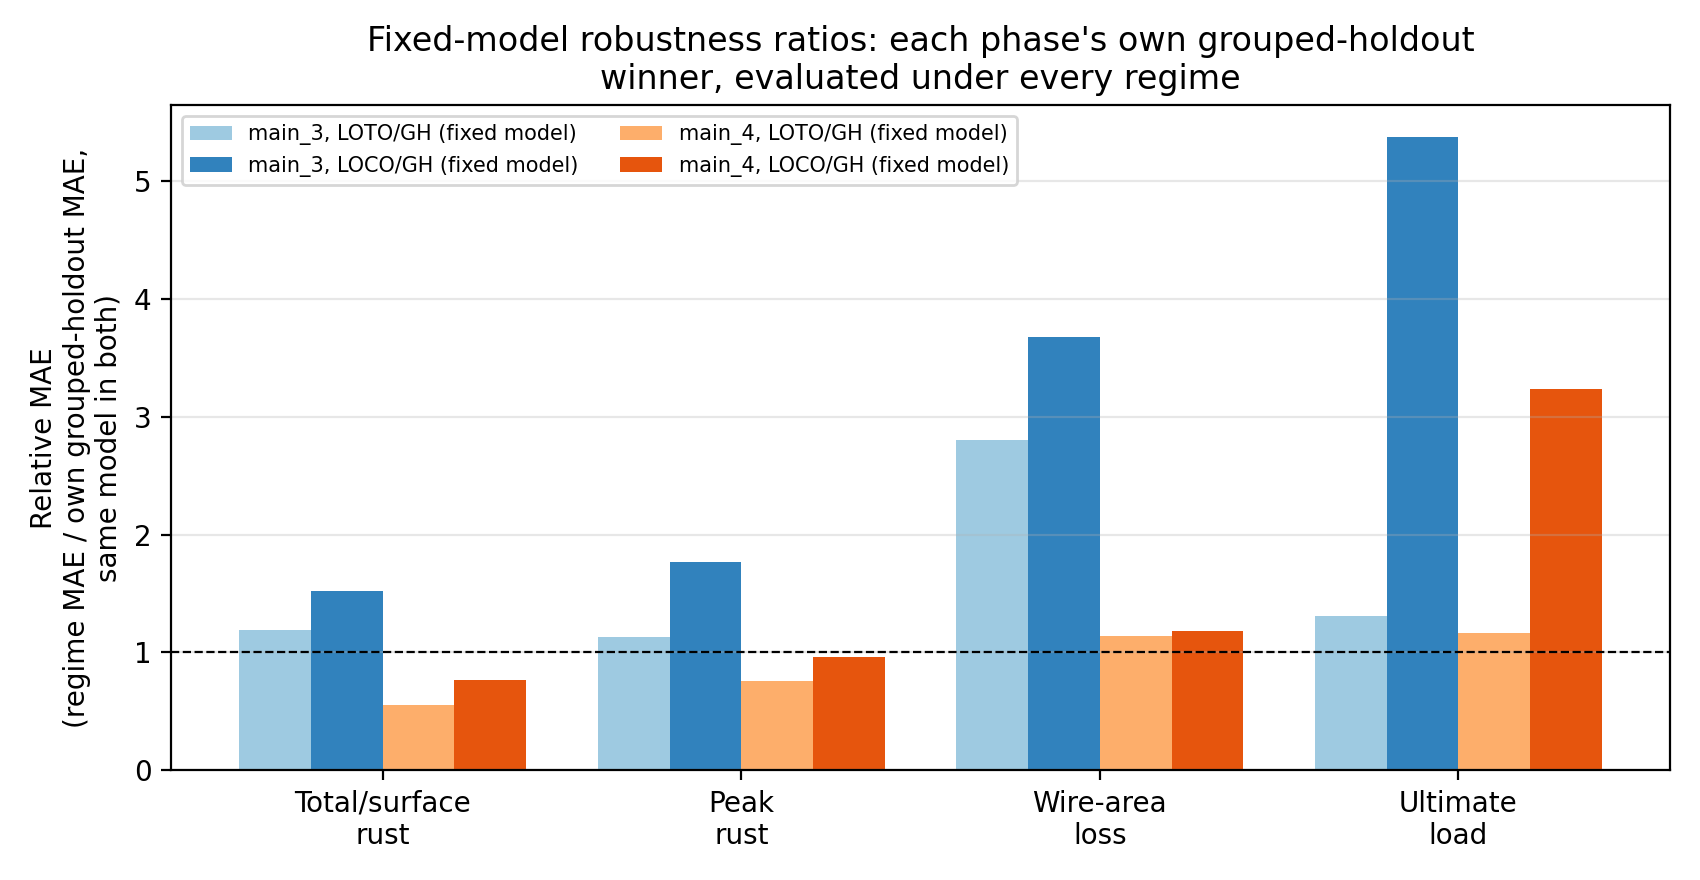
\includegraphics[width=0.62\textwidth]{fig_5_1_robustness_synthesis.png}
\caption{Relative MAE (regime MAE divided by that same model's own
grouped-holdout MAE) for the two visible-corrosion and two structural
targets, using each phase's own grouped-holdout-winning model evaluated
under every regime — a fixed-model comparison, not a
best-available-model-per-regime one.\footnote{Fixed models: the
interpretable-feature phase uses RandomForest for total rust, wire-area
loss, and ultimate load, and an MLP for peak rust; the
robustness-quantification phase uses GradientBoosting for surface total
rust and RandomForest for the remaining three targets. The
robustness-quantification phase's benchmark table is computed on this
fixed-model basis by its own diagnostics code; the interpretable-feature
phase's values were recomputed this session using the same rule against
its own saved per-fold metrics.} No raw MAE from one phase is compared
against another phase's raw MAE. Structural targets inflate under both
regimes in both phases, most severely for ultimate load under
leave-one-campaign-out; visible-corrosion targets stay close to or below
their own grouped-holdout MAE under leave-one-campaign-out in both phases,
but diverge under leave-one-treatment-out — fragile in the
interpretable-feature phase, robust in the robustness-quantification
phase.}
\label{fig:results-robustness-synthesis}
\end{figure}

Figure~\ref{fig:results-robustness-synthesis} shows both the replication
and the divergence directly: the structural-target inflation pattern and
the visible-corrosion targets' campaign-level robustness recur
independently across two phases with unrelated feature engineering, which
makes it unlikely that these two patterns are artefacts of a single
phase's feature-engineering choices; the visible-corrosion treatment-level
fragility does not recur, and should be read as specific to the
interpretable-feature phase's own treatment-holdout evaluation rather than
as a property of the data itself.

\section{Degradation and Proxy-RUL Evidence}
\label{sec:results-degradation}

Two generations of the degradation/proxy-RUL derivation
(Section~\ref{sec:proxy-rul}) exist in the project, on configurations that
are not directly comparable. The first
(Section~\ref{sec:phase3-degradation}) fits a composite four-series
derivation — two observed visible-corrosion series and two model-estimated
structural series — against three threshold types over a 104-week
projection horizon: of 48 specimens, 33 receive a finite estimate, 23 of
which are exactly zero weeks, leaving only ten with a proxy-RUL that is
both finite and genuinely forward-looking.

The second generation instead derives threshold-crossing status from a
single series (model-estimated wire-area-loss fraction) against three
absolute thresholds over a shorter, 365-day horizon — a narrower target
and a materially different horizon, so the two are compared here only at
the level of their conclusions, not their counts. Its own saved output
classifies every one of the 144 specimen/threshold combinations tested as
already past the threshold at the first observation, crossed during
observation, or not crossed within the horizon: there is no genuinely
forward-looking finite crossing anywhere in this refined output, a still
more conservative result than the first generation's ten forward-looking
cases. The project's own documentation separately flags, as an unresolved
validation concern rather than a confirmed defect, that most specimens
already show a model-estimated wire-area loss at or above the lowest
threshold at their first observation — consistent with most crossings
being attributed to the baseline rather than to projected degradation.

\emph{Bounded conclusion:} both generations of the degradation/proxy-RUL
pipeline demonstrate that the derivation chain defined in
Section~\ref{sec:proxy-rul} can be executed end to end, and both
generations' own outputs argue against treating the resulting numbers as
validated remaining-life estimates: the first because most of its finite
estimates are degenerate, the second because it produces no forward-looking
estimate at all under a more conservative configuration. True remaining
useful life remains unavailable in this dataset regardless of which
generation is consulted.

\section{Current Four-Class Classification Branch}
\label{sec:results-classification}

The four-class classification effort (Section~\ref{sec:phase5}) is
structurally independent of every modelling question addressed above: it
targets a different task (discrete severity classification rather than
continuous estimation), a different, current four-level schema
(Table~\ref{tab:category-schema}), and shares no code with any earlier
phase. Data preparation for this task is complete and verified: the target
schema, the class-imbalance characterisation, the specimen-level grouped
split, the leakage-safety runtime check, and the augmentation pipeline all
exist and have been run. No classifier has been trained, compared, or
evaluated on this data at the time of writing. This branch therefore
contributes methodology and data-preparation evidence to this report, not
model-performance evidence, and it is not compared against the
interpretable-feature phase's five-category classification results
(Section~\ref{sec:phase3-corrosion}), which model a different, historical
schema with a different number of classes.

\section{Integrated Findings}
\label{sec:results-integrated}

Table~\ref{tab:cross-phase-comparability} summarises which quantitative
results in this project may be compared directly, which may only be
compared as ratios to their own baseline, and which must be compared only
qualitatively. Table~\ref{tab:integrated-findings} then states, for each
scientific question addressed in this chapter, the project's current
evidence level, main finding, main limitation, and the most defensible
claim the evidence supports. Evidence-level terms are used as defined in
the surrounding text of this chapter and are not numeric scores: \emph{well
supported} indicates a conclusion replicated across phases and stable under
at least one stricter evaluation regime; \emph{conditionally supported}
indicates a conclusion that holds under some but not all tested conditions;
\emph{exploratory} indicates a working demonstration not yet validated
against an independent standard; \emph{not yet evaluated} indicates that no
model-performance evidence exists at all.

\begin{table}[htbp]
\centering
\caption{Cross-phase comparability. What may be compared directly, as a
ratio to each result's own baseline, or only qualitatively, and why.}
\label{tab:cross-phase-comparability}
\small
\begin{tabular}{p{3.2cm}p{3.3cm}p{6.0cm}}
\toprule
Comparison & Permitted form & Reason \\
\midrule
Interpretable-feature phase vs.\ robustness-quantification phase, same
target family, robustness pattern & Ratio (regime MAE / own
grouped-holdout MAE) or qualitative & Different feature sets and dataset
bases (792 vs.\ 791 rows); absolute MAE not comparable, but both phases
independently test the same robustness question. \\
Classical baseline vs.\ interpretable-feature phase, current-corrosion
accuracy & Qualitative only & Different feature engineering, different
label-construction tautology risk (Section~\ref{sec:results-visible}); not
placed on a shared ranked list. \\
Interpretable-feature phase vs.\ terminal-load-focused phase, ultimate-load
MAE & Not compared numerically & Different feature sets, splits, and
dataset bases (Section~\ref{sec:phase3-structural}); comparing 0.121~kN
against 0.174~kN as a leaderboard would be a category error. \\
Deep-embedding phase vs.\ terminal-load-focused phase, image value & Not
compared numerically & Different targets (current-week peak rust vs.\
terminal ultimate load) and different representations; deep-embedding
phase lacks a metadata-only baseline (Section~\ref{sec:results-incremental}). \\
First-generation vs.\ second-generation proxy-RUL & Qualitative (both
support the same bounded conclusion) & Different target composition,
threshold definitions, and projection horizons (104 weeks $\approx$ 728
days versus 365 days $\approx$ 52 weeks;
Section~\ref{sec:results-degradation}). \\
Historical five-class classification (interpretable-feature phase) vs.\
current four-class classification & Not compared & Different category
schema (Table~\ref{tab:category-schema}); the current branch has no
trained-model result to compare. \\
\bottomrule
\end{tabular}
\end{table}

\FloatBarrier

\begin{table}[htbp]
\centering
\caption{Integrated scientific findings across the project. Evidence-level
terms are defined in the surrounding text and are not numeric scores.}
\label{tab:integrated-findings}
\footnotesize
\begin{tabular}{p{2.5cm}p{1.9cm}p{3.3cm}p{3.3cm}}
\toprule
Question & Evidence level & Main finding & Defensible claim \\
\midrule
Visible surface corrosion (Section~\ref{sec:results-visible}) & Well
supported (peak rust; campaign-level robustness); conditionally supported
(total rust, tautology risk; treatment-level robustness, phase-dependent)
& Robust under campaign holdout in both phases; treatment-holdout
robustness diverges between phases (fragile in one, robust in the other)
& Images carry genuine, learnable visible-corrosion signal, most credibly
for peak rust, robust under campaign-level transfer; treatment-level
transfer is unresolved, not established as a project-wide weakness \\
Hidden structural condition (Section~\ref{sec:results-structural}) &
Conditionally supported, weak & Grouped-holdout signal collapses under
both stricter regimes; final selected models are metadata-only & The
evidence supports substantially weaker structural inference than visible-
corrosion inference; not established that images cannot help in
principle \\
Terminal ultimate load / incremental image value
(Section~\ref{sec:results-incremental}) & Conditionally supported (against
image value) & Metadata-only is the strongest pooled predictor; a narrow
post-onset exception exists & Images do not add a reliable pooled
improvement over metadata for terminal ultimate load \\
Cross-regime / cross-campaign robustness (Section~\ref{sec:results-robustness})
& Well supported (campaign-level pattern; structural fragility);
conditionally supported (treatment-level visible-corrosion behaviour,
phase-dependent) & Structural fragility under both stricter regimes, and
visible-corrosion robustness under campaign holdout, replicate across two
phases; treatment-holdout behaviour for visible-corrosion diverges between
phases & Robustness behaviour is target-family- and regime-specific;
campaign-level and structural findings replicate across phases, but
treatment-level visible-corrosion robustness does not and should be
treated as phase-dependent \\
Degradation / proxy-RUL (Section~\ref{sec:results-degradation}) &
Exploratory & Derivation chain executable end to end in two non-comparable
configurations; both argue against forward-looking confidence & Useful as
an exploratory screening framework; not a validated remaining-life
estimate \\
Four-class classification (Section~\ref{sec:results-classification}) & Not
yet evaluated & Data preparation, splitting, and augmentation complete; no
classifier trained & Contributes methodology evidence only; no
performance claim can yet be made \\
\bottomrule
\end{tabular}
\end{table}

\FloatBarrier

Read together, these rows describe a project whose strongest evidence
concerns visible-corrosion estimation, reinforced across independent
phases except for treatment-level robustness, which is phase-specific
rather than replicated (Section~\ref{sec:results-robustness}). Its most
consequential negative findings were established in different ways and
should not be flattened into one narrative of replication: campaign-
confounded structural supervision was named early and reinforced by later,
independent requantification (Sections~\ref{sec:results-structural}
and~\ref{sec:phase4a}); proxy-RUL's non-validated status is reinforced by
two independently configured generations of the same derivation
(Section~\ref{sec:results-degradation}); but the absence of reliable
incremental image value for terminal ultimate load rests on one phase's
own designed three-way ablation
(Section~\ref{sec:results-incremental}), not on independent replication by
a separate experiment, and is best read as a single well-designed test
rather than a cross-phase-confirmed pattern.


% =============================================================
% Chapter 6 -- Scientific Interpretation and Research Decisions
% =============================================================
\chapter{Scientific Interpretation and Research Decisions}
\label{ch:interpretation}

Chapter~\ref{ch:activities} described what was built; Chapter~\ref{ch:results}
established what the integrated evidence shows. This chapter asks what
those findings mean scientifically, and why they justified the major
research decisions the project actually took. It does not repeat the
chronological narrative or the metric-by-metric synthesis of the two
preceding chapters; results are cited by reference, briefly, only where a
specific number is the direct subject of an interpretive claim. This
chapter distinguishes throughout between what the evidence supports
observing and what may be inferred from it, and prefers hedged language
("is consistent with," "suggests," "cannot distinguish between") to
causal claims wherever a causal mechanism is not established by the
project's or the predecessor's own documentation.

\section{From Visible Corrosion to Structural Condition: An Evidence Hierarchy}
\label{sec:interp-hierarchy}

The project's successive research questions form an evidence hierarchy,
not a sequence of independent tasks — and not a literal universal
computational pipeline in which each stage is generated exclusively from
the stage immediately above it. Figure~\ref{fig:evidence-hierarchy} sets
this out as a ladder of increasing inferential distance from directly
observed quantities, decreasing supervision density, and increasing
dependence on modelling assumptions; actual feature inputs at each stage
are phase-dependent, not fixed by the ladder position alone. Direct
observations and labels — images, visible-corrosion labels, and
specimen/exposure metadata — sit at the top, densely available for nearly
every observation (Section~\ref{sec:data-modalities}). Image
representations and image-based estimates are computed from these
observations. Hidden structural condition is a model's estimate, fit on 48
terminal measurements and applied to weeks at which no structural
measurement exists (Section~\ref{sec:structural-supervision}); its actual
inputs vary by phase rather than depending on the image-
representation tier alone — the interpretable-feature phase's structural
models are mixed-input (metadata, manually assigned corrosion labels, and
image descriptors together), while the robustness-quantification phase's
final selections use metadata only (Section~\ref{sec:results-structural}).
Degradation trajectories are curves fitted to those estimated, not
measured, series (Section~\ref{sec:phase3-degradation}). Proxy-RUL is a
threshold-crossing time read off an extrapolation of one of those fitted
curves (Section~\ref{sec:proxy-rul}).

\begin{figure}[htbp]
\centering
\resizebox{0.85\textwidth}{!}{% Report schematic (conceptual diagram, not a measured result / not to
% scale, and not a computational data-flow diagram). Position in this
% ladder reflects increasing inferential distance from directly observed
% quantities, decreasing supervision density, and increasing dependence on
% modelling assumptions -- it does NOT mean that each stage is computed
% exclusively from the stage immediately above it. Actual feature inputs
% are phase-dependent: e.g. hidden structural estimates in one phase are
% mixed-input (metadata + manually assigned corrosion labels + image
% descriptors), while another phase's final structural selections are
% metadata-only. Plain connecting lines (no arrowheads) are used
% deliberately, to avoid implying a universal computational dependency.
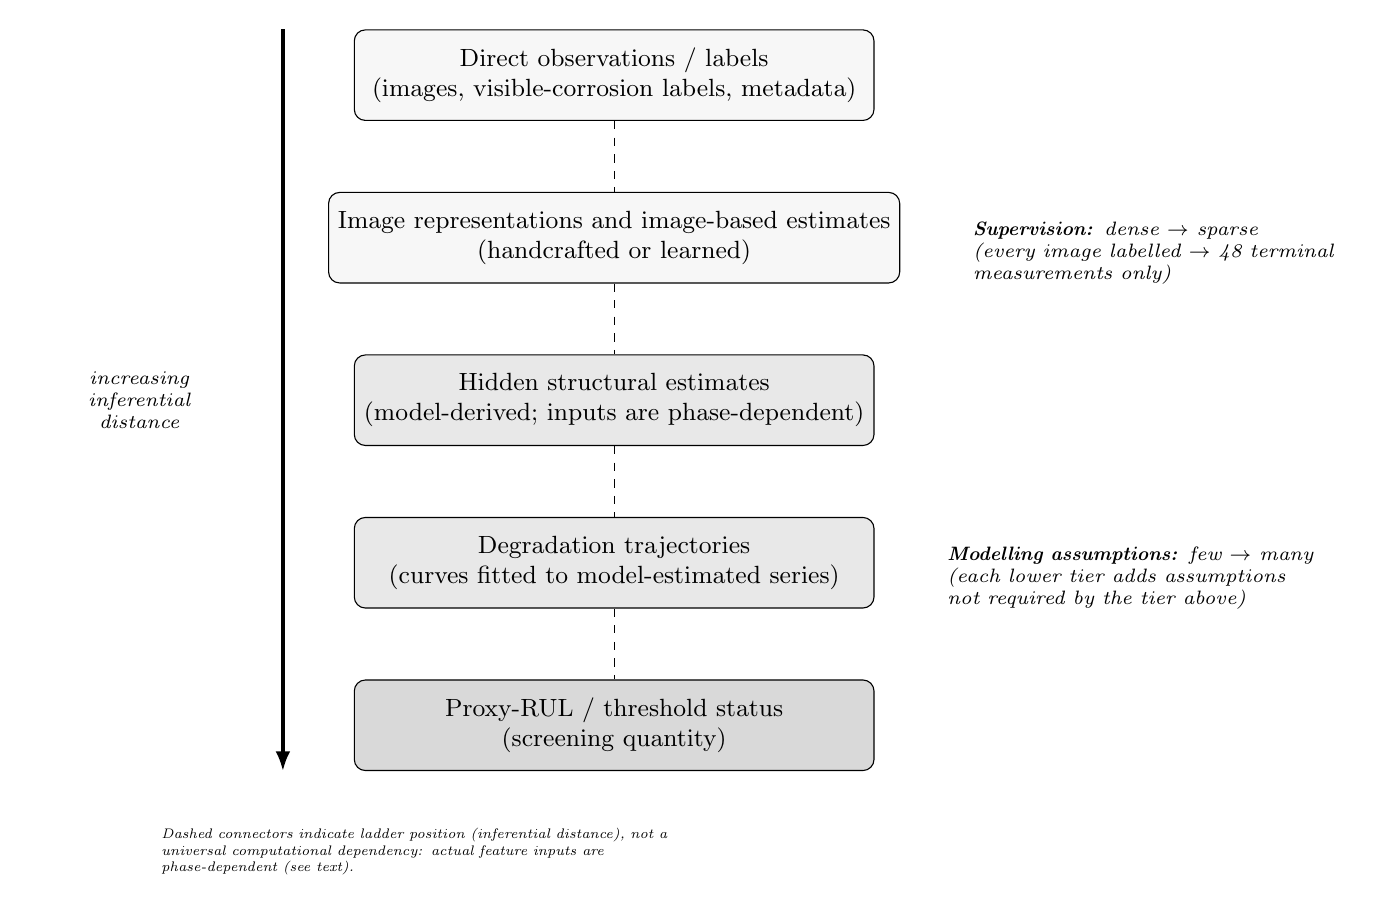
\begin{tikzpicture}[
    node distance=9mm and 10mm,
    stage/.style={draw, rounded corners, align=center, minimum width=6.6cm,
                minimum height=1.15cm, font=\small},
    observed/.style={stage, fill=gray!6},
    derived/.style={stage, fill=gray!18},
    screening/.style={stage, fill=gray!30},
    conn/.style={thin, dashed},
    bracket/.style={very thick, -{Latex[length=2.5mm]}},
    sidelbl/.style={font=\scriptsize\itshape, align=left}
]

\node[observed] (obs) {Direct observations / labels\\(images, visible-corrosion labels, metadata)};
\node[observed, below=of obs] (images) {Image representations and image-based estimates\\(handcrafted or learned)};
\node[derived, below=of images] (structural) {Hidden structural estimates\\(model-derived; inputs are phase-dependent)};
\node[derived, below=of structural] (trajectory) {Degradation trajectories\\(curves fitted to model-estimated series)};
\node[screening, below=of trajectory] (rul) {Proxy-RUL / threshold status\\(screening quantity)};

\draw[conn] (obs) -- (images);
\draw[conn] (images) -- (structural);
\draw[conn] (structural) -- (trajectory);
\draw[conn] (trajectory) -- (rul);

\draw[bracket] ([xshift=-9mm]obs.north west) -- ([xshift=-9mm]rul.south west);

\node[sidelbl, left=13mm of structural, text width=2.6cm, align=center]
  {increasing\\inferential\\distance};

\node[sidelbl, right=8mm of images, yshift=-2mm, text width=4.8cm]
  {\textbf{Supervision:} dense $\rightarrow$ sparse\\(every image labelled $\rightarrow$ 48 terminal measurements only)};
\node[sidelbl, right=8mm of trajectory, yshift=-2mm, text width=4.8cm]
  {\textbf{Modelling assumptions:} few $\rightarrow$ many\\(each lower tier adds assumptions not required by the tier above)};

\node[font=\tiny\itshape, align=left, below=6mm of rul, text width=11.5cm]
  {Dashed connectors indicate ladder position (inferential distance), not a\\
   universal computational dependency: actual feature inputs are\\
   phase-dependent (see text).};

\end{tikzpicture}
}
\caption{Conceptual report schematic (not a measured result). Position in
the ladder reflects increasing inferential distance from directly observed
quantities, decreasing supervision density, and increasing dependence on
modelling assumptions — not a universal computational dependency in which
each stage is generated solely from the stage immediately above it; actual
feature inputs are phase-dependent, as discussed in the surrounding text.
This illustrates why evidential confidence decreases downstream, not that
downstream estimation is impossible.}
\label{fig:evidence-hierarchy}
\end{figure}

This hierarchy is offered as an organising explanation for a pattern
already established in Chapter~\ref{ch:results}: results become
progressively less robust and more heavily qualified moving down it.
That pattern is consistent with supervision becoming sparser and model
dependence compounding at each step; it is not, on its own, proof that any
particular downstream quantity cannot in principle be estimated more
reliably with different data or methods. The distinction matters for how
the rest of this chapter should be read: each section below interprets why
the evidence looks the way it does, without treating the hierarchy itself
as an argument for impossibility.

\section{Why Visible Corrosion Was the Strongest Image-Based Task}
\label{sec:interp-visible}

Three independent phases, using unrelated representations (a fixed colour
threshold, a frozen deep embedding, and an explicitly engineered
multi-family feature set), each reached useful grouped-holdout accuracy
for a visible-corrosion target (Section~\ref{sec:results-visible}). This
consistency across unrelated representations is consistent with the
underlying task being genuinely well suited to image-based estimation:
corrosion is a surface phenomenon that manifests directly in the
photographic record, and it is the one target family labelled at the same
fine time resolution as the images themselves
(Section~\ref{sec:data-modalities}), giving every phase far more
supervision to learn from than any structural target could offer.

This should not, however, be read as a uniform success story. Peak rust
provides more meaningful independent evidence of genuine image-driven
estimation than the total-rust benchmarks do, precisely because two
separate phases independently found total/current rust predictions
dominated by a feature closely aligned with, or nearly identical to, the
label itself (Section~\ref{sec:results-visible}). The lesson this
supports is specific and worth stating plainly: high predictive accuracy
is not sufficient evidence of a learned visual concept if the dominant
feature substantially reconstructs the target's own definition. This
chapter treats that lesson as a general one, applicable beyond the two
cases in which it was directly observed, not as a defect specific to
those two phases. Robustness, similarly, does not transfer uniformly:
campaign-level robustness for visible corrosion is a replicated finding,
while treatment-level robustness is not
(Section~\ref{sec:results-robustness}). The difference may partly reflect
changes in treatment-group definition, size, or composition between the
two implementations; the available evidence establishes the disagreement
itself, not its mechanism, and does not rule out the visual task as a
contributor.

\section{Why Structural Inference Was Harder}
\label{sec:interp-structural}

Hidden structural condition differs from visible corrosion along every
axis identified in Chapter~\ref{ch:dataset}: it is measured once per
specimen rather than repeatedly, at a single terminal timepoint rather
than throughout the observation period, for only 48 specimens rather than
791 observations (Section~\ref{sec:structural-supervision}). This sparse,
single-timepoint supervision is a major limitation consistent with the
observed instability of structural models relative to visible-corrosion
models, independent of any claim about the images themselves. It is
compounded by the experimental design's near-perfect alignment of
campaign identity with steel-mesh configuration, chloride concentration,
and ageing duration (Section~\ref{sec:confounding}): a model trained on
all 48 rows has, in effect, only two campaign-level combinations of the
principal design variables (mesh configuration, chloride level, and
terminal duration) to learn from — treatment variation still exists within
each campaign — and evaluating it under leave-one-campaign-out asks it to
extrapolate to a combination of those variables it has never encountered
(Section~\ref{sec:loco}).

The available evidence supports a narrow, specific conclusion, and it is
important not to overstate it in either direction. It would be wrong to
conclude that surface corrosion does not affect structural capacity — no
result here tests that physical claim directly, and Chapter~\ref{ch:results}
explicitly avoided asserting it. The evidence instead supports the
narrower claim that this dataset and this experimental design do not
isolate a robust, incremental, image-based relationship to hidden
structural capacity. The distinction is between a physical relationship,
which the available evidence can neither confirm nor rule out, and
predictive identifiability from this specific dataset, which is what was
actually tested and what the project's results speak to. Reading the
mixed-input character of the interpretable-feature phase's structural
models alongside the metadata-only character of the robustness-
quantification phase's final selections (Section~\ref{sec:results-structural})
reinforces this reading: even when image descriptors are made available to
a structural model, the model does not consistently rely on them once
selection is made robustness-aware.

\section{Metadata Dominance: Signal or Shortcut?}
\label{sec:interp-metadata}

Metadata's dominance of the terminal-load prediction task
(Section~\ref{sec:results-incremental}) admits two readings that hold
simultaneously rather than competing. Steel-mesh configuration, chloride
exposure, ageing duration, and treatment protocol are genuine design and
exposure variables with a plausible physical relationship to structural
response; there is nothing suspect, in itself, about a model finding them
predictive. At the same time, because these same variables are almost
perfectly aligned with campaign identity in this sample
(Section~\ref{sec:confounding}), a pooled model's reliance on them cannot
be distinguished, from the pooled evidence alone, from the model simply
having learned which campaign a specimen came from. Both readings are
consistent with the same pooled result, and the available evidence does
not adjudicate between them from the pooled analysis alone.

This is why metadata should not be described as invalid or as a nuisance
variable to be engineered away: it may well carry real information about
structural response, and a metadata-only baseline is exactly the right
comparison against which to judge whether images add anything further
(Section~\ref{sec:multimodal}). What the mesh-stratified and campaign-
holdout evidence adds (Section~\ref{sec:results-structural}) is a second,
independent check on the same question, without relying on the pooled
correlation at all. The failure to retain predictive quality within mesh
groups and under campaign holdout weakens the evidence that the pooled
metadata relationship is transferable beyond campaign-linked structure; it
does not disprove a genuine physical metadata effect, only the claim that
the pooled result demonstrates one. This is why pooled predictive
performance can be genuinely useful — it is still the strongest available
baseline for this task — while simultaneously being insufficient evidence,
on its own, of a transferable structural relationship.

\section{Why the Research Question Was Refocused}
\label{sec:interp-refocus}

The shift from hidden-damage estimation toward the terminal ultimate-load
refocus (Section~\ref{sec:phase4b}) is best read as a scientifically
motivated narrowing of claim scope, not as a retreat from a failed
experiment. The hidden-damage chain — estimate structural condition at
every observation week, fit a degradation curve to those estimates,
extrapolate to a threshold crossing — compounds a separate layer of
modelling uncertainty at each step (Section~\ref{sec:results-degradation}).
Terminal ultimate load, by contrast, is directly measured for every one of
the 48 specimens at a single, well-defined timepoint
(Section~\ref{sec:experimental-context}), which removes the need for any
intervening model-estimated quantity between the data and the target.

Reframing the question around that directly measured endpoint also made
the resulting experiment more bounded and directly testable. "Do images
add information beyond known design and exposure metadata for a directly
measured terminal endpoint?" is a bounded, answerable question with a
specific comparison built in from the start (Section~\ref{sec:multimodal}).
"Can a sparse hidden state be estimated at every intermediate week and
then extrapolated into a remaining-life estimate?" is not incoherent, but
is substantially harder to validate and diagnose, because disagreement at
the final stage cannot be cleanly attributed to one component without
independent intermediate ground truth. The refocused study's own
design — matched feature-set comparisons, a mesh-stratified check, and a
campaign-holdout stress test, all reported together rather than as a
single isolated accuracy number (Section~\ref{sec:phase4b}) — is
consistent with this being a stronger experimental design, not merely a
narrower one.

\section{Scientific Value of the Negative Results}
\label{sec:interp-negative}

Several of the project's most useful findings are negative, and they
should be read as evidence, not as failures to be minimised. That images
do not provide a reliable pooled improvement over metadata for terminal
ultimate load (Section~\ref{sec:results-incremental}) provides evidence
against an otherwise plausible claim in this dataset, under the tested
pooled setting, rather than merely failing to confirm it. That
every feature-set configuration achieves negative $R^2$ within a single
mesh family (Section~\ref{sec:phase4b}) reveals a gap between absolute
error and explained variance that a less careful evaluation would have
missed entirely. That structural performance collapses under
leave-one-campaign-out in every phase that tested it
(Section~\ref{sec:results-structural}) identifies exactly which evaluation
regime future work in this dataset must budget for. That the refined
proxy-RUL configuration yields a zero future-crossings result — no
projected future threshold crossing among any of the tested cases, even
though many are already crossed at baseline or during observation
(Section~\ref{sec:results-degradation}) — is a more informative outcome
than a handful of plausible-looking but unvalidated future estimates would
have been. That the residual-correction attempt on
top of the metadata-only baseline measurably worsened performance
(Section~\ref{sec:phase4b}) was recorded rather than discarded, which is
itself part of what makes the surrounding positive claims credible. Each
of these findings narrows the space of defensible claims, exposes a
specific confound or data requirement, and motivates a specific next
check — which is what a negative result is for.

\section{What the Proxy-RUL Work Contributes}
\label{sec:interp-rul}

The proxy-RUL pipeline's contribution is methodological and diagnostic,
not prognostic, and this chapter states that distinction directly rather
than qualifying it away. Executing the four-step derivation end to end,
twice, under two independently configured settings
(Section~\ref{sec:results-degradation}), forced an explicit separation
between observed and model-estimated condition series
(Table~\ref{tab:quantity-availability}) that a less disciplined pipeline
could have left implicit. The refined generation's threshold-status
taxonomy — crossed at baseline, crossed during observation, or not crossed
within the horizon — is a more transparent way of reporting the same
underlying uncertainty than a single ambiguous "weeks remaining" figure
would be, and its own zero future-crossings result is itself a diagnostic
finding: the absence of any projected future crossing, together with the
large number of already-baseline-crossed cases, is consistent with
threshold status being strongly influenced by already-elevated baseline
structural estimates, although that decomposition was not itself
quantified. The physical plausibility of those baseline structural
estimates remains, by the project's own account, an unresolved validation
check rather than a settled fact. The project's own supporting
documentation separately and explicitly recommends exporting genuinely
held-out (out-of-fold) structural predictions in place of the current
in-sample refits for any future degradation-modelling work — naming the
relevant risk directly: that degradation and proxy outputs built on
in-sample structural refits can appear more confident than the underlying
structural model's own robustness evidence would justify. This is a
downstream-optimism risk the project's own documentation makes visible,
not one this chapter is introducing for the first time.

None of this amounts to validated remaining-life estimation, and the
project's own dataset does not support it: true RUL validation would
require either a recorded failure-event time or repeated, rather than
single-terminal, structural measurements per specimen
(Section~\ref{sec:proxy-rul}), and neither is present. The pipeline's
value lies in having built, tested, and critically examined the
derivation chain that such data would require — clarifying exactly what
is still missing — rather than in having produced a usable service-life
number.

\section{Interpretation of the Four-Class Classification Direction}
\label{sec:interp-classification}

The current four-class classification effort is a reasonable next
direction on methodological grounds, independent of what a future trained
classifier will show. It targets a directly observable quantity — image to
severity category — rather than a model-derived or extrapolated one,
using an explicit, current schema kept distinct from the historical
five-level scheme used in the earlier dataset build
(Section~\ref{sec:dataset-audit}). Its
class imbalance was characterised before any training was attempted
(Section~\ref{sec:phase5}), its specimen-level grouped split and leakage-
safety runtime check were implemented and verified rather than merely
documented, and its augmentation recipes were chosen or rejected on stated
physical-plausibility grounds rather than convenience. Read together,
these choices show the branch incorporating, from the outset, the
methodological lessons the earlier regression work had to establish
one at a time over several phases (Section~\ref{sec:interp-lessons}) —
which is a reasonable basis for describing it as well prepared, whatever
its eventual accuracy turns out to be.

This should not be read as more than it is. No classifier has been
trained, compared, or evaluated on this data, and no ResNet-50 or Vision
Transformer experiment exists yet in this project
(Section~\ref{sec:results-classification}). The evaluation practice
already specified for whichever training procedure is used next —
macro-averaged F1 and per-class recall in preference to overall accuracy,
given the severity of the class imbalance, and a test partition left
untouched until final evaluation (Section~\ref{sec:metrics}) — is stated
here as the standard this branch should be held to, not as a result
already obtained.

\section{Methodological Lessons}
\label{sec:interp-lessons}

Several lessons recur across the sections above and are worth drawing
together briefly, as a closing statement rather than a scorecard. Evaluation design can matter more than model complexity: the
project's regime comparisons changed which results were credible more
than any change of model family did (Section~\ref{sec:interp-visible},
Section~\ref{sec:eval-regimes}). A grouped holdout is necessary but not
sufficient: it answers a narrower question than transfer to a new
treatment or campaign, and the project's own later phases treated
additional regimes as required, not optional
(Section~\ref{sec:principles}). Accuracy without attention to target
provenance can be actively misleading, as the total-rust and peak-rust
contrast shows directly (Section~\ref{sec:interp-visible}). A metadata-only
baseline is not an optional control but a precondition for any claim that
images add value (Section~\ref{sec:interp-metadata}). Sparse downstream
labels bound what any model, however capable, can be shown to establish,
independent of modelling effort (Section~\ref{sec:interp-structural}).
Negative results are informative and should shape the next question rather
than be minimised or omitted (Section~\ref{sec:interp-negative}). And
where a directly measured endpoint exists, it is preferable to a longer
chain of model-derived proxies for exactly the reason the terminal-load
refocus illustrates: each additional derived step is an additional,
separately uncertain modelling assumption
(Section~\ref{sec:interp-refocus}).

These lessons are offered as this project's own accumulated methodological
position, consistent with the evidence reviewed in
Chapters~\ref{ch:activities} and~\ref{ch:results}, rather than as general
claims about machine learning practice beyond this project's scope.


% =============================================================
% Chapters 7-9 -- Software Engineering, Limitations, Status
% =============================================================
\chapter{Software Engineering, Reproducibility, and Project Infrastructure}
\label{ch:engineering}

This chapter documents how the project's codebase was organised and made
progressively more traceable, and states plainly which concrete engineering
issues currently limit a clean rerun of parts of it. It is not a tutorial
on version control, configuration formats, or machine-learning tooling in
general; every claim below is specific to this repository, with an exact
file or artifact cited.

\section{Repository and Pipeline Evolution}
\label{sec:eng-evolution}

The project's codebase falls into three engineering tiers. The
exploratory prototype (\texttt{main\_first}, Section~\ref{sec:phase0}) is
a small set of unparameterised scripts with no configuration layer, no
persisted metrics, and no held-out evaluation at all — its defining
engineering weakness, not merely a scientific one. Four successive,
increasingly structured modelling generations follow it:
\texttt{main}, \texttt{main\_2}, \texttt{main\_3}, and \texttt{main\_4}.
The earliest of these four still parameterise thresholds and paths
directly in training scripts. \texttt{main\_3} introduces a single
centralised configuration file (\texttt{configs/default.toml}) for its
degradation and RUL thresholds. \texttt{main\_4} completes this shift: six
YAML configuration files (\texttt{dataset}, \texttt{features},
\texttt{modeling}, \texttt{thresholds}, \texttt{specimen\_mapping},
\texttt{ultimate\_load\_refocus}) are loaded through one function and
cached (\texttt{config.py}), so that a model-selection weight, a
threshold, or a random seed is changed in one place rather than in
scattered script arguments. \texttt{augmentation} is a later, separate
branch built for the four-class classification effort
(Section~\ref{sec:phase5}), following the same or greater configuration and
leakage-safety discipline as \texttt{main\_4}. Across all four modelling
generations, source, configuration, and generated output become more
consistently separated into distinct directories (\texttt{src/},
\texttt{configs/}, \texttt{outputs/}), and metrics, split manifests, and
diagnostic tables are persisted as saved artifacts rather than console
output.

\section{Data and Artifact Provenance}
\label{sec:eng-provenance}

The mature pipeline's artifact chain runs from raw workbook and image
files, through an aligned/canonical data table, to extracted features,
saved split manifests, model metrics and predictions, and finally to the
figures and tables cited in this report. This chain is traceable but not
uniformly automated across every phase: \texttt{main\_4}'s
\texttt{outputs/} tree separates \texttt{data/}, \texttt{models/}, and
\texttt{diagnostics/} consistently, while the earlier \texttt{main} and
\texttt{main\_2} phases save flatter \texttt{reports/} directories with
less internal structure. The single canonical source for campaign,
treatment, mesh, and chloride facts is \texttt{configs/specimen\_mapping.yaml}
(Section~\ref{sec:experimental-context}), used in preference to raw
workbook columns precisely because it is a single, version-controlled
table rather than a value re-derived independently in each script. This
report's own \texttt{evidence\_log.md} and per-chapter evidence-plan files
extend that same provenance discipline one level further, recording the
exact source file, tier, and caveat behind every number cited in
Chapters~\ref{ch:activities}--\ref{ch:interpretation}.

\section{Split and Evaluation Reproducibility}
\label{sec:eng-splits}

Whether another researcher can identify which observations belong to which
partition — not what the partitions mean scientifically, already covered
in Section~\ref{sec:eval-regimes} — depends on concrete, checkable
artifacts. The classification/augmentation effort's train, validation, and
test manifests are saved as explicit CSV files
(\texttt{Data/splits/\{train,val,test\}\_manifest.csv}), and specimen
assignment to validation and test is fixed by hardcoded, disjointness-checked
specimen-ID lists rather than by a random draw; \texttt{make\_splits.py}
raises a \texttt{RuntimeError} if those lists overlap, if any augmented
image is found outside the training partition, or if a specimen appears in
more than one split. The regression phases' grouped-holdout, LOTO, and
LOCO folds are reproducible in a weaker sense: \texttt{main\_4} records an
explicit \texttt{random\_state: 42} in its modelling configuration files,
and per-fold split summaries are saved under \texttt{outputs/splits/}, but
the fold assignments themselves depend on the installed scikit-learn
version's group-splitting implementation rather than being persisted as an
independent manifest the way the classification splits are.

\section{Image and Feature Reproducibility}
\label{sec:eng-features}

The corrupted-image handling already documented in
Table~\ref{tab:corruption-handling} is itself a reproducibility fact worth
restating in engineering terms: three different policies (drop, impute,
exclude) were applied across five implementation phases, so the row count
a script produces depends on which phase's code is run, and this is a
version-specific property of each phase rather than something to
harmonise after the fact. Feature provenance is otherwise traceable at the
level of saved tables rather than individual descriptors: this report does
not enumerate the ninety-one engineered features of the interpretable
multi-family phase, and instead cites the saved feature tables and the
automated feature-diagnostics report (Section~\ref{sec:eng-contracts})
that characterise them in aggregate. Every new figure this report
generates reads its input directly from a saved project CSV or parquet
file, documented in \texttt{activity\_report/figures/generated\_scripts/}
and cross-verified against the source table rather than transcribed by
hand (Chapters~\ref{ch:activities}--\ref{ch:results}, evidence log).

\section{Configuration and Schema Issues}
\label{sec:eng-schema}

Two distinct, currently live issues were found in the repository's source
and configuration files, verified directly this session; a third,
superficially similar pattern is a legitimate versioned change and must
not be confused with either.

\textbf{(A) A YAML boolean-parsing bug.}
\texttt{main\_4/configs/specimen\_mapping.yaml} records the no-treatment
control protocol as an unquoted \texttt{treatment\_coarse: NO}. Under
PyYAML's default resolver, the bare token \texttt{NO} is a YAML~1.1
boolean literal and is loaded as Python's \texttt{False}, not the string
\texttt{"NO"}. This is directly visible in the generated data: the
\texttt{treatment\_coarse} column of \texttt{outputs/data/master\_table.csv}
contains the literal string \texttt{"False"} for all 168 rows belonging to
the ten no-treatment specimens, while the parallel \texttt{treatment\_raw}
column correctly reads \texttt{"NO"} for the same rows, and the
\texttt{treatment\_protocol} field (\texttt{no\_treatment\_control}) is
unaffected throughout. This is a data-cleanliness and reproducibility
defect in one derived column, not a scientific-result failure: every
treatment-protocol table in this report (Table~\ref{tab:campaign-design})
was built from the unaffected fields, and the bug does not alter any
already-reported count or result.

\textbf{(B) A "1"/"first" $\rightarrow$ "main\_first" string-substitution
pattern, broader than previously logged.} Wherever the current source
tree should contain the standalone numeral \texttt{1} or the word
\texttt{first}, it frequently instead contains the string
\texttt{main\_first}. This was previously known only in two files, in
category-range strings such as \texttt{"A\_Total\_Rust\_Category\_(1--4)"}
appearing as \texttt{"(main\_first--4)"}. Re-verification this session
shows the pattern is substantially wider: it also replaces the pandas
aggregation-function name \texttt{"first"} in named-aggregation and
pivot-table calls across \texttt{main\_2}, \texttt{main\_3}, and
\texttt{main\_4} — directly confirmed to raise
\texttt{AttributeError: 'SeriesGroupBy' object has no attribute
'main\_first'} if such a call is executed today — and it replaces bare
numeral hyperparameter values in \texttt{main\_4}'s YAML configuration
files (for example \texttt{n\_jobs: -main\_first}, \texttt{reg\_lambda:
main\_first.0}, \texttt{glcm\_distances: [main\_first, 3]}), several of
which would fail type validation if the affected pipeline stage were
re-run unmodified. It also appears, harmlessly, in a package version
string (\texttt{"0.main\_first.0"}, which does not prevent the package
from importing) and in comments, docstrings, and generated report prose.
The pattern is confirmed present in \texttt{main}, \texttt{main\_2},
\texttt{main\_3}, and \texttt{main\_4}, and confirmed absent from
\texttt{augmentation}, the most recently written sub-project. Most
affected files across \texttt{main\_3} and \texttt{main\_4} share an
identical modification timestamp, and two files in \texttt{main} share a
second, later timestamp. The saved scientific-output artifacts (metrics,
predictions, and diagnostic tables) from these four affected pipeline
generations that underpin the results reported in
Chapters~\ref{ch:activities}--\ref{ch:interpretation} were re-checked
directly this session — more than two dozen files, dated 2026-03-06 to
2026-03-25 — and all predate both corruption timestamps. This does not
extend to every configuration or documentation file in the repository:
\texttt{specimen\_mapping.yaml} itself carries the later corruption
timestamp, though the specific fields this report cites from it (treatment
protocol, mesh count, chloride level, campaign and terminal-week
identifiers) are not among the affected tokens, which in this file are
confined to a top-level version string and five narrative
\texttt{series\_description} fields not otherwise cited. This clustering
is reported as an observation, not an explanation: the mechanism and cause
of the substitution are not established by the available evidence and are
not claimed here.

\textbf{(C) The four-class/five-class category-schema difference
(Table~\ref{tab:category-schema}) is not an instance of (A) or (B).} It is
a verified, genuine change in the underlying workbook snapshot between two
dataset builds, already established in Chapter~\ref{ch:dataset}, and
should not be reinterpreted as a manifestation of the string-substitution
pattern merely because both happen to involve small integers.

\section{Model and Artifact Contract Limitations}
\label{sec:eng-contracts}

\texttt{main\_4/NEXT\_STEPS\_PLAN.md} independently lists five concrete
engineering improvements; re-checking each against the current repository
this session, rather than assuming the list is uniformly outstanding,
gives a mixed picture. Saving the exact feature list used by each trained
model is only partially done: one global list exists for the hidden-damage
stage, but individual \texttt{best\_model.json} files record only a target
name and a model name, with no feature list or hyperparameters, and no
equivalent file exists for the surface stage. Exporting genuinely
held-out, out-of-fold structural predictions as the basis for degradation
modelling is not done: the degradation stage still consumes in-sample
hidden-damage refits (Section~\ref{sec:results-degradation}). An automatic
feature-quality-control report, by contrast, is already implemented and
run — \texttt{FEATURE\_DIAGNOSTICS.md} is generated by
\texttt{diagnostics.py} and covers exactly the checks recommended
(near-constant, duplicate, and high-collinearity columns). Separating
analysis tables from model-ready feature matrices is not done: the saved
\texttt{surface\_feature\_table.csv} still mixes features, targets, and
identifiers in one file. Saving raw alongside monotone-smoothed
degradation trajectories, initially assumed outstanding, is in fact
already done: \texttt{degradation\_raw\_vs\_monotone\_proxy.csv} stores
both series together.

\section{Reproducibility Improvements Already Achieved}
\label{sec:eng-achieved}

Set against the issues above, several reproducibility practices are
genuinely implemented, not merely recommended, and this chapter closes by
stating them without overclaiming push-button reproducibility for the
project as a whole. Implemented: the current 791-row alignment policy and
its documented rationale (Section~\ref{sec:dataset-audit}); the specimen-mapping
table as a single canonical source; saved audit facts and split manifests
for the classification branch; the automated feature-diagnostics report;
a deterministic, hash-derived augmentation seed whose value is recorded in
the augmentation pipeline's own generated report; a leakage-safety runtime
check enforced in code rather than documented as a convention; and this
report's own figure-generation scripts and evidence log. Recommended but
not yet implemented: an exported dependency specification for
\texttt{main\_4}; correcting the two configuration issues in
Section~\ref{sec:eng-schema}; and the two still-open artifact-contract
items in Section~\ref{sec:eng-contracts}. Given that live configuration
and source corruption is confirmed present in \texttt{main\_4} today, this
chapter does not claim that the repository, as currently checked out, can
be rerun end to end without modification — only that the specific gaps
preventing this are identified, located, and, in most cases, narrow and
fixable.

\chapter{Limitations}
\label{ch:limitations}

This chapter states the limitations of the evidence and implementation
underlying Chapters~\ref{ch:activities}--\ref{ch:interpretation}, organised
by category rather than by project phase. It does not re-run the results
chapter: each item below is stated once, concisely, with a pointer to
where it was established, and the consequence for what the report can and
cannot claim.

\section{Dataset and Experimental-Design Limitations}
\label{sec:lim-dataset}

Every result in this report ultimately rests on 48 physical specimens
tested across only two experimental campaigns, within which steel-mesh
configuration, chloride concentration, and terminal ageing duration
co-vary almost perfectly (Section~\ref{sec:confounding}). Structural
supervision is available at a single terminal timepoint per specimen, with
no repeated or intermediate structural measurement and no observed
failure-event time (Section~\ref{sec:structural-supervision}). The
photographic record covers external surface appearance only; nothing in
the dataset directly measures internal or subsurface condition at any
non-terminal timepoint. Treatment groups are uneven in size, from two
specimens in the smallest protocol to eighteen in the largest
(Table~\ref{tab:campaign-design}). Together, these properties bound every
downstream claim about structural condition, degradation, or transfer
across campaigns or treatments to what a two-campaign, 48-specimen design
can support — a limitation of the physical experiment this project
inherited, not of the modelling choices made within it.

\section{Label and Target Limitations}
\label{sec:lim-labels}

Visible-corrosion labels are manually assigned quantities
(Section~\ref{sec:data-modalities}), not an independent instrumental
ground truth, and two independent findings show that a benchmark built
against them can be label-adjacent rather than purely image-driven: the
classical baseline's peak-rust prediction is dominated by a rust-mask
feature closely aligned with the label (Section~\ref{sec:phase1}), and the
robustness-quantification phase's total-rust benchmark uses a feature
correlated with its label at Spearman $\rho=0.9996$
(Section~\ref{sec:phase4a}). The category schema used for the two
severity targets differs between dataset builds — five ordinal levels
historically, four currently (Table~\ref{tab:category-schema}) — a
genuine version difference in the underlying workbook, not a data-quality
error, but one that prevents any five-class and four-class classification
result from being compared directly. Proxy-RUL thresholds (wire-loss
percentages, a load ratio, a composite health-index cutoff, or the refined
pipeline's single-series thresholds) are engineering screening choices,
not values derived from an independently validated failure criterion
(Section~\ref{sec:proxy-rul}), and no ground-truth remaining-useful-life
value exists anywhere in the dataset against which any of them could be
checked.

\section{Generalisation Limitations}
\label{sec:lim-generalisation}

A grouped specimen holdout answers a narrower question than transfer to a
new treatment or campaign (Section~\ref{sec:grouped-holdout}), and
leave-one-campaign-out in this dataset is better understood as a severe
extrapolation stress test than as an estimate of ordinary future
performance, given how completely campaign identity is entangled with the
principal design variables (Section~\ref{sec:loco}). Treatment-level
(leave-one-treatment-out) behaviour for visible-corrosion targets is not a
settled project-wide property: it is a genuine failure mode in the
interpretable-feature phase and is not reproduced in the
robustness-quantification phase's own treatment-holdout evaluation
(Section~\ref{sec:results-visible}), and the report does not know why.
Within-mesh subgroup analyses are based on only twenty-four specimens per
group (Section~\ref{sec:phase4b}), which limits how much confidence any
single subgroup result — positive or negative — can carry on its own.

\section{Structural-Modelling Limitations}
\label{sec:lim-structural}

Every structural claim in this report is built on 48 labelled specimens
(Section~\ref{sec:lim-dataset}); no amount of downstream modelling
sophistication changes this. The interpretable-feature phase's structural
models are mixed-input — metadata, manually assigned corrosion labels, and
image descriptors together, not image-only
(Section~\ref{sec:phase3-structural}) — while the robustness-quantification
phase's final, robustness-weighted selections use metadata alone
(Section~\ref{sec:results-structural}); no phase in this project has
produced a robustness-weighted structural model shown to rely on image
input. The degradation stage's structural estimates remain in-sample
refits rather than out-of-fold predictions (Section~\ref{sec:eng-contracts}),
so no validated longitudinal structural state exists at any non-terminal
week for any specimen — every such value in the dataset is model-derived,
not measured (Table~\ref{tab:quantity-availability}). As established in
Chapter~\ref{ch:interpretation}, this bounds what can be inferred to
predictive identifiability from this specific dataset; it does not bound,
and this report does not claim to bound, whether a physical relationship
between surface corrosion and structural capacity exists.

\section{Prognostic / Proxy-RUL Limitations}
\label{sec:lim-rul}

No true remaining-useful-life supervision exists in this dataset
(Section~\ref{sec:proxy-rul}), and this report's use of "proxy-RUL"
throughout is a deliberate, consistently applied qualification of that
fact. Every threshold used to derive a proxy-RUL or threshold-status value
is a screening assumption, not a validated failure criterion
(Section~\ref{sec:lim-labels}). Many specimens are already past the
relevant threshold at their first observation in the refined pipeline's
own accounting, and that same pipeline's own output shows \emph{zero
future} threshold crossings across every tested case — not zero crossings
overall, since baseline- and during-observation-crossed cases are common
(Section~\ref{sec:results-degradation}). No out-of-fold structural
trajectory feeds either generation of the degradation model
(Section~\ref{sec:eng-contracts}), and no validation exists against an
observed future failure or a repeated structural measurement of any
specimen. None of this makes the pipeline useless: as
Chapter~\ref{ch:interpretation} establishes, its value is methodological
and diagnostic — it clarifies exactly what data a validated version would
require — and that value is independent of, and unaffected by, its not
being a validated prognostic method.

\section{Current Classification-Branch Limitations}
\label{sec:lim-classification}

The four-class severity schema is severely imbalanced, with the majority
class accounting for over four-fifths of images
(Table~\ref{tab:data-modalities}). No classifier has been trained,
compared, or evaluated on this data at the time of writing
(Section~\ref{sec:phase5}), so no accuracy, macro-F1, or confusion-matrix
result exists to limit. Uniform six-fold augmentation increases the
absolute amount of training data without changing the relative class
proportions, and does not by itself address the imbalance
(Section~\ref{sec:phase5}). Because no model has been trained, performance
on held-out or external data is entirely unknown; this report does not
speculate about the accuracy a ResNet-50 or Vision Transformer
architecture might achieve, since neither has been implemented for this
task.

\section{Software and Reproducibility Limitations}
\label{sec:lim-software}

Stated briefly here and detailed in Chapter~\ref{ch:engineering}, to which
this section defers rather than repeats: a live YAML boolean-parsing bug
and a broader "1"/"first"~$\rightarrow$~"main\_first" string-substitution
pattern currently prevent an unmodified rerun of several \texttt{main\_4}
pipeline stages (Section~\ref{sec:eng-schema}); \texttt{main\_4} has no
exported dependency specification (Section~\ref{sec:eng-evolution}); and
two of the five artifact-contract improvements the project's own
documentation recommends remain unimplemented
(Section~\ref{sec:eng-contracts}). These are reproducibility limitations
of the current source tree, not limitations of the scientific evidence
itself: the saved scientific-output artifacts from the affected
\texttt{main}--\texttt{main\_4} pipeline generations that underpin the
regression, structural, degradation, and robustness results reported here
were generated before the earliest observed source-corruption timestamp
(Section~\ref{sec:eng-schema}) and remain valid on that basis. The later
\texttt{augmentation} branch, which underpins the four-class
classification data preparation, is independently confirmed unaffected by
this corruption (Section~\ref{sec:eng-schema}) and is not part of this
claim.

\chapter{Current Status and Remaining Work}
\label{ch:status}

This chapter gives a clear snapshot of what is complete, what is prepared
but not yet executed, and what future work the evidence in this report
justifies. The three categories are kept distinct throughout: a workstream
is \emph{completed} only if it has produced the result it set out to
produce; \emph{prepared} if the groundwork is built and verified but the
next step has not been run; and \emph{recommended} if it is a justified
next step that has not yet been scheduled or started.

\section{Current Project Status}
\label{sec:status-current}

Table~\ref{tab:status-summary} summarises every workstream addressed in
this report.

\begin{table}[htbp]
\centering
\caption{Current status by workstream. "Completed" means the workstream
produced the result it set out to produce, including a negative or bounded
one; it does not mean every question in that area is closed.}
\label{tab:status-summary}
\footnotesize
\begin{tabular}{p{3.0cm}p{2.0cm}p{4.6cm}p{3.4cm}}
\toprule
Workstream & Status & Evidence/output & Next action \\
\midrule
Dataset audit/alignment & Completed & 791-row aligned basis, corruption-handling audit (Table~\ref{tab:corruption-handling}) & None required \\
Visible-corrosion regression & Completed & Three independent phases, campaign-level robustness confirmed (Section~\ref{sec:results-visible}) & None required \\
Structural-condition feasibility & Completed (feasibility study) & Mixed-input and metadata-only models, both regime-tested (Section~\ref{sec:results-structural}) & None required for this question as posed \\
Robustness diagnostics & Completed & Two independent phases, three regimes each (Section~\ref{sec:results-robustness}) & None required \\
Terminal ultimate-load refocus & Completed & Three-way ablation, subgroup and campaign checks (Section~\ref{sec:phase4b}) & None required \\
Degradation / proxy-RUL screening & Completed (methodological/diagnostic) & Two independently configured generations (Section~\ref{sec:results-degradation}) & Further methodological refinement possible with existing data (Section~\ref{sec:status-cleanup}); validated prognostic claims require additional longitudinal/failure data (Section~\ref{sec:status-structural-data}) \\
Four-class classification & \textbf{Prepared, not started} & Schema, split, leakage checks, augmentation complete; zero trained models (Section~\ref{sec:phase5}) & Train a baseline classifier (Section~\ref{sec:status-next}) \\
Software / reproducibility cleanup & Mixed & Some items done (feature QC, raw/smoothed trajectories); YAML bug and string corruption still live (Chapter~\ref{ch:engineering}) & See Section~\ref{sec:status-cleanup} \\
% INTERNAL TODO: this row is provisional and must be refreshed during the
% final, whole-report QA pass once Chapter 1, Chapter 10, the executive
% summary, abstract, and appendices are complete. Do not treat this row as
% frozen alongside the rest of this chapter.
Final report/documentation & In progress & Chapters 2--8 drafted and frozen; Chapter 9 (this chapter) provisional pending this row's refresh; Chapters 1, 10, executive summary, abstract, appendices not yet written & Continue per approved sequencing \\
\bottomrule
\end{tabular}
\end{table}

\section{Immediate Next Work}
\label{sec:status-next}

Among the research and modelling workstreams — as distinct from completing
this report itself, which remains the project's immediate task
(Table~\ref{tab:status-summary}) — the highest-priority next technical
step is training a baseline classifier for the four-class branch: it is
the only such workstream that is fully prepared and has produced no
model-performance evidence at all
(Section~\ref{sec:lim-classification}). The practice this report
recommends is already specified in Chapter~\ref{ch:framework} and is
restated here as a checklist, not invented: keep validation and test
specimen-disjoint, as already enforced by the saved split manifests
(Section~\ref{sec:eng-splits}); select any hyperparameter or
architecture choice using the validation partition only; evaluate the
test partition once, at the end, and report macro-averaged F1 and
per-class recall alongside a full confusion matrix rather than overall
accuracy alone, given the severity of the class imbalance
(Section~\ref{sec:metrics}); and apply class weighting or an equivalent
technique, since the existing augmentation does not itself rebalance the
classes (Section~\ref{sec:lim-classification}). A convolutional or
transformer-based architecture (for example a ResNet-50 or a Vision
Transformer) is a candidate choice consistent with the strategy already
named in Chapter~\ref{ch:framework}, not a committed or mandatory one; a
simpler baseline should establish a reference point before any more
complex architecture is attempted.

\section{Structural / Prognostic Work Required for Stronger Claims}
\label{sec:status-structural-data}

Model-engineering improvements and new data collection address different
gaps and should not be conflated. On the engineering side, exporting
genuinely out-of-fold structural predictions for the degradation stage,
persisting a complete feature contract with every trained model, and
checking the baseline structural estimates' physical plausibility are
concrete, currently unimplemented improvements
(Section~\ref{sec:eng-contracts}). The project has already run an
explicit image-only/metadata-only/combined feature-set ablation for
terminal ultimate load (Section~\ref{sec:phase4b}); the corresponding
ablation has not been repeated for the hidden-damage/degradation stage
specifically, but this report does not identify a distinct, specific
recommendation for it beyond the general out-of-fold and feature-contract
improvements just stated. None of these engineering items, however,
closes the evidence gap identified in Chapter~\ref{ch:interpretation}:
sparse, single-timepoint, campaign-confounded structural supervision
(Section~\ref{sec:lim-dataset}). Stronger structural or remaining-life
claims would require some combination of data this project does not have
— additional independent campaigns; design factors such as mesh
configuration and chloride level decoupled across campaigns rather than
perfectly aligned; more structural-labelled specimens; repeated or
intermediate structural measurements per specimen, rather than a single
terminal one; and an observed failure or service-life event time, if
remaining-useful-life is ever to be a directly supervised objective. These
are stated as requirements the current limitations point to, not as work
already planned or scheduled.

\section{Reproducibility Cleanup}
\label{sec:status-cleanup}

In order of concreteness rather than importance: quote the YAML
\texttt{treatment\_coarse: NO} value (or otherwise force it to load as a
string) to eliminate the boolean-parsing bug
(Section~\ref{sec:eng-schema}); locate and repair the "main\_first"
string-substitution pattern, prioritising the instances confirmed to break
execution (pandas aggregation calls, numeric YAML hyperparameters) over
the cosmetic ones (comments, the package version string); export an
explicit dependency specification for \texttt{main\_4}, matching the
practice already followed by \texttt{main}, \texttt{main\_2},
\texttt{main\_3}, and \texttt{augmentation}; persist a complete feature
list and hyperparameter record with every trained model, not only the
hidden-damage stage's existing partial list; and separate the remaining
analysis tables (for example \texttt{surface\_feature\_table.csv}) from a
model-ready feature matrix. None of these require new data collection;
all are confined to the existing codebase.

\section{Recommended Validation Before External Claims}
\label{sec:status-validation}

Before any claim from this project is used to support a decision outside
the project itself, this report recommends: validating any structural or
robustness conclusion against at least one additional, independent
campaign rather than the two available here; completing a strict,
single-pass test evaluation for the classification branch once a
classifier exists, with the test partition never consulted before that
point; regenerating degradation and proxy-RUL outputs from genuinely
out-of-fold structural predictions before interpreting those trajectories
as genuinely out-of-sample estimates — a separate requirement from, and
not a substitute for, the next one: explicitly justifying every proxy-RUL
threshold against an independent domain or physical criterion, since
out-of-fold structural inputs would improve the trajectories the
thresholds are applied to without themselves validating the threshold
values; repeating the subgroup and campaign-holdout
robustness checks already applied to terminal ultimate load for any new
target considered; and, where feasible, replicating key findings against
an external or independently collected dataset. This report does not
present the project, in its current state, as ready for deployment or for
generalisation beyond the two campaigns studied.


% =============================================================
% Chapter 10 -- Conclusions and Next Steps
% =============================================================
\chapter{Conclusions and Next Steps}
\label{ch:conclusions}

This chapter closes the report by returning explicitly to the research
questions posed in Chapter~\ref{ch:introduction}, stating the activity's
overall scientific conclusion, and setting out what should be done next.
It is a synthesis, not a further results chapter: no new evidence is
introduced here, and every claim below is a restatement, at a bounded
level of confidence, of a conclusion already established in
Chapters~\ref{ch:activities}--\ref{ch:status}.

\section{Answers to the Research Questions}
\label{sec:conclusions-rq}

\textbf{RQ1 (visible-corrosion estimation).} Visible surface corrosion is
the strongest and most consistently learnable image-based quantity in the
available dataset, reached with useful accuracy by three distinct
representations in turn (Chapter~\ref{ch:activities}). This should not be
read as unqualified: a total-rust benchmark in particular carries a
label-adjacency risk that peak-rust benchmarks do not
(Chapter~\ref{ch:results}), and campaign-level visible-corrosion
robustness is supported across both later phases, whereas treatment-level
behaviour is phase-dependent rather than uniformly robust or uniformly
fragile (Chapter~\ref{ch:interpretation}). The conclusion is bounded to
this dataset and these representations, not a claim of universal
generalisation.

\textbf{RQ2 (hidden structural condition).} Structural inference is
substantially weaker and far less transferable than visible-corrosion
estimation. The weaker structural results must be interpreted in light of
the sparse, terminal, and campaign-confounded supervision available for
those targets: structural labels are one measurement per specimen, while
visible-corrosion labels are dense and repeated
(Chapter~\ref{ch:introduction}, Chapter~\ref{ch:dataset}). One
implementation's structural models are mixed-input; a later
implementation's final, robustness-weighted structural selections use
metadata alone; and campaign-holdout evaluation exposes severe transfer
limitations in both (Chapter~\ref{ch:results}). None of this establishes
that no physical relationship exists between surface corrosion and
structural capacity — only that this dataset and design do not isolate one
robustly (Chapter~\ref{ch:interpretation}). The available experiments do
not isolate the relative contribution of data limitations, image
information, and model representation to this weakness.

\textbf{RQ3 (incremental image value for terminal ultimate load).} Under
the pooled setting actually tested, images did not provide reliable
incremental predictive value beyond specimen and exposure metadata
(Chapter~\ref{ch:activities}, Chapter~\ref{ch:results}). A post-onset
analysis showed a limited improvement in some metrics once corrosion had
visibly progressed, but it did not overturn the pooled result, and
neither subgroup nor campaign-transfer evidence was strong enough to
support a general claim that images add value. This conclusion is specific to the terminal
ultimate-load target and the feature representations tested, not a
general statement about image value elsewhere in the project.

\textbf{RQ4 (evaluation robustness).} Which evaluation regime is used
materially changes what can be claimed. A grouped specimen holdout is
useful for estimating generalisation to unseen specimens within the
observed design mixture, but is insufficient on its own to support a
transfer claim. Leave-one-campaign-out is especially revealing for
structural targets, but because campaign identity is entangled with mesh
configuration, chloride level, and exposure duration in this dataset, it
is better understood as an extrapolative stress test than as an ordinary
estimate of future deployment performance
(Chapter~\ref{ch:dataset}, Chapter~\ref{ch:results}). Treatment-level
fragility in visible-corrosion estimation is a genuine finding in one
implementation but is not reproduced in another, and should be treated as
phase-specific rather than a settled, project-wide property
(Chapter~\ref{ch:results}, Chapter~\ref{ch:interpretation}).

\textbf{RQ5 (degradation and proxy-RUL).} The activity produced a working
methodological and diagnostic threshold-screening pipeline, not a
validated remaining-life prediction method. Its structural inputs are
model-derived trajectories, not measurements; no true remaining-useful-life
supervision exists anywhere in the dataset; and the refined pipeline
configuration's own output shows zero \emph{future} threshold crossings —
not zero crossings overall, since many cases are already crossed at
baseline or during observation
(Chapter~\ref{ch:results}, Chapter~\ref{ch:interpretation}). Its
structural inputs are not yet drawn from out-of-fold predictions
(Chapter~\ref{ch:engineering}), which further limits how the resulting
trajectories should be read.

\section{Overall Scientific Conclusion}
\label{sec:conclusions-overall}

The activity began with a broad question: how much can be recovered about
a ferrocement specimen's condition from its repeated corrosion imagery
alone? The evidence gathered across this report answers that question with
a hierarchy of confidence rather than a single number. Visible surface
condition is the quantity most reliably recovered from images. Hidden
structural inference is markedly weaker, a result that is consistent
with — and must be interpreted in light of — its sparse and
campaign-confounded supervision, though the available evidence does not
isolate how much of that weakness is attributable to the supervision
itself as opposed to the image information or model representations used.
Longitudinal degradation and proxy-RUL screening sit
furthest from direct observation and carry correspondingly the least
evidential weight, remaining exploratory and dependent on the model
estimates beneath them (Chapter~\ref{ch:interpretation}).

The central lesson this activity supports is not that one model
outperformed another. It is that how strong a claim can legitimately be
made is jointly determined by how directly the target is observable, how
densely it is supervised, where the label itself came from, whether a
metadata-only baseline was checked before crediting an image, and which
evaluation regime was used to test the result. Read against that lesson,
the project's later decision to refocus the structural research question
away from a sparse, multiply-derived hidden-damage estimate and toward
terminal ultimate load — one of the two structural quantities measured
directly, for every specimen, at a single defined timepoint, and the one
selected for this analysis — was a scientifically sound narrowing of
scope, not a retreat: it exchanged a harder-to-validate question for a
more bounded, directly testable one, and answered it plainly.

\section{Next Steps}
\label{sec:conclusions-next}

Future work falls into three levels, kept explicitly distinct.

\textbf{Immediate research step — prepared, not yet trained.} The
four-class visible-corrosion classification branch has complete,
leakage-safe data preparation but no trained model. The recommended path
is a simple baseline first, with any more complex convolutional or
transformer architecture attempted only once that baseline exists;
validation and test partitions must remain specimen-disjoint and the test
partition untouched until a single final evaluation; and class-sensitive
metrics, not overall accuracy, should be reported given the severity of
the class imbalance (Chapter~\ref{ch:status}).

\textbf{Methodological refinement with existing data — recommended, with
key items still incomplete.} Regenerating degradation inputs from genuinely out-of-fold
structural predictions, checking the physical plausibility of baseline
structural estimates, completing the project's model and feature-artifact
contracts, and repairing the two live reproducibility issues identified in
Chapter~\ref{ch:engineering} are all achievable without new data. None of
this would, on its own, make any remaining-useful-life claim validated;
it would only make the existing exploratory pipeline more transparent and
easier to audit.

\textbf{Data required for stronger scientific claims — a future
requirement, not scheduled work.} The evidence gap this report has
identified is ultimately a data gap, not a modelling gap. Materially
stronger structural or prognostic claims would require additional
independent campaigns, experimental design factors decoupled from
campaign identity, more structural-labelled specimens, repeated structural
measurements over time rather than a single terminal one, and — if
remaining-useful-life is ever to be a directly supervised objective —
observed lifetime or failure-event data. No degree of model refinement
applied to the present dataset can substitute for this missing
supervision.

\section{Closing Statement}
\label{sec:conclusions-closing}

This activity does not deliver a deployment-ready predictor of structural
condition or remaining service life, and it was not positioned to. What it
does deliver is a progressively more rigorously evaluated account of what
repeated corrosion imagery, in this specific experimental setting, can and
cannot support — where the evidence is strong, where it is genuinely
uncertain, and why — together with a progressively more reproducible and
source-traceable basis on which the next modelling and experimental steps
can be built.


% =============================================================
% Appendices -- NOT YET WRITTEN
% =============================================================
% \appendix
% \include{chapters/appendix_a_source_map}
% \include{chapters/appendix_b_contradiction_register}
% \include{chapters/appendix_c_feature_glossary}
% \include{chapters/appendix_d_reproduction_instructions}

\bibliographystyle{plainnat}
\bibliography{references/references}

\end{document}
